% Tesi di laure triennale informatica 
% Matteo pellanda A.A. 2018/2019

% I seguenti commenti speciali impostano:
% 1. 
% 2. PDFLaTeX come motore di composizione;
% 3. tesi.tex come documento principale;
% 4. il controllo ortografico italiano per l'editor.

% !TEX encoding = UTF-8
% !TEX TS-program = pdflatex
% !TEX root = tesi.tex
% !TEX spellcheck = it-IT

\documentclass[10pt,                    % corpo del font principale
               			a4paper,                 % carta A4
               			twoside,                 % impagina per fronte-retro
              			openright,               % inizio capitoli a destra
               			english,                 
               			italian,                 
               			]{book}    

% subsubsection
\setcounter{secnumdepth}{3}
\setcounter{tocdepth}{3}
%**************************************************************
% Importazione package
%************************************************************** 

%\usepackage{amsmath,amssymb,amsthm}    % matematica

\usepackage[T1]{fontenc}                % codifica dei font:
                                        % NOTA BENE! richiede una distribuzione *completa* di LaTeX

\usepackage[utf8]{inputenc}             % codifica di input; anche [latin1] va bene
                                        % NOTA BENE! va accordata con le preferenze dell'editor

\usepackage[english, italian]{babel}    % per scrivere in italiano e in inglese;
                                        % l'ultima lingua (l'italiano) risulta predefinita

\usepackage{bookmark}                   % segnalibri

\usepackage{caption}                    % didascalie

\usepackage{chngpage,calc}              % centra il frontespizio

\usepackage{csquotes}                   % gestisce automaticamente i caratteri (")

\usepackage{emptypage}                  % pagine vuote senza testatina e piede di pagina

\usepackage{epigraph}			% per epigrafi

\usepackage{eurosym}                    % simbolo dell'euro

%\usepackage{indentfirst}               % rientra il primo paragrafo di ogni sezione

\usepackage{graphicx}                   % immagini

\usepackage{hyperref}                   % collegamenti ipertestuali

\usepackage[binding=5mm]{layaureo}      % margini ottimizzati per l'A4; rilegatura di 5 mm

% \usepackage{listings}                   % codici

\usepackage{microtype}                  % microtipografia

\usepackage{mparhack,fixltx2e,relsize}  % finezze tipografiche

\usepackage{nameref}                    % visualizza nome dei riferimenti                                      

\usepackage[font=small]{quoting}        % citazioni

\usepackage{subfig}                     % sottofigure, sottotabelle

\usepackage[italian]{varioref}          % riferimenti completi della pagina


\usepackage[table,dvipsnames]{xcolor}         % colori

\usepackage{booktabs}                   % tabelle                                       
\usepackage{tabularx}                   % tabelle di larghezza prefissata                                    
\usepackage{longtable}                  % tabelle su più pagine                                        
\usepackage{ltxtable}                   % tabelle su più pagine e adattabili in larghezza

\usepackage[toc, acronym]{glossaries}   % glossario
                                        % per includerlo nel documento bisogna:
                                        % 1. compilare una prima volta tesi.tex;
                                        % 2. eseguire: makeindex -s tesi.ist -t tesi.glg -o tesi.gls tesi.glo
                                        % 3. eseguire: makeindex -s tesi.ist -t tesi.alg -o tesi.acr tesi.acn
                                        % 4. compilare due volte tesi.tex.

\usepackage[backend=biber,style=verbose-ibid,hyperref,backref]{biblatex}
                                        % eccellente pacchetto per la bibliografia; 
                                        % produce uno stile di citazione autore-anno; 
                                        % lo stile "numeric-comp" produce riferimenti numerici
                                        % per includerlo nel documento bisogna:
                                        % 1. compilare una prima volta tesi.tex;
                                        % 2. eseguire: biber tesi
                                        % 3. compilare ancora tesi.tex.

% -------------------------------------------------------------------
% Package tabella
% -------------------------------------------------------------------
\usepackage{multirow}
\usepackage{longtable}
\usepackage{xcolor}
\definecolor{tableHead}{RGB}{158,9,46}
\definecolor{tableLight}{RGB}{255, 247, 234}
% -------------------------------------------------------------------

\usepackage{float}

% -------------------------------------------------------------------
% Package codice
% -------------------------------------------------------------------
\usepackage{listings}
\definecolor{lightgray}{rgb}{.9,.9,.9}
\definecolor{purple}{rgb}{0.0, 0.5, 0.0}
\lstdefinelanguage{JavaScript}{
	keywords={typeof, new, true, false, catch, function, return, null, catch, switch, var, if, in, while, do, else, case, break},
	keywordstyle=\color{blue}\bfseries,
	ndkeywords={class, export, boolean, throw, implements, import, this, console, module},
	ndkeywordstyle=\color{blue}\bfseries,
	identifierstyle=\color{black},
	sensitive=false,
	comment=[l]{//},
	morecomment=[s]{/*}{*/},
	commentstyle=\color{purple}\ttfamily,
	stringstyle=\color{tableHead}\ttfamily,
	morestring=[b]',
	morestring=[b]"
}

% -------------------------------------------------------------------




%**************************************************************
% file contenente le impostazioni della tesi
%**************************************************************

%**************************************************************
% Frontespizio
%**************************************************************

% Autore
\newcommand{\myName}{Matteo Pellanda}                                    
\newcommand{\myTitle}{Concierge Croccante: accoglienza del ospite mediante assistente Amazon Alexa}

% Tipo di tesi                   
\newcommand{\myDegree}{Tesi di laurea triennale}

% Università             
\newcommand{\myUni}{Università degli Studi di Padova}

% Facoltà       
\newcommand{\myFaculty}{Corso di Laurea in Informatica}

% Dipartimento
\newcommand{\myDepartment}{Dipartimento di Matematica "Tullio Levi-Civita"}

% Titolo del relatore
\newcommand{\profTitle}{Prof. }

% Relatore
\newcommand{\myProf}{Paolo Baldan}

% Luogo
\newcommand{\myLocation}{Tezze sul Brenta}

% Anno accademico
\newcommand{\myAA}{2018-2019}

% Data discussione
\newcommand{\myTime}{Settebre 2019}


%**************************************************************
% Impostazioni di impaginazione
% see: http://wwwcdf.pd.infn.it/AppuntiLinux/a2547.htm
%**************************************************************

\setlength{\parindent}{14pt}   % larghezza rientro della prima riga
\setlength{\parskip}{0pt}   % distanza tra i paragrafi


%**************************************************************
% Impostazioni di biblatex
%**************************************************************
\bibliography{bibliografia} % database di biblatex 

\defbibheading{bibliography} {
    \cleardoublepage
    \phantomsection 
    \addcontentsline{toc}{chapter}{\bibname}
    \chapter*{\bibname\markboth{\bibname}{\bibname}}
}

\setlength\bibitemsep{1.5\itemsep} % spazio tra entry

\DeclareBibliographyCategory{opere}
\DeclareBibliographyCategory{web}

\addtocategory{opere}{womak:lean-thinking}
\addtocategory{web}{site:agile-manifesto}

\defbibheading{opere}{\section*{Riferimenti bibliografici}}
\defbibheading{web}{\section*{Siti Web consultati}}


%**************************************************************
% Impostazioni di caption
%**************************************************************
\captionsetup{
    tableposition=top,
    figureposition=bottom,
    font=small,
    format=hang,
    labelfont=bf
}

%**************************************************************
% Impostazioni di glossaries
%**************************************************************

%**************************************************************
% Acronimi
%**************************************************************
\renewcommand{\acronymname}{Acronimi e abbreviazioni}

\newacronym[description={\glslink{apig}{Application Program Interface}}]
    {api}{API}{Application Program Interface}

\newacronym[description={\glslink{umlg}{Unified Modeling Language}}]
    {uml}{UML}{Unified Modeling Language}

%**************************************************************
% Glossario
%**************************************************************
%\renewcommand{\glossaryname}{Glossario}

\newglossaryentry{apig}
{
    name=\glslink{api}{API},
    text=Application Program Interface,
    sort=api,
    description={in informatica con il termine \emph{Application Programming Interface API} (ing. interfaccia di programmazione di un'applicazione) si indica ogni insieme di procedure disponibili al programmatore, di solito raggruppate a formare un set di strumenti specifici per l'espletamento di un determinato compito all'interno di un certo programma. La finalità è ottenere un'astrazione, di solito tra l'hardware e il programmatore o tra software a basso e quello ad alto livello semplificando così il lavoro di programmazione}
}

\newglossaryentry{umlg}
{
    name=\glslink{uml}{UML},
    text=UML,
    sort=uml,
    description={in ingegneria del software \emph{UML, Unified Modeling Language} (ing. linguaggio di modellazione unificato) è un linguaggio di modellazione e specifica basato sul paradigma object-oriented. L'\emph{UML} svolge un'importantissima funzione di ``lingua franca'' nella comunità della progettazione e programmazione a oggetti. Gran parte della letteratura di settore usa tale linguaggio per descrivere soluzioni analitiche e progettuali in modo sintetico e comprensibile a un vasto pubblico}
}
 % database di termini
\makeglossaries


%**************************************************************
% Impostazioni di graphicx
%**************************************************************
\graphicspath{{immagini/}} % cartella dove sono riposte le immagini


%**************************************************************
% Impostazioni di hyperref
%**************************************************************
\hypersetup{
    %hyperfootnotes=false,
    %pdfpagelabels,
    %draft,	% = elimina tutti i link (utile per stampe in bianco e nero)
    colorlinks=true,
    linktocpage=true,
    pdfstartpage=1,
    pdfstartview=FitV,
    % decommenta la riga seguente per avere link in nero (per esempio per la stampa in bianco e nero)
    %colorlinks=false, linktocpage=false, pdfborder={0 0 0}, pdfstartpage=1, pdfstartview=FitV,
    breaklinks=true,
    pdfpagemode=UseNone,
    pageanchor=true,
    pdfpagemode=UseOutlines,
    plainpages=false,
    bookmarksnumbered,
    bookmarksopen=true,
    bookmarksopenlevel=1,
    hypertexnames=true,
    pdfhighlight=/O,
    %nesting=true,
    %frenchlinks,
    urlcolor=webbrown,
    linkcolor=RoyalBlue,
    citecolor=webgreen,
    %pagecolor=RoyalBlue,
    %urlcolor=Black, linkcolor=Black, citecolor=Black, %pagecolor=Black,
    pdftitle={\myTitle},
    pdfauthor={\textcopyright\ \myName, \myUni, \myFaculty},
    pdfsubject={},
    pdfkeywords={},
    pdfcreator={pdfLaTeX},
    pdfproducer={LaTeX}
}

%**************************************************************
% Impostazioni di itemize
%**************************************************************
\renewcommand{\labelitemi}{$\ast$}

%\renewcommand{\labelitemi}{$\bullet$}
%\renewcommand{\labelitemii}{$\cdot$}
%\renewcommand{\labelitemiii}{$\diamond$}
%\renewcommand{\labelitemiv}{$\ast$}


%**************************************************************
% Impostazioni di listings
%**************************************************************
\lstset{
    language=[LaTeX]Tex,%C++,
    keywordstyle=\color{RoyalBlue}, %\bfseries,
    basicstyle=\small\ttfamily,
    %identifierstyle=\color{NavyBlue},
    commentstyle=\color{Green}\ttfamily,
    stringstyle=\rmfamily,
    numbers=none, %left,%
    numberstyle=\scriptsize, %\tiny
    stepnumber=5,
    numbersep=8pt,
    showstringspaces=false,
    breaklines=true,
    frameround=ftff,
    frame=single
} 


%**************************************************************
% Impostazioni di xcolor
%**************************************************************
\definecolor{webgreen}{rgb}{0,.5,0}
\definecolor{webbrown}{rgb}{.6,0,0}


%**************************************************************
% Altro
%**************************************************************

\newcommand{\omissis}{[\dots\negthinspace]} % produce [...]

% eccezioni all'algoritmo di sillabazione
\hyphenation
{
    ma-cro-istru-zio-ne
    gi-ral-din
}

\newcommand{\sectionname}{sezione}
\addto\captionsitalian{\renewcommand{\figurename}{Figura}
                       \renewcommand{\tablename}{Tabella}}

\newcommand{\glsfirstoccur}{\ap{{[g]}}}

\newcommand{\intro}[1]{\emph{\textsf{#1}}}

%**************************************************************
% Environment per ``rischi''
%**************************************************************
\newcounter{riskcounter}                % define a counter
\setcounter{riskcounter}{0}             % set the counter to some initial value

%%%% Parameters
% #1: Title
\newenvironment{risk}[1]{
    \refstepcounter{riskcounter}        % increment counter
    \par \noindent                      % start new paragraph
    \textbf{\arabic{riskcounter}. #1}   % display the title before the 
                                        % content of the environment is displayed 
}{
    \par\medskip
}

\newcommand{\riskname}{Rischio}

\newcommand{\riskdescription}[1]{\textbf{\\Descrizione:} #1.}

\newcommand{\risksolution}[1]{\textbf{\\Soluzione:} #1.}

%**************************************************************
% Environment per ``use case''
%**************************************************************
\newcounter{usecasecounter}             % define a counter
\setcounter{usecasecounter}{0}          % set the counter to some initial value

%%%% Parameters
% #1: ID
% #2: Nome
\newenvironment{usecase}[2]{
    \renewcommand{\theusecasecounter}{\usecasename #1}  % this is where the display of 
                                                        % the counter is overwritten/modified
    \refstepcounter{usecasecounter}             % increment counter
    \vspace{10pt}
    \par \noindent                              % start new paragraph
    {\large \textbf{\usecasename #1: #2}}       % display the title before the 
                                                % content of the environment is displayed 
    \medskip
}{
    \medskip
}

\newcommand{\usecasename}{UC}

\newcommand{\usecaseactors}[1]{\textbf{\\Attori Principali:} #1. \vspace{4pt}}
\newcommand{\usecasepre}[1]{\textbf{\\Precondizioni:} #1. \vspace{4pt}}
\newcommand{\usecasedesc}[1]{\textbf{\\Descrizione:} #1. \vspace{4pt}}
\newcommand{\usecasepost}[1]{\textbf{\\Postcondizioni:} #1. \vspace{4pt}}
\newcommand{\usecasealt}[1]{\textbf{\\Scenario Alternativo:} #1. \vspace{4pt}}

%**************************************************************
% Environment per ``namespace description''
%**************************************************************

\newenvironment{namespacedesc}{
    \vspace{10pt}
    \par \noindent                              % start new paragraph
    \begin{description} 
}{
    \end{description}
    \medskip
}

\newcommand{\classdesc}[2]{\item[\textbf{#1:}] #2}                     % file con le impostazioni personali

\begin{document}
%**************************************************************
% Materiale iniziale
%**************************************************************
\frontmatter
% !TEX encoding = UTF-8
% !TEX TS-program = pdflatex
% !TEX root = ../tesi.tex

%**************************************************************
% Frontespizio 
%**************************************************************
\begin{titlepage}

\begin{center}

\begin{LARGE}
\textbf{\myUni}\\
\end{LARGE}

\vspace{10pt}

\begin{Large}
\textsc{\myDepartment}\\
\end{Large}

\vspace{10pt}

\begin{large}
\textsc{\myFaculty}\\
\end{large}

\vspace{30pt}
\begin{figure}[htbp]
\begin{center}

\includegraphics[height=6cm]{logo-unipd}
\end{center}
\end{figure}
\vspace{30pt} 

\begin{LARGE}
\begin{center}
\textbf{\myTitle}\\
\end{center}
\end{LARGE}

\vspace{10pt} 

\begin{large}
\textsl{\myDegree}\\
\end{large}

\vspace{40pt} 

\begin{large}
\begin{flushleft}
\textit{Relatore}\\ 
\vspace{5pt} 
\profTitle \myProf
\end{flushleft}

\vspace{0pt} 

\begin{flushright}
\textit{Laureando}\\ 
\vspace{5pt} 
\myName
\end{flushright}
\end{large}

\vspace{40pt}

\line(1, 0){338} \\
\begin{normalsize}
\textsc{Anno Accademico \myAA}
\end{normalsize}

\end{center}
\end{titlepage} 
% !TEX encoding = UTF-8
% !TEX TS-program = pdflatex
% !TEX root = ../tesi.tex

%**************************************************************
% Colophon
%**************************************************************
\clearpage
\phantomsection
\thispagestyle{empty}

\hfill

\vfill

\noindent\myName: \textit{\myTitle,}
\myDegree,
\textcopyright\ \myTime.
% % !TEX encoding = UTF-8
% !TEX TS-program = pdflatex
% !TEX root = ../tesi.tex

%**************************************************************
% Dedica
%**************************************************************
\cleardoublepage
\phantomsection
\thispagestyle{empty}
\pdfbookmark{Dedica}{Dedica}

\vspace*{3cm}

\begin{center}
Lorem ipsum dolor sit amet, consectetuer adipiscing elit. \\ \medskip
--- Oscar Wilde    
\end{center}

\medskip

\begin{center}
Dedicato a ...
\end{center}

% !TEX encoding = UTF-8
% !TEX TS-program = pdflatex
% !TEX root = ../tesi.tex

%**************************************************************
% Sommario
%**************************************************************
\cleardoublepage
\phantomsection
\pdfbookmark{Sommario}{Sommario}
\begingroup
\let\clearpage\relax
\let\cleardoublepage\relax
\let\cleardoublepage\relax

\chapter*{Sommario}

Il presente documento descrive il lavoro svolto durante il periodo di stage, della durata di circa trecento ore, dal laureando Matteo Pellanda presso l'azienda Crispy Bacon Srl. Lo stage è stato svolto al termine del percorso di studi della laurea triennale in Informatica, ed ha avuto la durata di trecentoventi ore.\\[0.4cm]
L'obbiettivo era di realizzare una Skill per l'assistente vocale Amazon Alexa, utilizzando il linguaggio NodeJS. Prima della sua realizzazione è stato redatto un documento di analisi del prodotto e alla fine una documentazione sulle tecnologie software utilizzate.\\[0.4cm]
Il presente documento ha lo scopo di illustrare il contesto aziendale dove è stato svolto lo stage, le attività svolte durante esso, ed infine una valutazione sul lavoro effettuato.
La Skill realizzata ha nome Concierge Crocante, che nel documento potrà essere abbreviato con l'acronimo C.C.  

%\vfill
%
%\selectlanguage{english}
%\pdfbookmark{Abstract}{Abstract}
%\chapter*{Abstract}
%
%\selectlanguage{italian}

\endgroup			

\vfill


% !TEX encoding = UTF-8
% !TEX TS-program = pdflatex
% !TEX root = ../tesi.tex

%**************************************************************
% Ringraziamenti
%**************************************************************
\cleardoublepage
\phantomsection
\pdfbookmark{Ringraziamenti}{ringraziamenti}
\bigskip

\begingroup
\let\clearpage\relax
\let\cleardoublepage\relax
\let\cleardoublepage\relax

\chapter*{Ringraziamenti}

\noindent \textit{Innanzitutto, vorrei esprimere la mia gratitudine al Prof. Paolo Baldan, relatore della mia tesi, per l'aiuto e il sostegno fornitomi durante la stesura.}\\

\noindent \textit{Desidero ringraziare con affetto i miei genitori per il sostegno, il grande aiuto ricevuto e per essermi stati vicini in ogni momento durante gli anni di studio.}\\

\noindent \textit{Inoltre desiderio ringraziare i miei amici e compagni di corso per tutti i bellissimi anni passati insieme e le mille avventure vissute.}\\

\noindent \textit{Un grazie anche a Valentina, la persona che mi è stata particolarmente vicina in quest'ultimo anno accademico.}
\bigskip

\noindent\textit{\myLocation, \myTime}
\hfill \myName

\endgroup


% !TEX encoding = UTF-8
% !TEX TS-program = pdflatex
% !TEX root = ../tesi.tex

%**************************************************************
% Indici
%**************************************************************
\cleardoublepage
\pdfbookmark{\contentsname}{tableofcontents}
\setcounter{tocdepth}{3}
\tableofcontents
%\markboth{\contentsname}{\contentsname} 
\clearpage

\begingroup 
    \let\clearpage\relax
    \let\cleardoublepage\relax
    \let\cleardoublepage\relax
    %*******************************************************
    % Elenco delle figure
    %*******************************************************    
    \phantomsection
    \pdfbookmark{\listfigurename}{lof}
    \listoffigures

    \vspace*{8ex}

    %*******************************************************
    % Elenco delle tabelle
    %*******************************************************
    \phantomsection
    \pdfbookmark{\listtablename}{lot}
    \listoftables
        
    \vspace*{8ex}
\endgroup

\cleardoublepage

\cleardoublepage

%**************************************************************
% Materiale principale
%**************************************************************

% * INTRODUZIONE
% - Breve descrizione del progetto
% - Principali problematiche
% - Soluzione scelta
% - Strumenti utilizzati
% - Descrizione del prodotto ottenuto
% - Sruttura del resto della relazione

% * ANALISI DEI REQUISITI

% * PROGETTAZIONE

% * REALIZZAZIONE E TESTING

% * CONCLUSIONI

% - Risultato ottenuto
% - Analisi critica del prodotto e del lavoro di stage in generale
% - Il prodotto e utilizzato?
% - Valutazione degli strumenti utilizzati
% - Possibili punti di insoddisfazione e relativi miglioramenti
% - Possibili estensioni

\mainmatter
% !TEX encoding = UTF-8
% !TEX TS-program = pdflatex
% !TEX root = ../tesi.tex

%**************************************************************
\chapter{Il contesto aziendale}
\label{cap:contesto_aziendale}
%**************************************************************
\section{Profilo aziendale}
Crispy Bacon srl\footnote{Crispy Bacon srl. URL: \href{https://crispybacon.it/}{https://crispybacon.it}} è una software development company nata nel 2013 da quattro soci fondatori e che conta oggi più di 50 persone tra le sedi di Marostica (VI) e Milano. Una realtà "technology driven" (dipendere dalla tecnologia e utilizzarla in modo pratico), volta a cogliere le migliori tecnologie presenti sul mercato per offrire ai clienti strumenti digitali sempre più avanzati e innovativi, ne sono un recente esempio le applicazioni per smart speakers quali Amazon Alexa\footnote{Amazon Alexa. URL: \href{https://developer.amazon.com/it/alexa}{https://developer.amazon.com/it/alexa}} e Google Home.\\
L’obiettivo di Crispy Bacon è quello di entrare nel mercato italiano con tecnologie di frontiera quali soluzioni bancarie, per l'industria e la moda.
I principali servizi offerti rientrano nel campo dello sviluppo web e mobile, consulenza nell'ambito della digital transformation, UX/UI design e cloud computing, sempre al fianco dei propri clienti.
Quello che Crispy Bacon si prefigge è di realizzare esperienze soddisfacenti mediante l’utilizzo di metodologie, approcci e tecnologie dirompenti.
\begin{figure}[H] 
    \centering 
    
\includegraphics[width=0.7\columnwidth]{immagini/logo.png}
    \caption{\label{fig:logo_cripsy}Logo Crispy Bacon srl}
\end{figure}
%**************************************************************
\section{Dominio applicativo}
\subsection{Alexa}
Alexa\footnote{\href{Alexa. URL: https://it.wikipedia.org/wiki/Amazon\_Alexa}{https://it.wikipedia.org/wiki/Amazon\_Alexa}} è un assistente vocale intelligente basato su computabilità cloud sviluppato dalla sezione Lab126\footnote{Società americana di ricerca e sviluppo hardware per computer.} di Amazon utilizzato sui dispositivi in commercio quali Amazon Echo ed Echo Dot. Con Alexa, è possibile sviluppare performance vocali naturali che offrono ai clienti un modo più intuitivo per interagire con la tecnologia che utilizzano tutti i giorni. È in grado quindi di interpretare il linguaggio naturale e dialogare fornendo informazioni di diverso tipo. Le funzioni più comuni sono: riprodurre musica, gestire liste (della spesa o delle cose da fare), impostare promemoria e sveglie, effettuare streaming di brani musicali e podcast, riprodurre audiolibri e fornire previsioni meteorologiche, informazioni sul traffico e riprodurre altre informazioni in tempo reale, come le notizie. Alexa é in grado anche di controllare diversi dispositivi intelligenti, usando se stesso come sistema di automazione domestica per la gestione della domotica.

\subsection{Skill}
Come detto in precedenza, alcune funzioni di Alexa sono native, quali ricerche sul web, sveglie, liste, meteo, ecc.. Alexa fornisce inoltre delle Skill, ovvero dell'applicazioni di terze parti appositamente sviluppate in base alle necessità, che consentono di creare un’esperienza d'uso più personalizzata.
Tali Skill possono essere installate nel proprio dispositivo su cui risiede l'assistente vocale ed avviate utilizzato il comando di lancio.
Amazon mette quindi a disposizione molteplici servizi dedicati, tra cui la vendita all'interno dello store, per creare Skill in modo da rendere l'esperienza di utilizzo personale unica.

\subsection{Amazon Web Service}
Amazon Web Services Inc, nota ed abbreviata con la sigla AWS, è un'azienda di proprietà di Amazon che fornisce più di 165 servizi completi di cloud computing\footnote{Servizi on-demand da un fornitore ad un cliente finale attraverso la rete Internet} tra cui data center, email service e moltro altro. Questi servizi offerti sono operativi in 20 paesi sparsi in tutto il mondo, a breve anche in Italia, che conta di arrivare a 24 aree geografiche entro il 2020. AWS offre molti servizi utilizzati per la realizzazione di questo progetto, tra i quali Amazon Lambda, DynamoDB e Amazon Simple Storage Service (S3), fornendo quindi soluzioni on-demand con caratteristiche di high availability\footnote{Caratteristica di un sistema, che mira a garantire un livello concordato di prestazioni operative per un periodo superiore al normale.}, ridondanza e sicurezza. Tali servizi possiedono combinazioni tra costo finale, caratteristiche, tempo di utilizzo e performances ottimali per utenti e le aziende. Tali caratteristiche rendono l'ecosistema di AWS grande e dinamico, con milioni di clienti attivi, di ogni settore e dimensione, incluse start-up, aziende e organizzazioni del settore pubblico in tutto il mondo.
\begin{figure}[H] 
    \centering 
    
\includegraphics[width=0.8\columnwidth]{immagini/alexa_awspng.png}
    \caption{\label{fig:alexa_aws}Logo di Alexa e AWS}
\end{figure}

\subsection{L'idea}
Nasce da qui l'idea di voler realizzare, sfruttando l'ecosistema di AWS e l'assistente vocale Alexa, un concierge virtuale che possa, in maniera facile e pratica, accogliere clienti e visitatori senza l'intervento umano in maniera totalmente automatica.

\subsection{Interesse aziendale}
L'azienda desidera la sua realizzazione per uso personale all'interno degli uffici e come prototipo per poter sviluppare prodotti simili al fine di proporli ai clienti in maniera personalizzata o preconfezionata.

\subsection{Il progetto}
Nasce da questa idea il progetto Concierge Croccante, una Skill da poter installare sugli speakers Amazon con integrato l'assistente vocale Alexa. Essa permetterà di annunciarsi ed essere accolti al momento dell'ingresso presso un ufficio, innescando un processo di accettazione e di notifica agli interessati dell'arrivo dell'ospite.

\section{Metodologia aziendale}
Cripsy Bacon è da considerarsi un'azienda di medio/piccole dimensioni, di giovane età, in veloce espansione ed inserimento nel mercato digitale attraverso le sue numerose soluzioni home banking realizzate. Il progetto sviluppato e, in un futuro venduto, è caratterizzato da dimensioni e costi contenuti. Da tali informazioni si deduce che: 
\begin{itemize}
    \item il periodo di tirocinio, quindi il tempo dedicato al progetto, e le dimensioni medio/piccole, con la relativa giovinezza dell'azienda, comportino a prendere scelte rapide e sicure sull'uso delle tecnologie cosi da prediligere l'implementazione rapida di uno o più prototipi su cui sviluppare il prodotto finale;
    \item le tendenze tecnologiche del mercato sono fortemente dinamiche, necessitando così l'esigenza da parte dell'azienda nel volersi proporre con idee nuove ed innovative.
\end{itemize}
\begin{figure}[H] 
    \centering 
    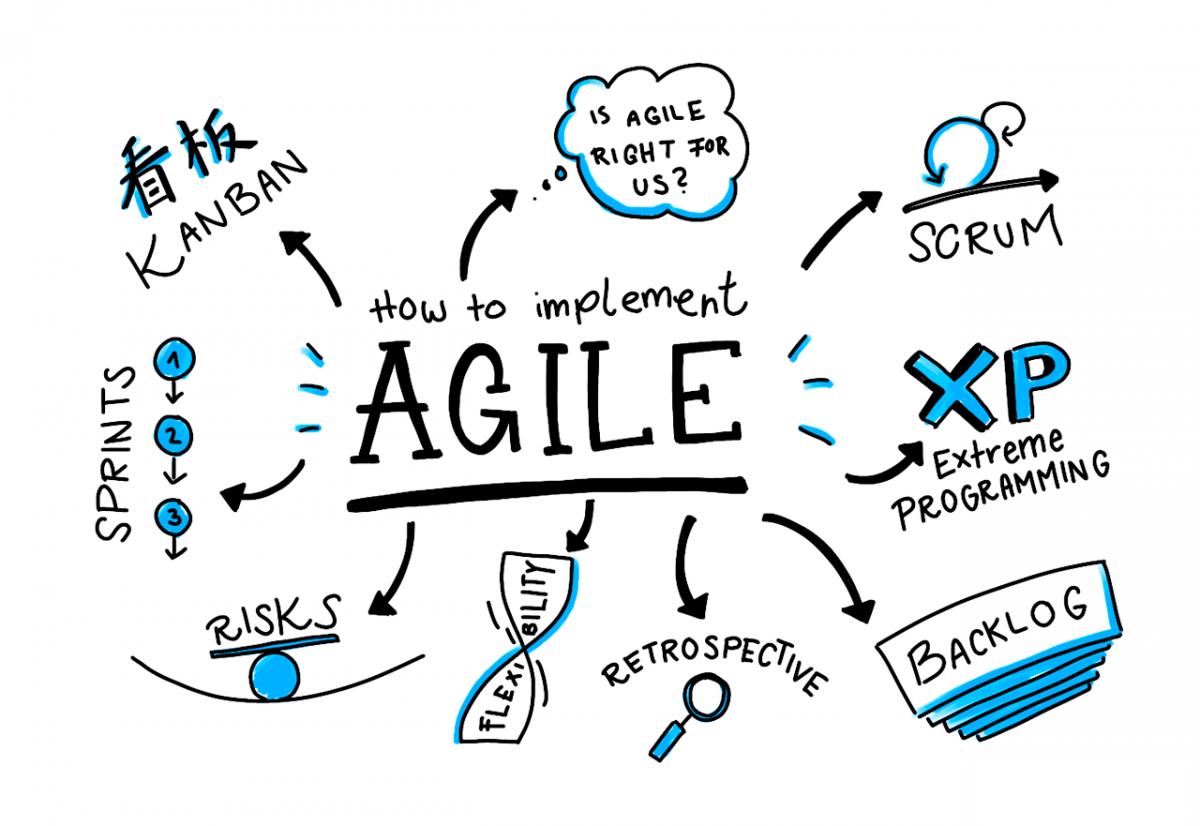
\includegraphics[width=1\columnwidth]{immagini/scrum.png}
    \caption{\label{fig:agile_scrum}Modello Agile - SCRUM}
\end{figure}
Sulla base di tali considerazioni, in accordo con l'azienda, la scelta sulla metodologia di sviluppo è ricaduta sul modello di lavoro agile\footnote{\href{Modello agile: URL: https://agilemanifesto.org/iso/it/manifesto.html}{https://agilemanifesto.org/iso/it/manifesto.html}} utilizzando il framework Scrum\footnote{Framework Scrum. URL: \href{https://it.wikipedia.org/wiki/Scrum\_(informatica)}{https://it.wikipedia.org/wiki/Scrum\_(informatica)}}. Tale framework viene adattato dell'azienda nel seguente modo:
\begin{itemize}
    \item Team di sviluppo: ogni progetto viene assegnato a più macro-team di sviluppo, composto mediamente da cinque o sei persone, come per esempio esiste il team per lo sviluppo del backend, per la realizzazione del frontend ed altro. Nel caso del progetto Consierge Croccante è stato organizzato un micro-team di due persone per il backend e una sola persona del reparto grafica per il frontend;
    
    \item Sviluppo per incremento: l’azienda Crispy Bacon adotta appieno questo approccio di sviluppo, creando di volta in volta liste di funzionalità da implementare per l'incremento successivo;
    
    \item Scrum: la riunione che rappresenta lo Scrum viene effettuata ogni tre giorni dal micro-team che si occupa del backend, in presenza del CFO e fondatore Damiano Buscemi;
    
    \item ScrumMaster: all'interno del micro-team il tutor aziendale ha ricoperto il ruolo di ScrumMaster;
    
    \item Sprint: il concetto di sprint definito nel framework Scrum viene applicato ed eseguito appieno dall'azienda. Uno sprint è stato disposto per la durata di circa due settimane;
    
\end{itemize}

\section{Tecnologie utilizzate}
\subsection{Node.js}
\label{nodejs}
Per la realizzazione del codice è stato scelto di utilizzare come linguaggio Node.js, una runtime multipiattaforma orientato agli eventi per l'esecuzione di codice JavaScript Server-side. Tale scelta è motivata dal fatto che i servizi implementati offrono API e pacchetti per questo linguaggio. Node.js consente di utilizzare JavaScript per scrivere codice da eseguire lato server, questo permette quindi di eseguire il codice sui servizi cloud computing quali Amazon Lambda. Altra particolarità di NodeJs la sua architettura orientata agli eventi che rende possibile l’inserimento di input/outputn asincrono. 

\subsection{Alexa Presentation Language}
Come accennato il progetto è costituito da un'interfaccia grafica che servirà di supporto al compimento del dialogo con la Skill. Per ottenere ciò è stato scelto di utilizzate Alexa Presentation Language\footnote{Alexa Presentation Language. URL: \href{https://developer.amazon.com/it/docs/alexa-presentation-language/apl-overview.html}{https://developer.amazon.com/it/docs/alexa-presentation-language/apl-overview.html}} messo a disposizione da Amazon. Esso permette di sviluppare il software con esperienze vocali e visive utilizzando layout. Si ha pertanto la flessibilità di sviluppare Skill multimodali con elementi visivi, tra cui grafica, immagini e la personalizzazione di output per dispositivi diversi. Quando si progetta utilizzando Alexa Presentation Language, vengono creati dei documenti APL, ovvero file JSON inviati dalla Skill al dispositivo. Quest'ultimo elabora il documento APL, importa immagini e dati per poi mostrare il risultato.

\subsection{Servizi Amazon Web Service}
\label{serivizi-aws}
AWS offre un ecosistema popolato da numerosissimi servizi già connessi tra loro. La scelta quindi di utilizzare tale ecosistema risulta la più conveniente e la più ottimale. Pertanto nel progetto vengono utilizzati i seguenti servizi:
\begin{itemize}
    \item AWS IAM: per gestire la sicurezza e gli accesso ai servizi e risorse di AWS
    \item AWS Cloud Watch: per monitorare e osservare l'esecuzione delle funzioni
    \item AWS DynamoDB: per il servizio di database non relazionale 
    \item AWS Lambda: per eseguire codice senza dover effettuare il provisioning e gestire server
    \item AWS SES: per il servizio di invio mail 
    \item AWS S3: per il servizio di storage di oggetti 
\end{itemize}

\subsection{Google Calendar}
Obbiettivo importante del prodotto è quello di poter consultare un calendario dove vengono trascritti gli impegni, eventi e appuntamenti dell'azienda. La scelta è ricaduta su l'utilizzo di Google Calendar, già utilizzado da Crispy Bacon, ovvero un sistema di calendari realizzato da Google che offre la possibilità di creare più calendari, di condividerli e importarli da altri servizi online. Difatti, quest'ultima caratteristica, agevola il collegamento tra Skill e calendario grazie a pacchetti ed API documentate.

\subsection{Slack}
Per l'invio di notifiche la scelta ricade su Slack, uno strumento software che permette di inviare messaggi in modo istantaneo, già conosciuto ed utilizzato da Crispy Bacon. Tale softfware agevola il collegamento tra Skill e la notifica istantanea grazie ad API pubbliche e documentate.  

\begin{figure}[H] 
    \centering 
    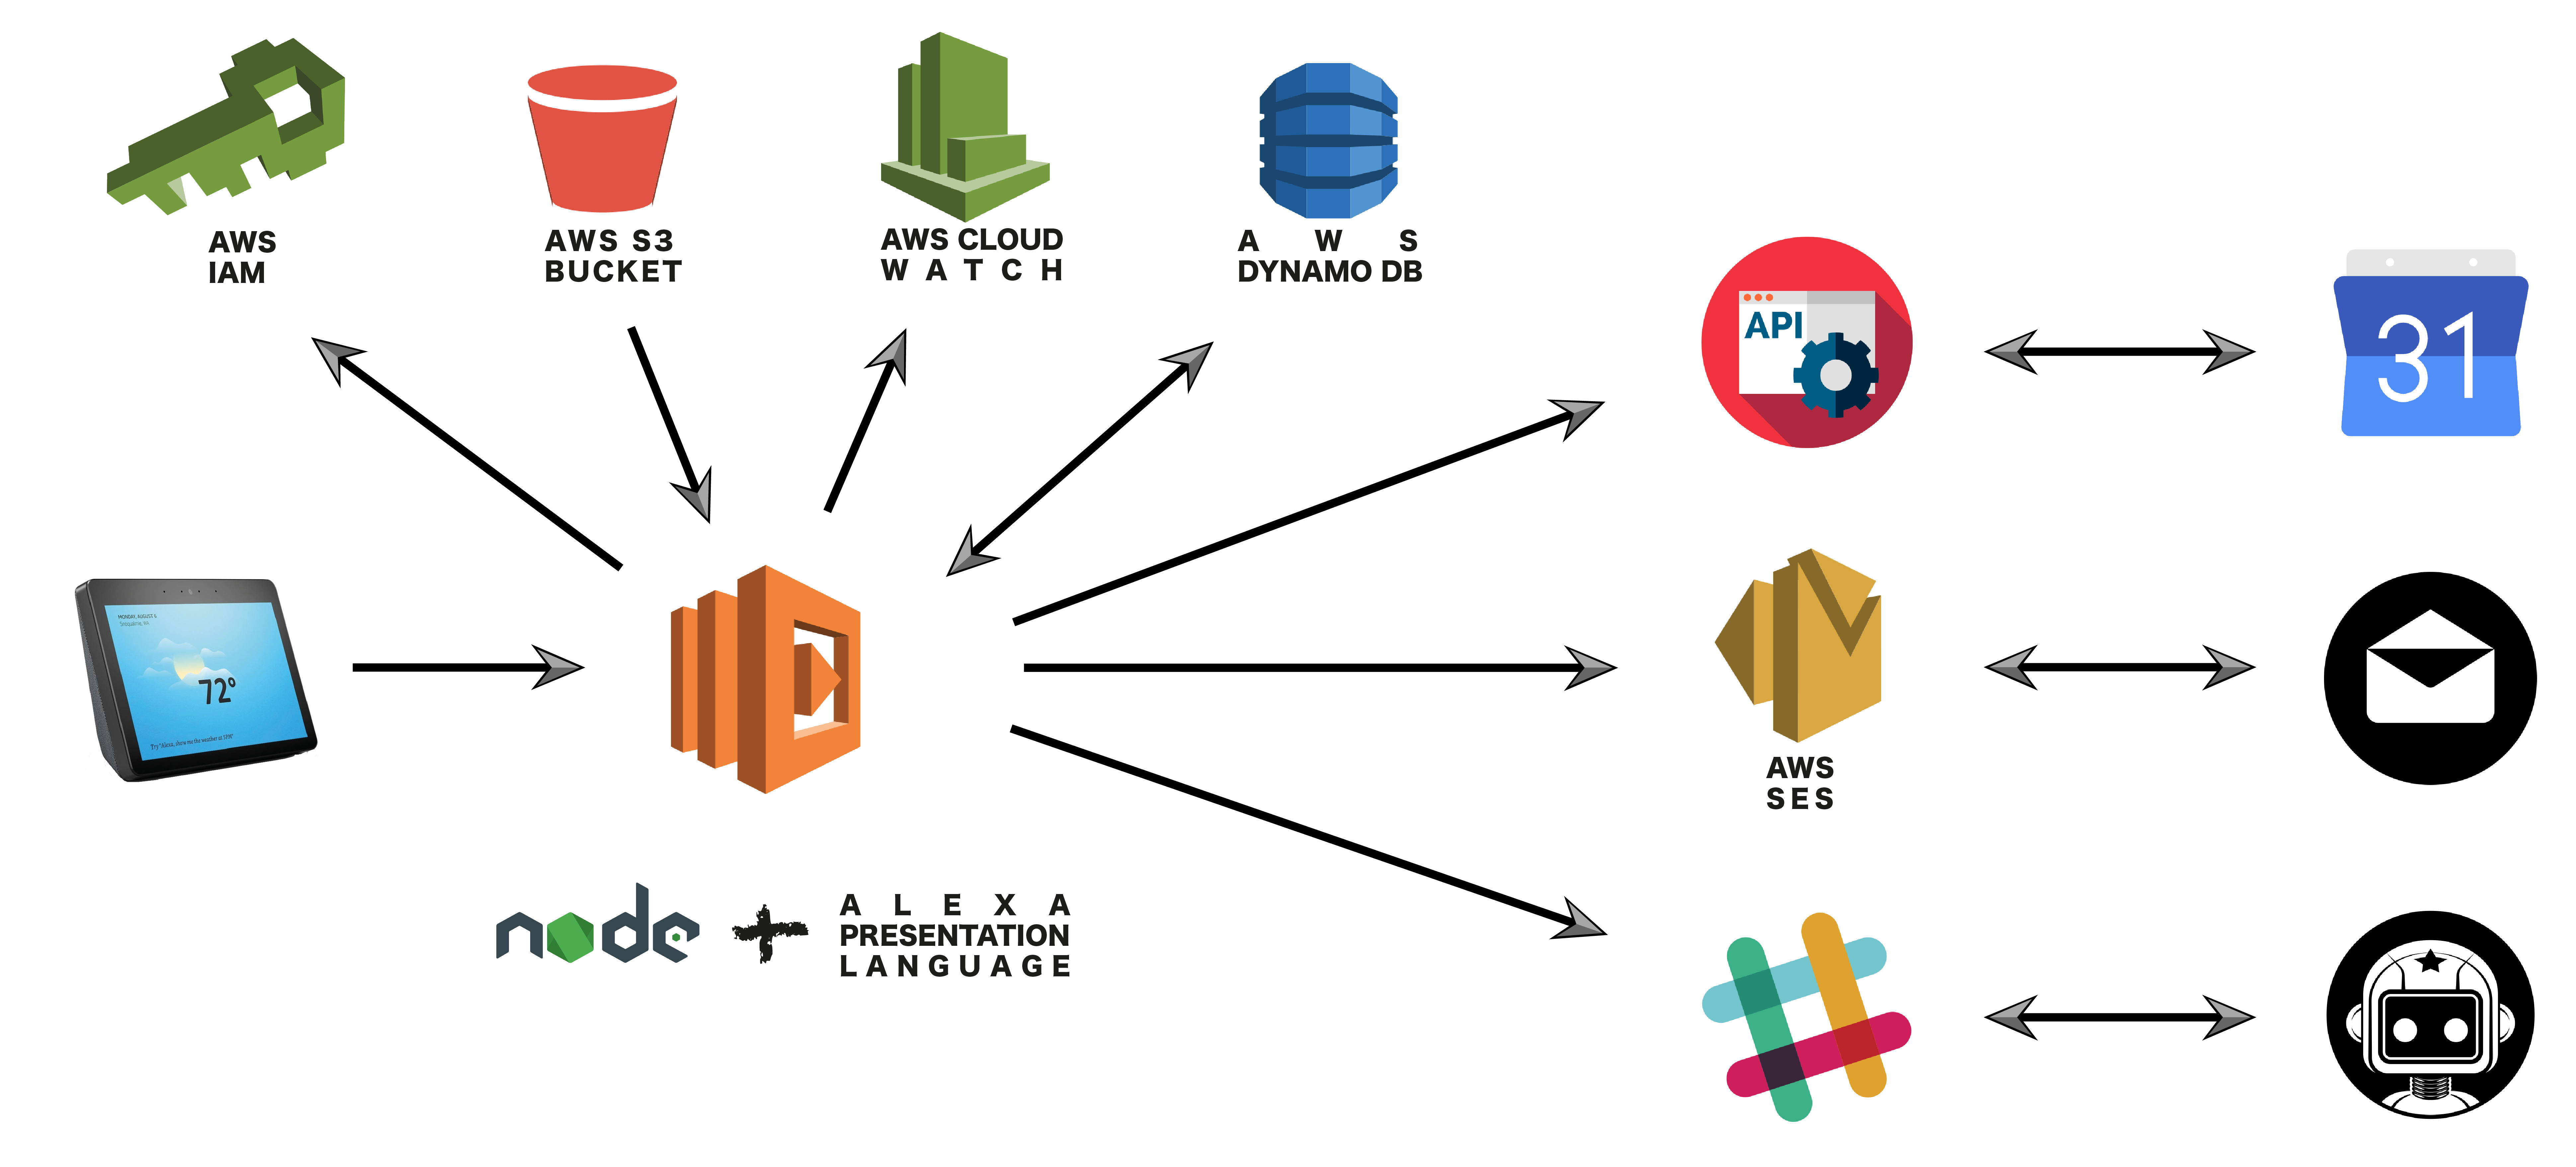
\includegraphics[width=1\columnwidth]{immagini/architettura.png}
    \caption{\label{fig:architettura}Architettura progetto C.C.}
\end{figure}

\section{Strumenti utilizzati}
\subsection{Alexa Developer Console}
Per realizzare la Skill è essenziale l'uso di Alexa Developer Console\footnote{Alexa Developer Console. URL: \href{https://developer.amazon.com/it/docs/devconsole/about-the-developer-console.html}{https://developer.amazon.com/it/docs/devconsole/about-the-developer-console.html}}, una console per gli sviluppatori che organizza lo sviluppo nelle seguenti attività principali:
\begin{itemize}
    \item Build: per realizzare e impostare la Skill creata, configurare il modello di interazione e specificare gli endpoint per il servizio.
    \item Test: per testare le Skill con l'assistente Alexa usando testo o voce.
    \item Distribuzione: per vedere in anteprima come appariranno le Skill nello store.
    \item Certificazione: per convalidare la Skill creata, eseguire test di pre-certificazione e infine inviare la Skill per la certificazione.
    \item Analytics: per rivedere le metriche relative alle Skill create.
\end{itemize}

\subsection{Amazon Echo Show}
Per vedere e testare il prodotto finale si è usato l'Amazon Echo Show, uno smart display da 10" che integra l’assistente vocale Amazon Alexa. Controllabile con la voce, è in grado di interagire con gli utenti, eseguire diversi comandi vocali oltre che mostrare i contenuti direttamente sullo schermo touch.

\subsection{NPM}
\label{npm}
Per installare i pacchetti necessari è stato utilizzato npm, il principale software per gestire i moduli di Node.js e consente di condividere il codice per problemi tipici tra gli sviluppatori JavaScript. La filosofia alla base di tale gestore è quella che se un problema è stato già risolto da altri programmatori deve esser possibile utilizzare la soluzione condivisa messa a disposizione degli altri utenti. npm oltre a consentire il riuso del codice, consente di tenerlo costantemente sotto controllo in modo da aggiornarlo. npm suddivide inoltre il codice in package, ovvero una directory che contiene uno o più file insieme, dove un file chiamato package.json contiene i dati relativi al pacchetto.

\subsection{Gitlab}
Il versionamento degli applicativi viene fatto tramite Git\footnote{Git. URL: \href{https://git-scm.com/}{https://git-scm.com/}} e i repository sono ospitati su Gitlab\footnote{Gitlab. URL: \href{https://about.gitlab.com/}{https://about.gitlab.com/}} in un server dedicato dell'azienda. GitLab è una piattaforma che permette la gestione centralizzata dei repository Git, permettendo l'amministrazione dei permessi d'accesso tramite una semplice interfaccia grafica. Tutti gli applicativi e le configurazioni dell'infrastruttura vengono ospitati sulla piattaforma e il versionamento segue regole del Git-Flow dove le funzionalità nuove vengono sviluppate su un branch dedicato, per poi essere spostate successivamente nei branch di sviluppo, accettazione e infine produzione.

\subsection{Ambiente di sviluppo}
L’azienda non ha posto alcuna limitazione per quanto riguarda gli IDE lasciando libero arbitrio sulla scielta. Necessitando il progetto di diversi linguaggi quali Node.js e JSON la scelta è ricaduta su Visual Studio Code\footnote{Visual Studio Code. URL: \href{https://code.visualstudio.com/}{https://code.visualstudio.com/}}, IDE sviluppato da Microsoft\footnote{Microsoft. URL: \href{https://www.microsoft.com/}{https://www.microsoft.com/}} e consigliato per lavorare con progetti multi linguaggio, in quanto estensibile tramite plugin per supportare la maggior parte dei linguaggi di programmazione.
%**************************************************************
\section{Organizzazione del testo}
Il documento presenta la seguente struttura:
\begin{itemize}
    \item Capitolo 1: Introduzione comprende la descrizione generale dell'azienda ospitante e del relativo metodo di lavoro, una contestualizzazione ed illustrazione del progetto di stage ed infine la presentazione della struttura del documento
    \item Capitolo 2: Analisi dei Requisiti si tratta di una descrizione dettagliata della fase di analisi dei requisiti portata a termine dal candidato
    \item Capitolo ??
    \item Capitolo ??
    \item Capitolo ??
\end{itemize}




             
% !TEX encoding = UTF-8
% !TEX TS-program = pdflatex
% !TEX root = ../tesi.tex

%**************************************************************
\chapter{Analisi dei Requisiti}
\label{cap:processi-metodologie}
%**************************************************************
Durante il primo periodo di tirocinio è stata svolta la fase di Analisi dei Requisiti, necessaria alla comprensione del dominio e al soddisfacimento della richiesta. Inizialmente è stato effettuato un incontro con il tutor aziendale con il quale sono stati rilevati i requisti obbligatori richiesti dall'azienda da cui è stato possibile identificare un insieme di funzionalità necessarie alla Skill. Successivamente è stato realizzato il documento contenente tutti gli studi di analisi che hanno favorito una buona e corretta progettazione del prodotto. Dalla raccolta dei dati e dalle analisi fatte è stata elaborata una visione ad alto livello del sistema e dei rispettivi casi d’uso. Sono stati inoltre identificati quei punti critici in grado di determinare, in larga misura, la forma finale del prodotto.
La fase di analisi si è infine conclusa con lo studio della VUI (Voice User Interface), e della GUI (Graphical User Interface), che caratterizzano l'esperienza d'uso del prodotto finale. 

%**************************************************************
\section{Obbiettivo}
L’obiettivo del progetto di stage è la realizzazione di una Skill per l’assistente vocale Alexa che sia in grado di accogliere clienti, postini e corrieri all'ingresso degli uffici e notificare in maniera automatica la persona interessata nell'arrivo del visitatore. La Skill è concepita per essere installata sui dispositivi in commercio da Amazon, in particolare sul dispositivo Echo Show 2018. L’obiettivo è quindi quello di realizzare un concierge virtuale che accolga il visitatore e riceva da esso informazioni per mezzo di una conversazione e l’uso di messaggi attraverso lo schermo touch integrato nel dispositivo. In fine tali dati elaborati dai processi di controllo per inviare notifiche al personale.

\subsection{Cliente finale}
Il cliente finale a cui è destinato il prodotto è l’azienda Crispy Bacon Srl, la quale necessita, per ovvi motivi, di un sistema automatizzato che svolga il ruolo di Concierge all'entrata degli uffici. L’azienda desidera, con questo prodotto, realizzare uno prototipo da poter rendere spendibile tale servizio proponendolo come pacchetto preconfezionato o da personalizzare al fine di venderlo a clienti terzi.

\section{Attori coinvolti}
Dall'analisi fatta sono emersi i seguenti attori, intesi come persone coinvolte nell'utilizzo della Skill:
\begin{itemize}
    \item Visitatore
        \begin{itemize}
            \item Persona avente appuntamento
            \item Persona non avente appuntamento
            \item Postino
            \item Corriere
        \end{itemize}
    \item Personale di Crispy Bacon
\end{itemize}

\section{Requisiti richiesti}
I requisiti emersi e richiesti dall'azienda sono stati elaborati e analizzati. Tali requisiti sono interpretabili in tre diversi modi, tutti sotto il presupposto che questi siano in qualche modo una necessità.
\begin{itemize}
    \item Requisito utente: dal punto di vista dell'utente, è una capacità necessaria per risolvere un problema o raggiungere un obbiettivo.
    \item Requisito software: dal punto di vista della soluzione, è una capacità che deve essere posseduta dal sistema per adempiere all'obiettivo.
    \item Dal punto di vista della documentazione, come una descrizione documentata di una capacità interpretata come un requisito utente o software.
\end{itemize}
\subsubsection{Identificazione dei Requisiti}
Per identificare i requisti viene utilizzata la seguente notazione tabellare con un codice che lo identifica e la corrispettiva descrizione affianco.
\begin{center}
    R.x.y
\end{center}
\begin{itemize}
    \item R: identifica il requisito
    \item x: identifica l'importanza di tale requisito che può essere
        \begin{itemize}
            \item O obbligatorio
            \item D desiderabile
        \end{itemize}
    \item y: identifica un valore numerico progressivo a partire da 1
\end{itemize}
In merito allo studio di analisi fatto all'inizio del periodo di tirocinio sono emersi i seguenti requisti, \textbf{considerati obbligatori} per il soddisfacimento del risultato atteso dal prodotto finale.
\begin{center}
	\centering
	\renewcommand{\arraystretch}{1.5}
	\rowcolors{3}{tableLight}{}
	\begin{longtable}{  p{2.5cm} p{9.8cm} }
		\rowcolor{tableHead}
		\textbf{\textcolor{white}{Identificativo}} & \textbf{\textcolor{white}{Requisito}} \\
		\endhead  
		RO1 & La Skill al momento dal lancio deve presentare un messaggio di benvenuto (VUI) \\
		RO2 & La Skill al momento dal lancio deve presentare un messaggio di benvenuto (GUI) \\
		RO3 & La Skill al momento dal lancio deve presentare un elenco essenziale e sintetico delle azioni da fare (VUI) \\ 
		RO4 & La Skill al momento dal lancio deve presentare un elenco essenziale e sintetico delle azioni da fare  (GUI) \\
		RO5 & La Skill deve poter ricevere le informazioni necessarie dal visitatore per mezzo di una conversazione impostata (VUI)  \\
		RO6 & La Skill deve poter riportare le informazioni ottenute dal visitatore e riportarle nello schermo del dispositivo (GUI) \\
		RO7\label{RO7} & La Skill deve poter utilizzare e interrogare il servizio di calendarizzazione con le informazioni ottenute dal visitatore al fine di notificare l'interessato della visita.\\
		RO8\label{RO8} & La Skill deve notificare o inviare una notifica all'interessato della visita.\\
		RO9 & La Skill deve riportare sullo schermo del dispositivo delle funzioni disponibili in base alle risposte ricevute dal dialogo fatto con il visitatore (GUI - VUI)\\
		\rowcolor{white}
		\caption{Tabella tracciamento requisiti obbligatori}
	\end{longtable}
\end{center}
Infine nell'analisi sono stati individuati anche i \textbf{requisiti desiderabili}, considerati non strettamente necessari ma di valore aggiunto al prodotto atteso.
\begin{center}
	\centering
	\renewcommand{\arraystretch}{1.5}
	\rowcolors{3}{tableLight}{}
	\begin{longtable}{  p{2.5cm} p{9.8cm} }
		\rowcolor{tableHead}
		\textbf{\textcolor{white}{Identificativo}} & \textbf{\textcolor{white}{Requisito}} \\
		\endhead  
		RD1 & La Skill una volta verificata la presenza del visitatore informa quest'ultimo se l'interessato risulta non reperibile se assente \\
		RD2 & La Skill deve poter registrare il momento in cui il visitatore inizia l'incontro con la persona cercata nel caso di un appuntamento \\
		RD3 & La Skill deve poter registrare il momento in cui il visitatore termina l'incontro con la persona cercata nel caso di un appuntamento \\
		\rowcolor{white}
		\caption{Tabella tracciamento requisiti desiderabili}
	\end{longtable}
\end{center}
\section{Casi d'uso}
Dalle analisi fatte e dai dati raccolti sono stati studiati i requisiti funzionali, ovvero i casi d'uso del prodotto Concierge Crocante, che permettono di descrivere interazioni tra gli utenti, tra il sistema e come quest'ultimo deve essere utilizzato. Durante lo stage sono stati così esaminate le sequenze di passi che descrivono interazioni e la rappresentazione di possibilità, che hanno in comune uno scopo finale per un utente (attore).\\[0.4cm]
Gli attori emersi nell'analisi dei casi d’uso svolgono il ruolo dell'utente nell'interazione con la Skill per raggiungere l’obiettivo prefissato. In questa analisi sono stati individuati gli attori:
    \begin{itemize}
        \item Utente generico, che può essere generalizzato in:
            \begin{itemize}
                \item Visitatore
                    \begin{itemize}
                        \item avente appuntamento
                        \item non avente appuntamento
                        \item postino
                        \item corriere
                    \end{itemize}
                \item Persona cercata
        \end{itemize}
    \end{itemize}
Di seguito viene riportato lo schema degli attori individuati utilizzando lo standard UML 2.0
\begin{figure}[H] 
    \centering 
    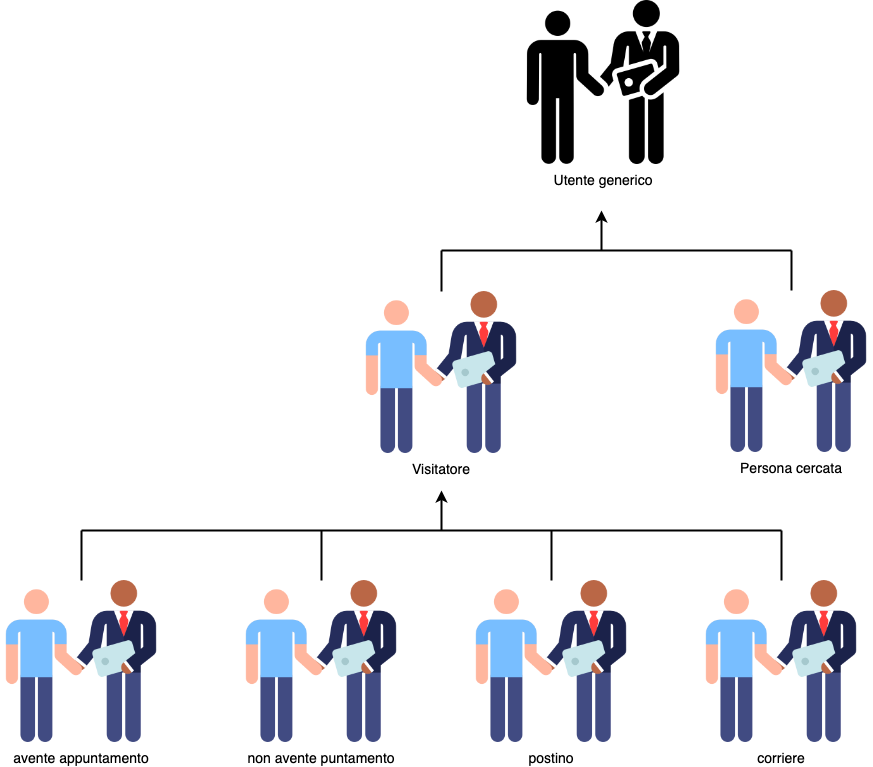
\includegraphics[width=0.9\columnwidth]{immagini/attori.png}
    \caption{\label{fig:attori}Utenti del sistema}
\end{figure}
\subsection{Casi d'uso - Visitatore}
Durante il periodo di tirocinio, la fase di analisi dei casi d'uso è da considerarsi divisa in due parti simili fra loro: quella dedicata al visitatore, ovvero colui che si presenta negli uffici dell'azienda avente un appuntamento registrato in calendario, o che semplicemente si presenta senza preavviso, e il servizio di consegna pacchi svolto dal postino o dal corriere. In entrambe le parti gli attori avvieranno la Skill installata nel dispositivo Amazon Echo Show e seguiranno le istruzioni riportate a voce dall'assistente vocale oppure mostrate a video dal display. In questa sezione viene riporta una rappresentazione grafica dei casi d'uso dell'utente identificato come "Visitatore avente appuntamento", che descrive le interazioni che l'attore svolge con il sistema.  
\begin{figure}[H] 
    \centering 
    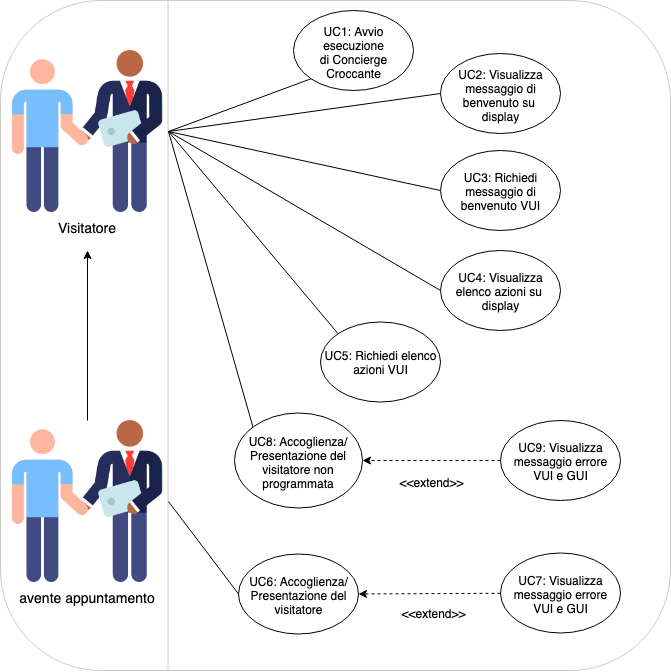
\includegraphics[width=1\columnwidth]{immagini/casi_duso1.png}
    \caption{\label{fig:casi_duso_visitatore}Casi d'uso visitatore avente appuntamento}
\end{figure}
Dall'elaborazione di tale analisi sono quindi emersi i seguenti casi d'uso riportati:
\begin{center}
	\centering
	\renewcommand{\arraystretch}{1.5}
	\rowcolors{3}{tableLight}{}
	\begin{longtable}{  p{2.5cm} p{9.8cm} }
		\rowcolor{tableHead}
		\textbf{\textcolor{white}{Identificativo}} & \textbf{\textcolor{white}{Descrizione}} \\
		\endhead  
		
		UC1 &  \textit{Attori}: persona con o senza appuntamento \newline \textit{Scopo}: l'utente può avviare Concierge Croccante \newline \textit{Pre-condizione}: il dispositivo Amazon deve aver avviato \mbox{l'assistente} Alexa \newline \textit{Post-condizione}: l'utente ha avviato Concierge Croccante \\
		
		UC2 &  \textit{Attori}: persona \newline \textit{Scopo}: l'utente riceve un messaggio di benvenuto sul display del dispositivo \newline \textit{Pre-condizione}: la Skill Concierge Croccante deve essere stata avviata \newline \textit{Post-condizione}: l'utente riceve un messaggio di benvenuto sul display del dispositivo \\
		
		UC3 &  \textit{Attori}: persona \newline \textit{Scopo}: l'utente riceve un messaggio vocale di benvenuto dalla Skill \mbox{Concierge} Croccante \newline \textit{Pre-condizione}: la Skill Concierge Croccante deve essere stata avviata \newline \textit{Post-condizione}: l'utente riceve un messaggio vocale dalla Skill Concierge Croccante\\
		
		UC4 &  \textit{Attori}: persona \newline \textit{Scopo}: l'utente visualizza l'elenco sintetico ed essenziale di azioni sul \mbox{display} del dispositivo \newline \textit{Pre-condizione}: la Skill Concierge Croccante deve essere stata avviata \newline \textit{Post-condizione}: l'utente visualizza l'elenco di azioni sul display del dispositivo \\
		
		UC5 &  \textit{Attori}: persona \newline \textit{Scopo}: viene esposto all'utente l'elenco sintetico ed essenziale di azioni \newline \textit{Pre-condizione}: la Skill Concierge Croccante deve essere stata avviata \newline \textit{Post-condizione}: viene esposto all'utente l'elenco di azioni disponibili da Concierge Croccante \\
		
		UC6 &  \textit{Attori}: persona con appuntamento \newline \textit{Scopo}: l'utente può annunciarsi per essere accolto dalla persona cercata \newline \textit{Pre-condizione}: la Skill Concierge Croccante deve essere stata avviata \newline \textit{Post-condizione}: l'utente si annuncia \\
		
		UC7 &  \textit{Attori}: persona con appuntamento \newline \textit{Scopo}: viene visualizzato un messaggio, su display e vocale, di errore specifico per l'eccezione riscontrata \newline \textit{Pre-condizione}: la Skill Concierge Croccante deve essere stata avviata \newline \textit{Post-condizione}: l'utente riceve un messaggio su display e vocale di errore\\
		
		UC8 &  \textit{Attori}: persona \newline \textit{Scopo}: l'utente può annunciarsi per essere accolto dalla persona cercata \newline \textit{Pre-condizione}: la Skill Concierge Croccante deve essere stata avviata \newline \textit{Post-condizione}: l'utente si annuncia \\
		
		UC9 &  \textit{Attori}: persona \newline \textit{Scopo}: viene visualizzato un messaggio, su display e vocale, di errore specifico per l'eccezione riscontrata \newline \textit{Pre-condizione}: la Skill Concierge Croccante deve essere stata avviata \newline \textit{Post-condizione}: l'utente riceve un messaggio su display e vocale di errore\\
		
		\rowcolor{white}
		\caption{\label{tab:UC_persona}Tabella casi d'uso persona con appuntamento e non}
	\end{longtable}
\end{center}
\begin{figure}[H] 
    \centering 
    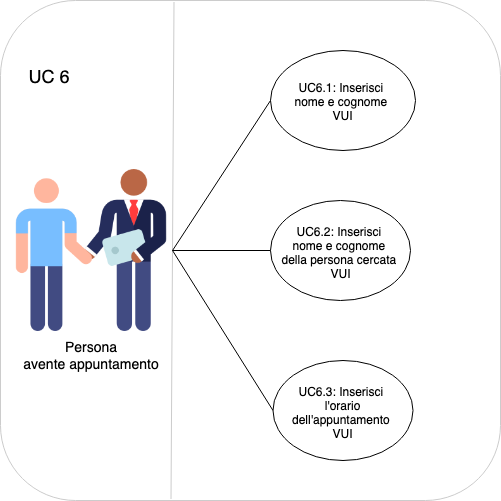
\includegraphics[width=0.7\columnwidth]{immagini/casi_duso2.png}
    \caption{\label{fig:sotto_casi_duso_visitatori1}Sotto casi d'uso visitatore avente appuntamento}
\end{figure}
\begin{center}
	\centering
	\renewcommand{\arraystretch}{1.5}
	\rowcolors{3}{tableLight}{}
	\begin{longtable}{  p{2.5cm} p{9.6cm} }
		\rowcolor{tableHead}
		\textbf{\textcolor{white}{Identificativo}} & \textbf{\textcolor{white}{Descrizione}} \\
		\endhead  
		
		UC6.1 &  \textit{Attori}: persona con o senza appuntamento \newline \textit{Scopo}: l'utente inserisce/dice il suo nome e cognome \newline \textit{Pre-condizione}: la Skill Concierge Croccante deve essere stata avviata \newline \textit{Post-condizione}: l'utente ha inserito/detto il suo nome e cognome \\
		
		UC6.2 &  \textit{Attori}: persona con o senza appuntamento \newline \textit{Scopo}: l'utente inserisce/dice il nome e cognome della persona che cerca \newline \textit{Pre-condizione}: la Skill Concierge Croccante deve essere stata avviata \newline \textit{Post-condizione}: l'utente ha inserito/detto il suo nome e cognome della persona cercata \\
		
		UC6.3 &  \textit{Attori}: persona con o senza appuntamento \newline \textit{Scopo}: l'utente inserisce/dice l'orario di appuntamento \newline \textit{Pre-condizione}: la Skill Concierge Croccante deve essere stata avviata \newline \textit{Post-condizione}: l'utente ha inserito/detto l'orario di appuntamento \\
		
		\rowcolor{white}
		\caption{Tabella sotto casi d'uso persona con appuntamento e non}
	\end{longtable}
\end{center}
\begin{figure}[H] 
    \centering 
    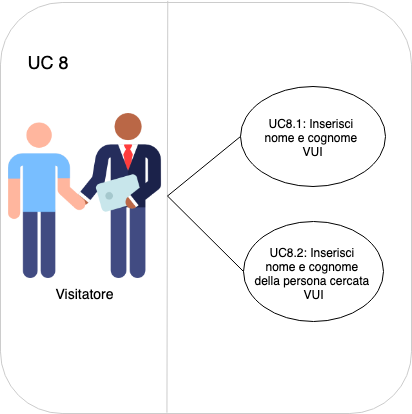
\includegraphics[width=0.7\columnwidth]{immagini/casi_duso21.png}
    \caption{\label{fig:sotto_casi_duso_visitatore2}Sotto casi d'uso visitatore avente appuntamento}
\end{figure}
\begin{center}
	\centering
	\renewcommand{\arraystretch}{1.5}
	\rowcolors{3}{tableLight}{}
	\begin{longtable}{  p{2.5cm} p{9.8cm} }
		\rowcolor{tableHead}
		\textbf{\textcolor{white}{Identificativo}} & \textbf{\textcolor{white}{Descrizione}} \\
		\endhead  
		
		UC8.1 &  \textit{Attori}: persona \newline \textit{Scopo}: l'utente inserisce/dice il suo nome e cognome \newline \textit{Pre-condizione}: la Skill Concierge Croccante deve essere stata avviata \newline \textit{Post-condizione}: l'utente ha inserito/detto il suo nome e cognome \\
		
		UC8.2 &  \textit{Attori}: persona  \newline \textit{Scopo}: l'utente inserisce/dice il nome e cognome della persona che cerca \newline \textit{Pre-condizione}: la Skill Concierge Croccante deve essere stata avviata \newline \textit{Post-condizione}: l'utente ha inserito/detto il suo nome e cognome della persona cercata \\

		\rowcolor{white}
		\caption{Tabella sotto casi d'uso persona con appuntamento e non}
	\end{longtable}
\end{center}
\subsection{Casi d'uso - Postino/Corriere}
La seconda parte di analisi dei casi d'uso, è dedicata al servizio di consegna dei pacchi che viene svolto dal postino o dal corriere. In questa sezione si rappresenta graficamente i casi d'uso dell'utente identificato come "Corriere", che descrive le interazioni che l'attore svolge con il sistema.
\begin{figure}[H] 
    \centering 
    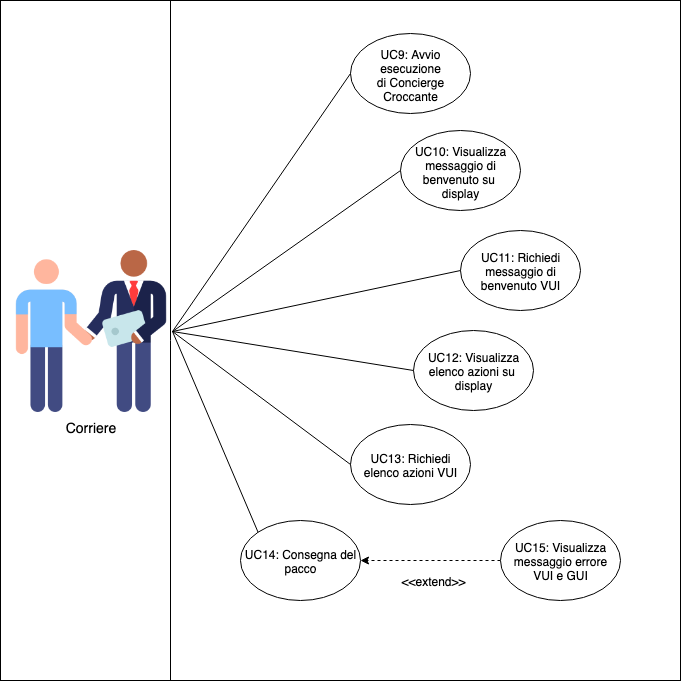
\includegraphics[width=1\columnwidth]{immagini/casi_duso3.png}
    \caption{\label{fig:casi_duso_corriere}Casi d'uso corriere}
\end{figure}
Dall'elaborazione di tale analisi sono quindi emersi i seguenti casi d'uso riportati:
\begin{center}
	\centering
	\renewcommand{\arraystretch}{1.5}
	\rowcolors{3}{tableLight}{}
	\begin{longtable}{  p{2.5cm} p{9.8cm} }
		\rowcolor{tableHead}
		\textbf{\textcolor{white}{Identificativo}} & \textbf{\textcolor{white}{Descrizione}} \\
		\endhead  
		
		
		UC9 &  \textit{Attori}: corriere \newline \textit{Scopo}: l'utente può avviare Concierge Croccante \newline \textit{Pre-condizione}: il dispositivo Amazon deve aver avviato l'assistente Alexa \newline \textit{Post-condizione}: l'utente ha avviato Concierge Croccante \\
		
		UC10 &  \textit{Attori}: corriere \newline \textit{Scopo}: l'utente riceve un messaggio di benvenuto sul display del dispositivo \newline \textit{Pre-condizione}: la Skill Concierge Croccante deve essere stata avviata \newline \textit{Post-condizione}: l'utente riceve un messaggio di benvenuto sul display del dispositivo \\
		
		UC11 &  \textit{Attori}: corriere \newline \textit{Scopo}: l'utente riceve un messaggio vocale di benvenuto dalla Skill \mbox{Concierge} Croccante \newline \textit{Pre-condizione}: la Skill Concierge Croccante deve essere stata avviata \newline \textit{Post-condizione}: l'utente riceve un messaggio vocale dalla Skill C.C.\\
		
		UC12 &  \textit{Attori}: corriere \newline \textit{Scopo}: l'utente visualizza l'elenco sintetico ed essenziale di azioni sul \mbox{display} del dispositivo \newline \textit{Pre-condizione}: la Skill Concierge Croccante deve essere stata avviata \newline \textit{Post-condizione}: l'utente visualizza l'elenco di azioni sul display del dispositivo \\
		
		UC13 &  \textit{Attori}: corriere \newline \textit{Scopo}: viene esposto all'utente l'elenco sintetico ed essenziale di azioni \newline \textit{Pre-condizione}: la Skill Concierge Croccante deve essere stata avviata \newline \textit{Post-condizione}: viene esposto all'utente l'elenco di azioni disponibili da C.C. \\
		
		UC14 &  \textit{Attori}: corriere \newline \textit{Scopo}: l'utente può consegnare un pacco \newline \textit{Pre-condizione}: la Skill Concierge Croccante deve essere stata avviata \newline \textit{Post-condizione}: l'utente consegna il pacco \\
		
		UC15 &  \textit{Attori}: corriere \newline \textit{Scopo}: viene visualizzato un messaggio, su display e vocale, di errore specifico per l'eccezione riscontrata \newline \textit{Pre-condizione}: la Skill Concierge Croccante deve essere stata avviata \newline \textit{Post-condizione}: l'utente riceve un messaggio su display e vocale di errore\\
		
		UC17 &  \textit{Attori}: corriere \newline \textit{Scopo}: l'utente per consegnare il pacco richiede la presenza di una persona specifica per una firma \newline \textit{Pre-condizione}: la Skill Concierge Croccante deve essere stata avviata \newline \textit{Post-condizione}: l'utente riceve la firma desiderata e consegna il pacco\\
		
		UC18 &  \textit{Attori}: corriere \newline \textit{Scopo}: l'utente per consegnare il pacco richiede la presenza di una persona per una firma \newline \textit{Pre-condizione}: la Skill Concierge Croccante deve essere stata avviata \newline \textit{Post-condizione}: l'utente riceve la firma desiderata e consegna il pacco\\
		\rowcolor{white}
		\caption{Tabella casi d'uso corriere}
	\end{longtable}
\end{center}
\section{Voice User Interface - VUI}
Altro aspetto importante dell'analisi è stata sulla Voice User Interface, che nel documento verrà abbreviato con l'acronimo VUI. La VUI per la Skill è l’interfaccia che rende possibile l’interazione umana parlata con il computer, utilizzando il riconoscimento vocale per comprendere comandi e domande vocali, ed infine il text to speech per riprodurre una risposta. Nel caso del progetto la VUI è rappresentata dall'assistente vocale Amazon Alexa, la quale eseguirà la Skill prodotta. Vista la ovvia complessità che presenta un'interazione umana vocale con un computer, la VUI fornita dall'assistente vocale Alexa presenta alcuni limiti che verranno analizzati successivamente in un nuovo punto del capitolo.\\
L’obbiettivo che si prefigge nel realizzare la Skill è quello di poter sostenere una conversazione, il più naturale possibile, con la persona accolta all'entrata dell'azienda Crispy Bacon. L’idea è quindi che l’ospite possa dialogare con Concierge Croccante, motivare la presenza in azienda e notificare l’interessato della visita. Dall'analisi emerge una conversazione come l'esempio seguente in formato testo di quello che si vuole ottenere dal prodotto finale:
\begin{figure}[H] 
    \centering 
    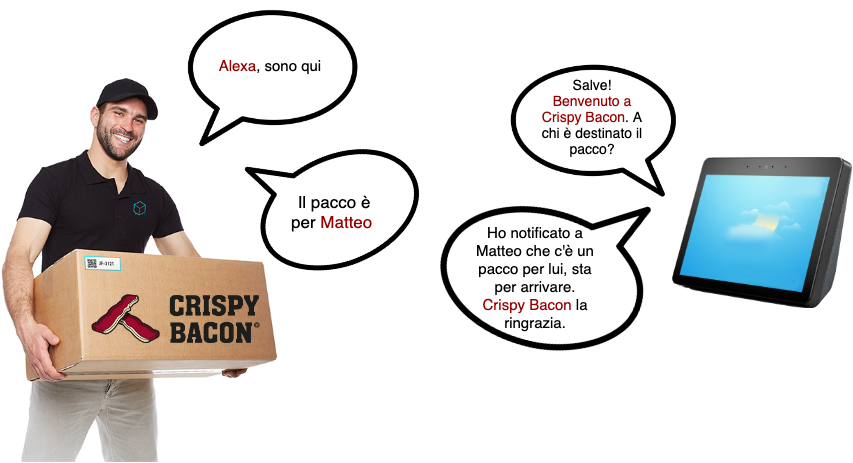
\includegraphics[width=1\columnwidth]{immagini/esempioVUI.png}
    \caption{\label{fig:esempioVUI}Esempio di conversazione}
\end{figure}
\begin{itemize}
	\item \textbf{Utente}: \textit{"Alexa, sono qui."}
	\item \textbf{Concierge}: \textit{ "Buongiorno! Benvenuto a Crispy Bacon, quale è il motivo della sua visita?"}
	\item \textbf{Utente}: \textit{"Devo consegnare un pacco."}
	\item \textbf{Concierge}: \textit{ "Chi è il destinatario del pacco?"}
	\item \textbf{Utente}: \textit{"Matteo P."}
	\item \textbf{Concierge}: \textit{ "Ho notificato a Matteo che c'è un pacco per lui, sta per arrivare."}
	\item \textbf{Concierge}: \textit{ "Crispy Bacon la ringrazia"}
\end{itemize}
La Skill Concierge Croccante necessita quindi di ricevere dati in input per poter completare il processo di accoglienza della persona entrata in azienda. È quindi necessario suddividere i dati richiesti in base alla tipo di utente:
\begin{center}
	\centering
	\renewcommand{\arraystretch}{1.5}
	\rowcolors{3}{tableLight}{}
	\begin{longtable}{  p{4.5cm} p{8.3cm} }
		\rowcolor{tableHead}
		\textbf{\textcolor{white}{Tipo di utente}} & \textbf{\textcolor{white}{Dati da raccogliere}} \\
		\endhead  
		
		Persona senza \mbox{appuntamento} &  - Proprio nome \newline - Proprio cognome \newline - Nome persona cercata  \newline - Cognome persona cercata \\
		Persona con \mbox{appuntamento} &  - Proprio nome \newline - Proprio cognome \newline - Nome persona cercata  \newline - Cognome persona cercata \newline - Orario dell'appuntamento \\
		Corriere &  - Il proprio titolo (corriere) \newline - Nome della persona interessata \newline - Cognome della persona interessata \\
		Postino &  - Il proprio titolo (postino) \newline - Nome della persona interessata \newline - Cognome della persona interessata \\
		\rowcolor{white}
		\caption{Tabella tipologia dati per tipo di utente}
	\end{longtable}
\end{center}
\subsection{Voice Flow}
\section{Graphical User Interface - GUI}
             
%% !TEX encoding = UTF-8
% !TEX TS-program = pdflatex
% !TEX root = ../tesi.tex

%**************************************************************
\chapter{Progettazione e codifica}
\label{cap:progettazione}
In questo capitolo verrà tratta il secondo periodo del tirocinio: la progettazione e la codifica. Questa parte, avvenuta dopo l'Analisi dei Requisiti, è da ritenersi importante per progetto in quanto ha occupato gran parte del tempo lavorativo. Il primo passo è stato eseguire la progettata dell'architettura, in modo che i servizi necessari fossero correttamente configurati prima del loro effettivo utilizzo. Successivamente è stata eseguita la stesura del codice per la realizzazione della Skill. Nei paragrafi successivi seguiranno porzioni di codice significativo per la loro importanza e per il funzionamento di determinate funzionalità e/o servizi. Importante ricordare che il codice implementato e mostrato sarà in Node.js come quanto detto nel nel paragrafo \hyperref[nodejs]{1.4.1}. 
%**************************************************************
\section{Architettura}
Come riportato nel paragrafo \hyperref[serivizi-aws]{1.4.3}, il progetto si basa interamente sui servizi offerti dall'ecosistema Amazon. Di conseguenza è risultato facile ed immediato impostare i servizi dell'architettura in modo da rendere il tutto efficacie ed efficiente. In questo paragrafo si andrà a comprendere cosa offre ogni singolo servizio di AWS e come esso è stato impostato per il suo corretto funzionamento nella Skill.

\section{Configurazione servizi Amazon Web Service}
\subsection{AWS SES}
Amazon SES\footnote{AWS SES. URL: \href{https://aws.amazon.com/it/ses/}{https://aws.amazon.com/it/ses/}} (Simple Email Service) è un servizio di invio e-mail basato sul cloud messo a disposizione da Amazon per gli sviluppatori di applicazioni. Tale servizio è da considerarsi vantaggioso in quanto è affidabile e a costo ridotto, utile per qualunque tipo di azienda ed ideale per la realizzazione del progetto.
\newpage
\noindent Per utilizzare AWS SES è necessario impostare il servizio visitando la pagina\footnote{AWS SES. URL: \href{https://aws.amazon.com/it/ses/}{https://aws.amazon.com/it/ses/}} dedicata ed eseguire le istruzioni riportate:
\\[0.5cm]
\begin{minipage}{0.5\textwidth}
	\begin{figure}[H]
		
\includegraphics[width=6cm]{immagini/ses.png}
		\caption{\label{fig:icona_aws_ses}Icona AWS SES}
	\end{figure}
\end{minipage}
\begin{minipage}{0.5\textwidth}
	\begin{itemize}
		\item Eseguire l'accesso con le proprie credenziali di account AWS;
    	\item Una volta fatto l'accesso cliccare \texttt{Email Addresses} sul pannello a sinistra;
    	\item Cliccare \texttt{Verify a New Email Address};
    	\item Inserire l'indirizzo e-mail da verificare il quale verrà utilizzato per inviare le notifiche;
    	\item Confermare la verifica cliccando sul URL contenuto nella e-mail ricevuta.
	\end{itemize}
\end{minipage}
\\[0.5cm]
Il procedimento descritto sopra non fa altro che verificare l'indirizzo e-mail con il quale si andrà ad inviare messaggi di posta elettronica tramite la Skill. Amazon infatti permette l'uso di questo servizio solo se il mittente e il destinatario delle e-mail sono indirizzi verificati. Per completare la configurazione è necessario di verificare il dominio delle caselle mail di Crispy Bacon: 
\begin{itemize}
    \item Sempre all'interno di AWS SES cliccare su \texttt{Domains} sul pannello a sinistra;
    \item Cliccare in altro \texttt{Verify a New Domains};
    \item Inserire il dominio degli indirizzi e-mail destinatari delle mail, nel caso del progetto \textit{crispybacon.store};
    \item Infine cliccare su \texttt{Verify This Domain} per terminare il processo di verifica.
\end{itemize}
A questo punto è possibile mandare messaggi e notifiche tramite mail utilizzando l'indirizzo verificato prima.
\newpage
\subsection{AWS S3}
Amazon S3\footnote{AWS S3. URL: \href{https://aws.amazon.com/it/s3/}{https://aws.amazon.com/it/s3/}} (S3 = Simple Storage Service) è un servizio di storage di oggetti che offre scalabilità, disponibilità dati, sicurezza e prestazioni all'avanguardia. Queste caratteristiche offre alle industrie di qualsiasi dimensione la possibilità di archiviare e proteggere una qualsiasi quantità di dati per qualunque genere di uso: come ad esempio per siti Web, applicazioni mobile, backup e ripristino, archiviazione, applicazioni enterprise\footnote{Iintegrazione tra diversi tipi di sistemi informatici con l'utilizzo di software e soluzioni architetturali}, dispositivi IoT\footnote{Internet of Things: neologismo utilizzato per dare un nome agli oggetti reali connessi ad internet} e analisi di big data. Amazon S3 offre una gestione semplice di utilizzo grazie alla sua pagina web dedicata, all'interno di AWS Console, che  di organizzare i dati e di configurare controlli di accesso. S3 vanta di avere clienti di grande notorietà come Netflix, Airbnb, Finra e altri ancora. Nel caso del progetto S3 è stato utilizzato per organizzare e archiviare file multimediali, per lo più immagini, necessari per la composizione delle schermate APL mostrate a video sul display del dispositivo utilizzato. Per caricare tali file è necessario seguire le seguenti istruzioni riportate:
\\[0.5cm]
\begin{minipage}{0.4\textwidth}
	\begin{figure}[H]
		
\includegraphics[width=6cm]{immagini/amazon-s3.png}
		\caption{\label{fig:icona_aws_s3}Icona AWS S3}
	\end{figure}
\end{minipage}
\begin{minipage}{0.6\textwidth}
	\begin{itemize}
		\item Effettuare l'accesso con le proprie credenziali di account AWS;
    	\item Una volta entrati nella pagina di S3 cliccare su \texttt{Crea bucket}\footnote{Un contenitore di oggetti memorizzato al suo interno} sul pannello di opzioni riportato in alto;
    	\item Apparirà una nuova finestra dove sarà necessario inserire il nome del bucket, nel caso del progetto \textit{concierge-corccante}, e la regione del server che ospiterà i dati, in questo caso \textit{UE Irlanda}. Infine cliccare su \texttt{Successivo} fino al termine della schermata lasciando invariate le impostazioni proposte;
    	\item A questo punto il bucket (contenitore) è stato creato. Per entrare basterà ora cliccare sul suo nome nella lista dei bucket.
	\end{itemize}
\end{minipage}
\\[0.5cm]
Il passo finale di questa configurazione sarà caricare i file multimediali che le schermate APL necessitano. Quindi una volta entrati nel bucket creato in precedenza:
\begin{itemize}
    \item Cliccare sul \texttt{Carica} sul pannello di opzioni riportato in alto;
    \item Apparirà una nuova finestra dove aggiungere uno più file cliccando su \texttt{Aggiungi};
    \item Per procedere cliccare su \texttt{Successivo} e alla seconda schermata impostare le autorizzazioni pubbliche su \textit{Concedi l'accesso pubblico..};
    \item Continuare cliccando su \texttt{Successivo} fino al termine della schermata lasciando invariate le impostazioni proposte.
\end{itemize}
Ora i file sono archiviati e organizzati, pronti per essere utilizzati dalle schermate APL.

\subsection{AWS IAM}
\label{aws-iam}
Amazon IAM\footnote{AWS IAM. URL: \href{https://aws.amazon.com/it/iam/}{https://aws.amazon.com/it/iam/}} (Identity and Access Management) consente di gestire in sicurezza l'accesso ai servizi e alle risorse di AWS. Con questo servizio di management è possibile creare ed amministrare utenti e gruppi di utenti in modo da autorizzare o negare loro l'accesso alle risorse di AWS. Per ovvie ragioni, IAM svolge un ruolo importante nel progetto in quanto abilita e disabilità l'uso di tutti i servizi di Amazon usati dalla Skill. È pertanto necessario porre particolare attenzione ai passaggi di configurazione del gestore di sicurezza così da garantire il corretto funzionamento del prodotto finale:
\begin{minipage}{0.4\textwidth}
	\begin{figure}[H]
		
\includegraphics[width=5cm]{immagini/amazon-iam.png}
		\caption{\label{fig:icona_aws_iam}Icona AWS IAM}
	\end{figure}
\end{minipage}
\begin{minipage}{0.6\textwidth}
	\begin{itemize}
		\item Eseguire l'accesso con le proprie credenziali di account AWS;
    	\item Una volta entrati bisognerà recarsi su \texttt{Policy} presente nel pannello a sinistra e cliccare su \texttt{Crea policy};
    	\item Si verrà indirizzati in una nuova pagina dove sarà necessario andare nella sezione \texttt{JSON} ed incollare il codice sotto riportato utilizzato per il progetto;
    	\item Infine cliccare su \texttt{Verifica policy}.
	\end{itemize}
\end{minipage}
\lstinputlisting[caption=Esempio Policy IAM]{code/policy.json}
Ora è necessario associare le policy create con le roles:
\begin{itemize}
	\item Quindi andare sulla sezione \texttt{Ruoli} presente nel pannello a sinistra e cliccare su \texttt{Crea ruolo};
	\item Nella nuova pagina selezionare il servizio che utilizzerà il nuovo ruolo, quindi scegliere \textbf{Lambda} e cliccare su \texttt{Successivo};
	\item La pagina successiva mostra l'elenco di policy disponibili, quindi scegliere la policy creata precedentemente e continuare cliccando su \texttt{Successivo};
	\item Completare la procedura seguendo le istruzioni della pagina;
	\item Terminato tale processo sarà ora possibile associare la role creata con la Lambda, che verrà fatto al momento della creazione, per permettere alla funzione di utilizzare i servizi AWS necessari.
\end{itemize}
\begin{figure}[H] 
    \centering 
    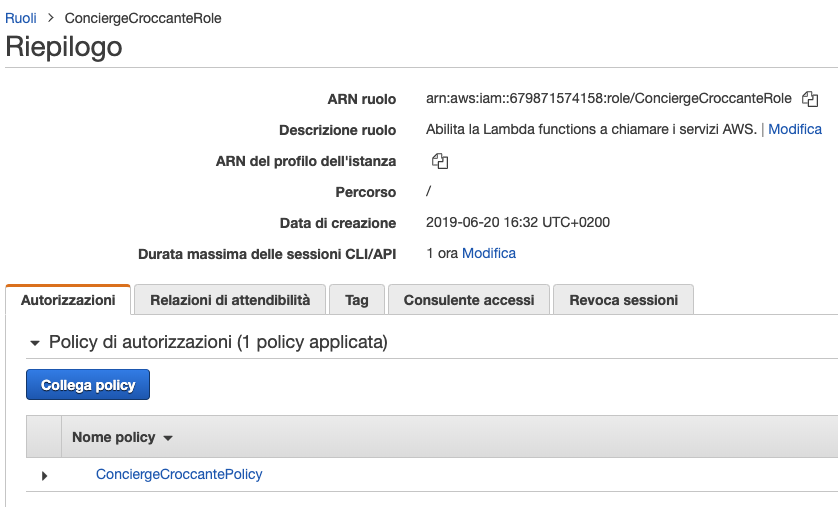
\includegraphics[width=1\columnwidth]{immagini/amazon-iam-role.png}
    \caption{\label{fig:esempio-amazon-iam-role}Esempio di Role creata}
\end{figure}

\newpage
\subsection{AWS CloudWatch}
Amazon CloudWatch\footnote{AWS CloudWatch. URL: \href{https://aws.amazon.com/it/cloudwatch/}{https://aws.amazon.com/it/cloudwatch/}} è un servizio di monitoraggio pensato per gli sviluppatori per fornire dati e analisi dal monitoraggio delle applicazioni, così da rispondere ai cambiamenti di prestazioni a livello di sistema, ottimizzare l'utilizzo delle risorse e ottenere una visualizzazione unificata dello stato di integrità operativa. CloudWatch raccoglie i dati di monitoraggio sotto forma di log, parametri ed eventi, unificando la loro visualizzazione, sulle applicazioni e i servizi eseguiti in AWS. Nel caso del progetto Concierce Croccante CloudWatch è stato utilizzato per rilevare comportamenti anomali della Skill, così da rilevare gli eventuali errori visualizzandone i log.
\begin{figure}[H] 
    \centering 
    
\includegraphics[width=0.8\columnwidth]{immagini/amazon-cloudwatch.png}
    \caption{\label{fig:icona_aws_cloudwatch}Icona AWS CloudWatch}
\end{figure}
\noindent Nel punto precedente, ovvero nel paragrafo \hyperref[aws-iam]{3.2.3}, è stato eseguito il procedimento necessario perché il servizio di CloudWatch venga abilitato. Pertanto non è necessario alcuna configurazione. Basterà recarsi al sito per poter utilizzare il servizio qualora si voglia visualizzare i dati sotto forma di log dopo o durante l'esecuzione di un servizio AWS, nel caso del progetto il servizio di AWS Lambda.

\subsection{AWS DynamoDB}
Amazon DynamoDB\footnote{AWS DynamoDB. URL: \href{https://aws.amazon.com/it/dynamodb/}{https://aws.amazon.com/it/dynamodb/}} è un servizio di database NoSQL (database non relazionale) proprietario e completamente gestito che supporta strutture di dati di tipo documento e di tipo chiave-valore. Caratteristiche di pregio sono database durevoli, multiregione e offrono sicurezza, backup, ripristino e cache in memoria per le applicazioni Internet. DynamoDB può gestire oltre 10 trilioni di richieste al giorno e supportando picchi di oltre 20 milioni di richieste al secondo. Nel progetto La Skill realizzata utilizza tale servizio per interrogare un database contenente la lista dei nomi del personale Crispy Bacon. 
\begin{figure}[H] 
    \centering 
    
\includegraphics[width=0.8\columnwidth]{immagini/amazon-dynamodb.png}
    \caption{\label{fig:icona_aws_dynamo}Icona AWS DynamoDB}
\end{figure}
\noindent È necessario quindi impostare tale servizio. Per farlo occorre recarsi nella pagina dedicata del db e una volta eseguito l'accesso con le proprie credenziali seguire le seguenti istruzioni:
\begin{itemize}
	\item Nel pannello a sinistra andare sulla sezione \texttt{Tabelle} e successivamente su \texttt{Crea Tabella}
	\item Nella nuova pagina sarà possibile settare le impostazioni della nuova tabella, quindi inserire un nome e due chiavi primarie, una di partizione e una di ordinamento, come mostra l'immagine seguente
	\begin{figure}[H] 
        \centering 
        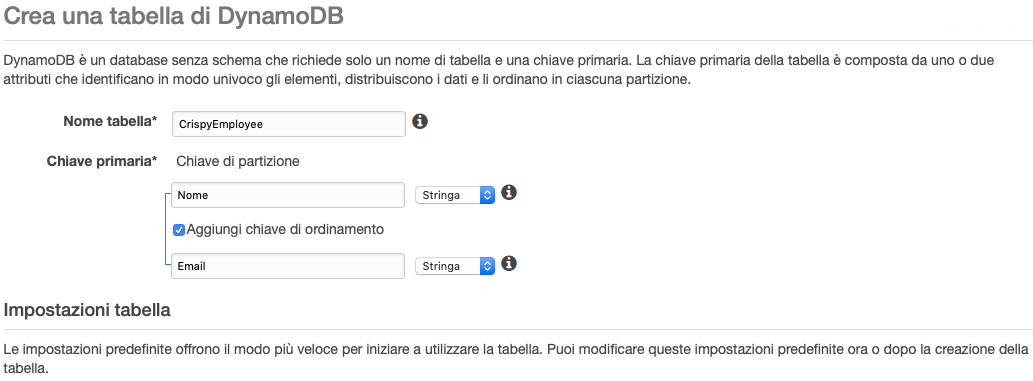
\includegraphics[width=1\columnwidth]{immagini/aws_dynamo.png}
	    \caption{\label{fig:esempio_aws_dynamo}Esempio creazione tabella AWS DynamoDB}
    \end{figure}
	
	\item Infine cliccare su \texttt{Crea}
\end{itemize}
Ora è possibile popolare il database inserendo i dati nell'apposito pannello di controllo di DynamoDB oppure fare delle interrogazioni da codice.

\newpage
\section{Creazione della Skill}
Una volta configurati correttamente tutti i servizi di AWS che Concierge Croccante andrà ad utilizzare si è proceduti con la realizzazione vera e propria della Skill. In questa parte infatti si andrà a mostrare e spiegare come questa sia stata realizzata basandosi sull'analisi della VUI fatta al punto \hyperref[vui]{2.5}. Il processo di realizzazione della Skill parte dalla console per sviluppatori di Alexa, a seguire la creazione della funzione Lambda dove verrà eseguito il programma, terminando infine con la stesura del codice mostrando parti di esso ritenute fondamentali. 
\subsection{Alexa Developer Console}
Per creare la Skill C.C. è necessario visitare ed entrare nella console di gestione ed accedere al servizio Alexa Skills Kit\footnote{Alexa Skill Kit. URL: \href{https://developer.amazon.com/it/alexa-skills-kit}{https://developer.amazon.com/it/alexa-skills-kit}}. Una volta fatto l’accesso con le proprie credenziali si è proceduto a creare il prodotto:
\begin{itemize}
	\item Cliccare su \texttt{Create Skill} per creare la Skill;\\
	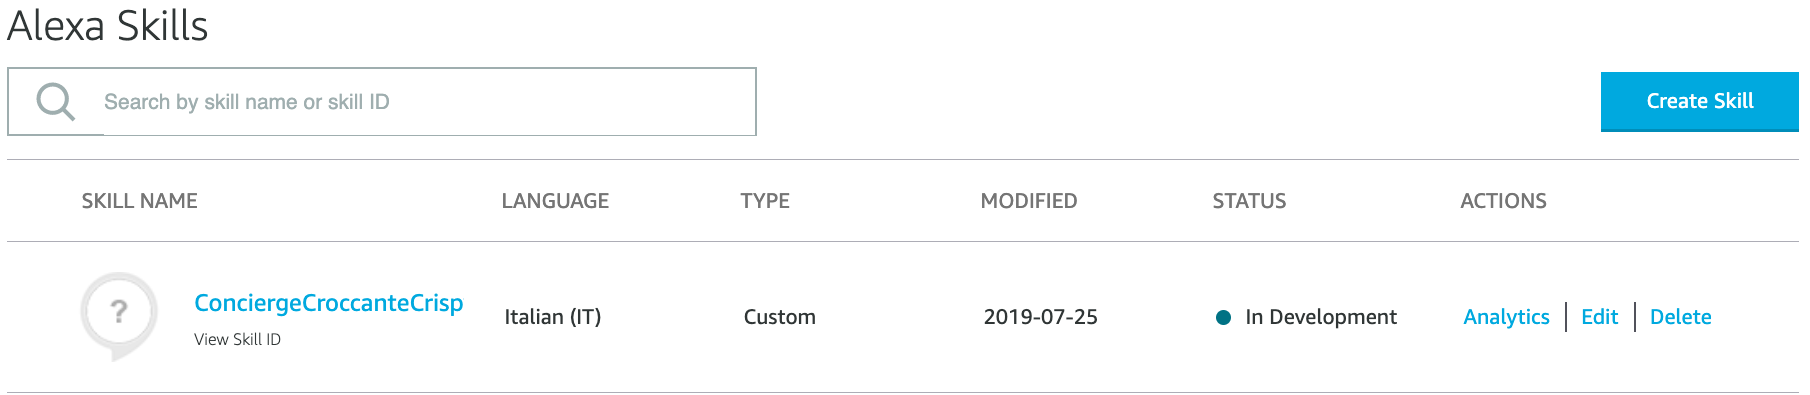
\includegraphics[width=12.5cm]{immagini/alexa-console-dev1.png}
	\item Nella pagina successiva, dare un nome alla propria Skill (facendo attenzione al fatto che quest'ultimo \textbf{non} sarà il nome di invocazione), scegliere la lingua, in questo caso \textit{Italian (IT)}, e scegliere \textit{Custom} come modello lasciando invariato il resto dei parametri. Successivamente cliccare nuovamente su \texttt{Create Skill};\\
	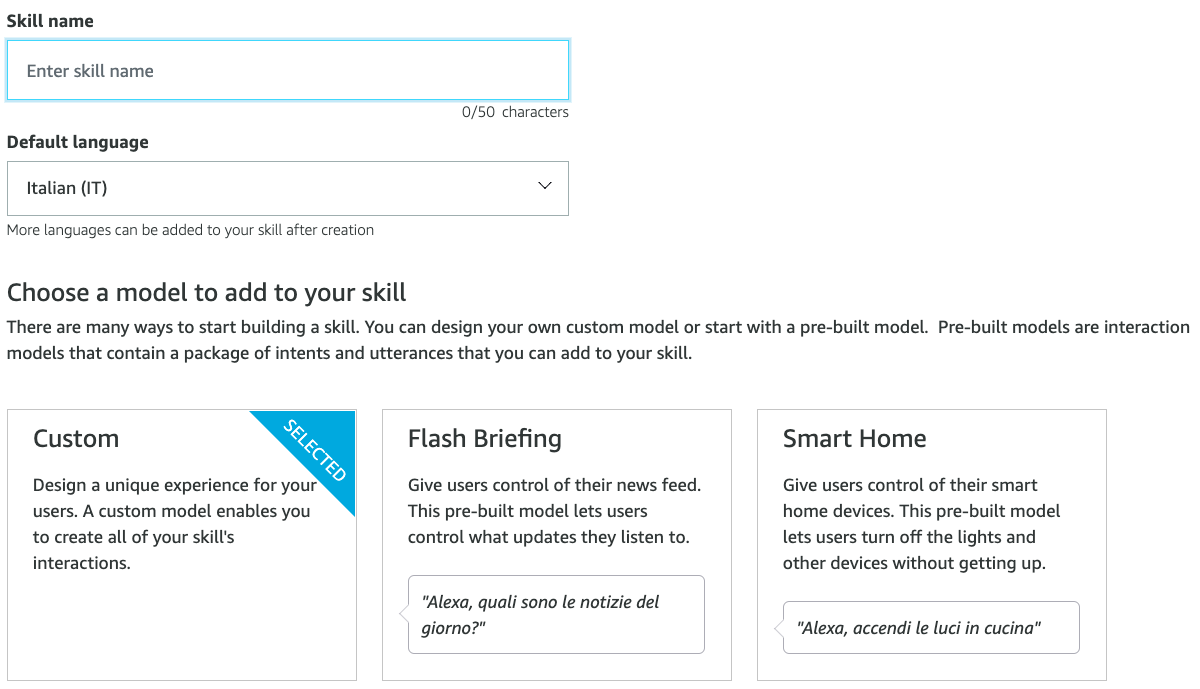
\includegraphics[width=13cm]{immagini/alexa-console-dev2.png}\\
	% 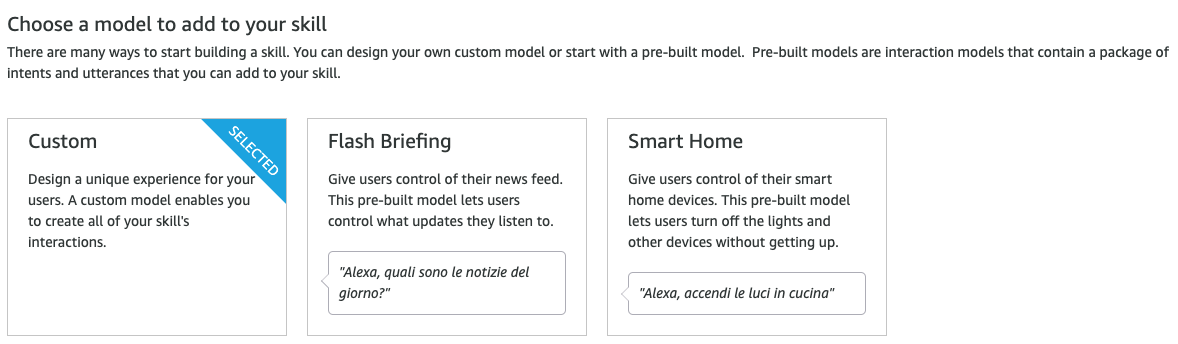
\includegraphics[width=12cm]{immagini/alexa-console-dev3.png}
	\newpage
	\item Si verrà reindirizzati nella pagina Alexa Developer Console dove sarà possibile customizzare la Skill. Nella sezione \texttt{Custom}, situata a sinistra, andare su \texttt{Invocation} per inserire il nome con cui si desidera invocare la Skill\\[0.5cm]
	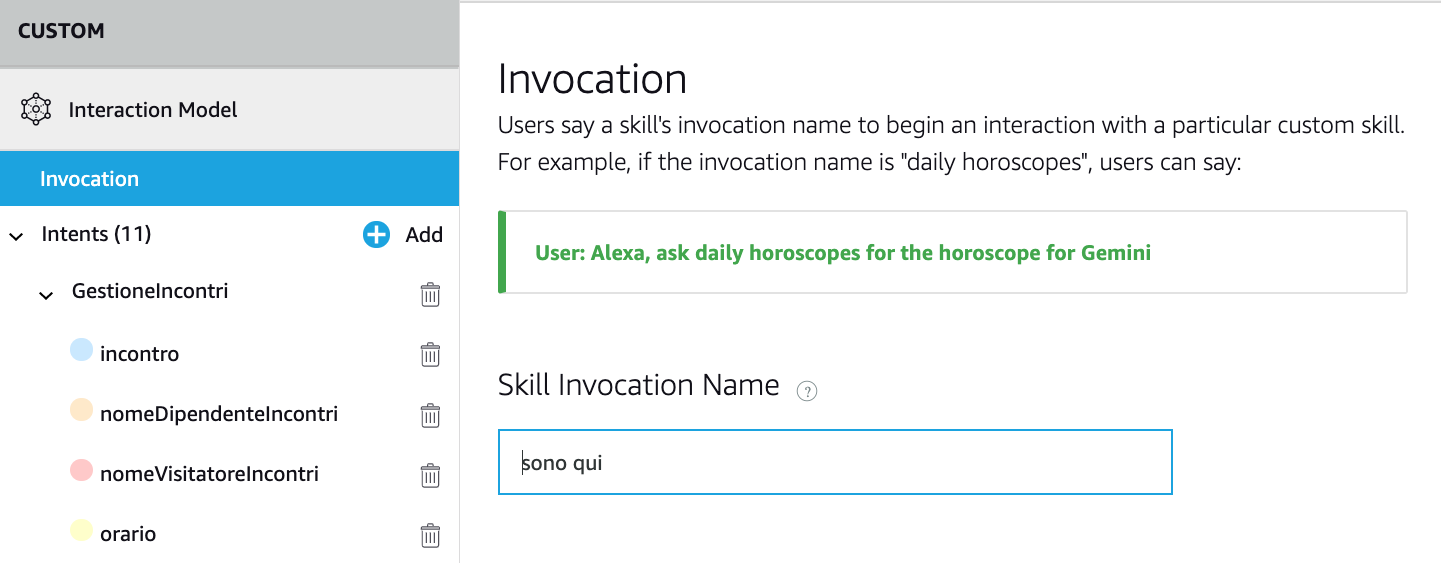
\includegraphics[width=12.5cm]{immagini/alexa-console-dev4.png}
	\item Successivamente è necessario creare gli intenti (\textit{intents}), che rappresentano un’azione che soddisfa una  richiesta del utente. Sempre nella sezione \texttt{Custom} - \texttt{JSON Editor} è possibile creari gli intenti caricando un file .json oppure scrivendoli sull'editor della pagina. A questo punto il comando di invocazione e gli intents sono stati impostati correttamente.\\[0.5cm]
	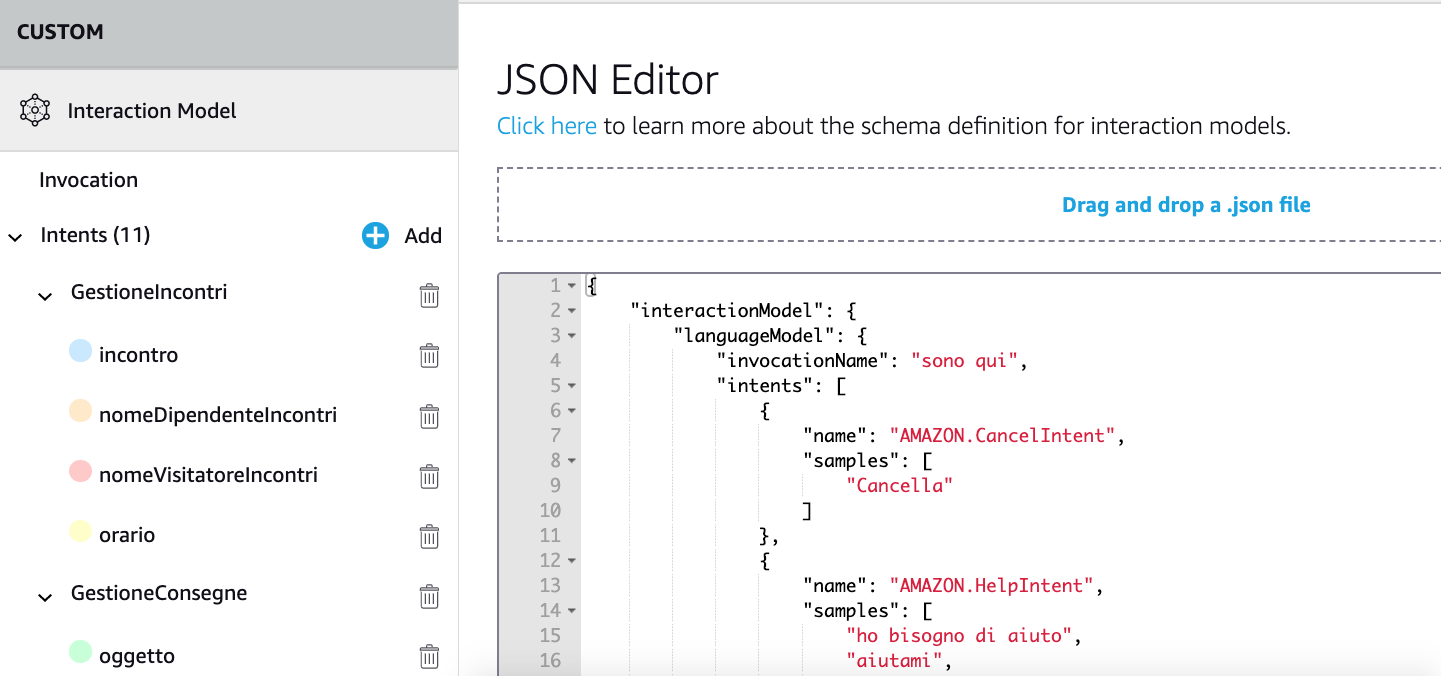
\includegraphics[width=12.5cm]{immagini/alexa-console-dev5.png}
\end{itemize}

\newpage
\noindent \subsubsection{Skill ID}
Il passo seguente è stato quello di salvare lo Skill ID, la chiave identificativa della Skill appena creata, che nei passi successi servirà per impostare l'endpoint: ovvero collegare la Skill alla Lambda dove risiederà il codice. Per fare ciò è stato sufficiente identificare e salvare l'ID inglobato nell'indirizzo URL della Skill appena creata, come mostra l'immagine seguente:
\begin{figure}[H]
	\centering
	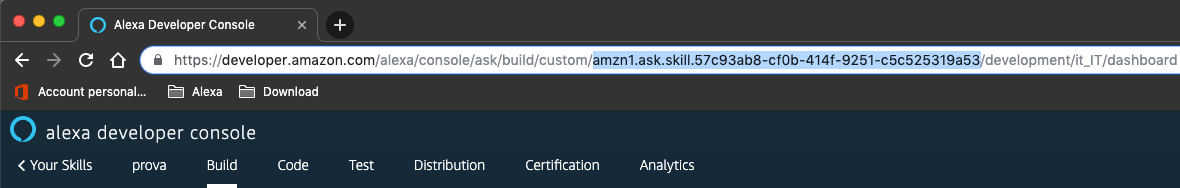
\includegraphics[width=13cm]{immagini/url_skill.png}
	\caption{Esempio Skill ID}
\end{figure}

\subsection{AWS Lambda}
Amazon Lambda\footnote{AWS Lamba. URL: \href{https://aws.amazon.com/it/lambda/}{https://aws.amazon.com/it/lambda/}} è un servizio della suite aws che consente di eseguire codice senza dover effettuare il provisioning\footnote{In telecomunicazioni è un servizi cloud a disposizione del utente che include hardware, software, cablaggio ed altro} e gestire server. Con Amazon Lambda è quindi possibile eseguire codice per qualsiasi tipo di applicazione o servizio back-end, senza alcuna amministrazione. Caricato il codice, Lambda attua tutte le azioni necessarie per eseguirlo e ricalibrare le risorse con massima disponibilità. È possibile anche configurare il codice in modo che venga attivato automaticamente da altri servizi AWS oppure che venga richiamato direttamente da qualsiasi applicazione Web o mobile.\\[0.5cm]
Una volta proceduti a creare la Skill la fese successiva è stata la realizzazione della funzione Lambda necessario per l'esecuzione del codice C.C.. Recandosi nell'omonima pagina, Amazon Lambda, sono stati eseguiti i passaggi di configurazione per creare la funzione ospitante il codice implementato o in fase di implementazione. Una volta fatto l'accesso con le proprie credenziali si è proceduto nel seguente modo:
\begin{minipage}{0.5\textwidth}
	\begin{figure}[H]
		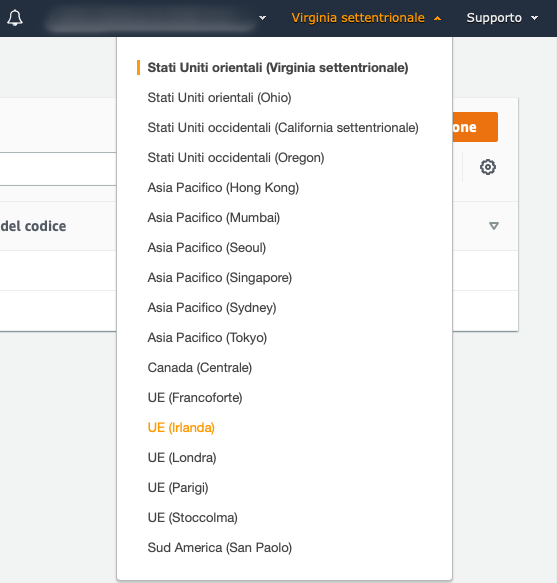
\includegraphics[width=6cm]{immagini/aws-lambda.png}
		\caption{\label{fig:aws_lambda_regione}Selezione regione AWS Lambda}
	\end{figure}
\end{minipage}
\begin{minipage}{0.5\textwidth}
	Prima di procedere è importate cambiare la regione di esecuzione della funzione Lambda. Quindi cliccare in alto a destra sulla regione (seconda voce) e scegliere \textit{UE (Irlanda)}, come mostrato in figura. Questo passaggio è necessario perché in base alla regione scelta, AWS - Lambda mette a disposizione più o meno servizi da integrare con la funzione. Tali informazioni possono essere reperite nell'apposita pagina\footnote{\href{https://amzn.to/30GkmTd}{https://amzn.to/30GkmTd}}. Di seguito viene fornito anche URL delle \href{https://amzn.to/2NCexm7}{Regioni ed endpoint AWS}\footnote{\href{https://amzn.to/2NCexm7}{https://amzn.to/2NCexm7}} dove sono riportate le informazioni degli endpoint di ogni servizio per ciascuna regione.
\end{minipage}
\begin{itemize}
	\item Cliccare in alto a destra su \texttt{Crea funzione} per creare la Lambda
	\item Nella pagina successiva, dare un nome alla funzione su cui verrà caricato il codice, nella sezione \texttt{runtime} scegliere \textit{Node.js 10.x} e infine nella sezione \texttt{Autorizzazioni} - \texttt{Ruolo di esecuzione} scegliere \textit{Utilizza ruolo esistente - ConciergeCroccanteRole} (ruole creato in precedenza durante la configurazione di AWS IAM al punto \hyperref[aws-iam]{3.2.3}). L'immagine seguente mostra la scelta corretta delle impostazioni base.\\[0.3cm]
	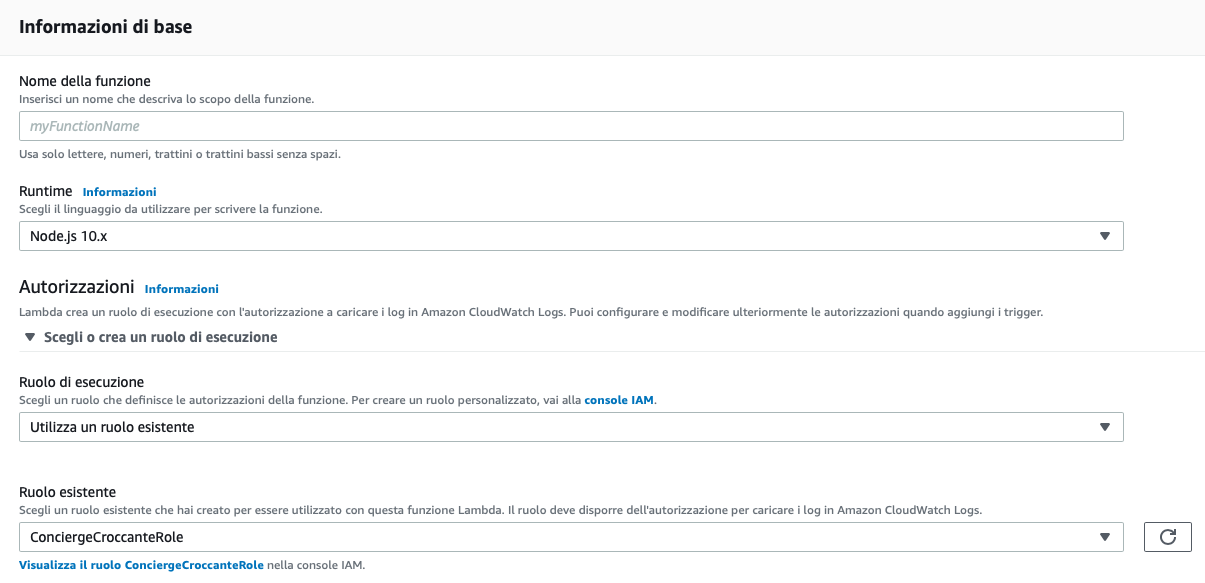
\includegraphics[width=13cm]{immagini/aws-lambda2}
	\item Successivamente cliccare nuovamente su \texttt{Crea funzione}
	\item Ora la funzione è stata impostata con le autorizzazioni sufficienti e necessarie per poter utilizzare i servizi che la Skill necessita. A destra cliccare su \texttt{Aggiungi trigger}, selezionare \texttt{Alexa Skill Kit}, inserire la Skill ID (salvata in precedenza) e cliccare su \texttt{Aggiungi} 
\end{itemize}
\subsubsection{Endpoint}
\label{endpoint}
Ora è possibile terminare il processo di configurazione della Skill eseguendo il collegamento tra Skill e Lambda. Ritornando nella console di AWS, sul servizio Lambda, è stato copiato l'indirizzo ARN della funzione, situato in alto a destra, come mostra nell'immagine seguente:
\begin{figure}[H]
	\centering
	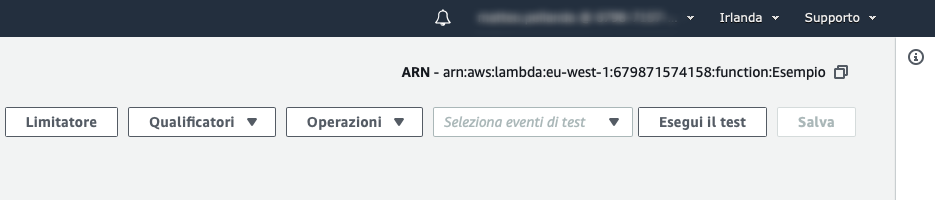
\includegraphics[width=13cm]{immagini/aws-lambda3.png}
	\caption{Esempio URL ARN Lambda}
\end{figure}
\noindent Successivamente, nella Skill in Alexa Developer Console, nella sezione \texttt{Custom} - \texttt{Endpoint}, incollare l'URL ARN della Lambda copiato in \texttt{Default Region}.
\begin{figure}[H]
	\centering
	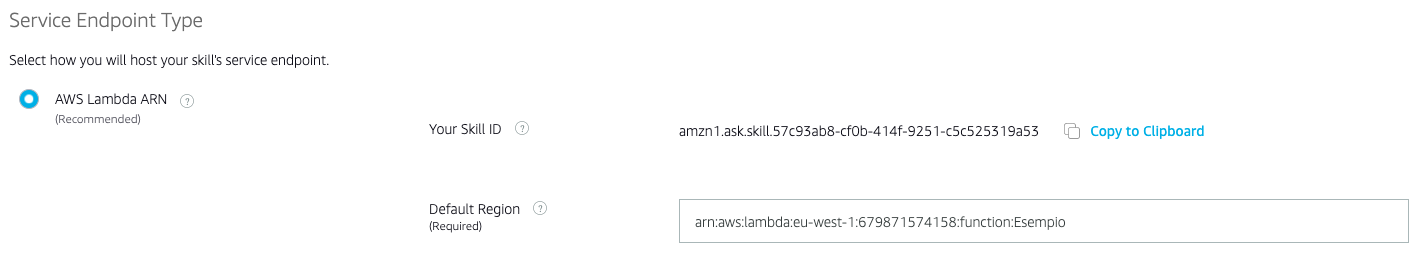
\includegraphics[width=13cm]{immagini/aws-lambda4.png}
	\caption{Esempio URL ARN Lambda}
\end{figure}
\noindent Infine cliccare su \texttt{Save Endpoint}. Ora la Skill l'endpoint impostato con l'esecuzione della funzione lambda creata.\\
Non rimane altro che caricare il codice del prodotto. Per farlo basterà recarsi nuovamente sulla console di AWS nel servizio Lambda, scegliere la propria funzione e su \texttt{Codice della funzione} scegliere \textit{Carica un file .zip} per caricare la cartella compressa del progetto.
\begin{figure}[H]
	\centering
	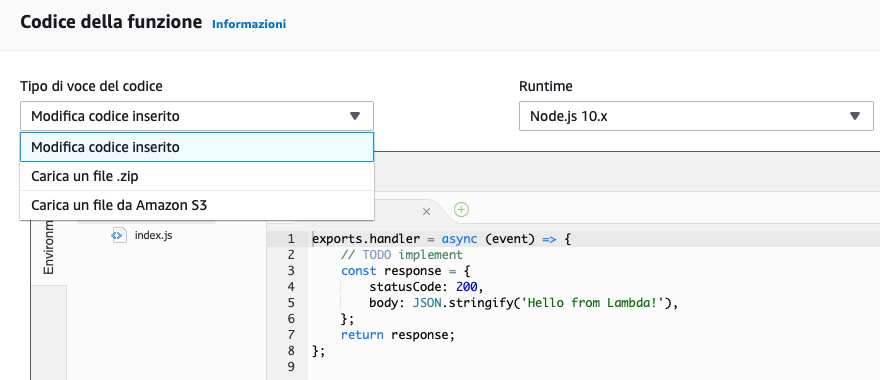
\includegraphics[width=13cm]{immagini/aws-lambda5.png}
	\caption{Codice funzione}
\end{figure}

\section{Organizzazione del codice}
Successiva alla parte di comprensione e configurazione dei servizi utilizzati in questo progetto, e alla creazione della Skill, è stato eseguito un micro-processo di organizzazione del codice prima della sua stesura. Questa pratica adottata è stata necessaria per avere uno schema e una gerarchia delle parti di codice che sono state sviluppate durante il periodo di tirocinio. Tale organizzazione ha permesso di sviluppare in maniera più ordinata e consapevole riducendo la probabilità di introdurre errori e rendendo il codice più manutenibile. Pertanto la cartella del progetto è stata così disposta:
\begin{itemize}
        \item \texttt{Skill}: cartella principale del progetto (main folder) contenente al suo interno altre cartelle e file organizzati secondo una determinata gerarchia
        \begin{itemize}
            \item[>] \texttt{apl-data}: cartella contenente i dati delle schermate APL
            \item[>] \texttt{apl-template}: cartella contenente i template lo stile delle schermate APL
            \item[>] \texttt{hendelrs}: cartella contenente i file .js di ogni handlers (gestori) creati nella Skill
            \item[>] \texttt{i18n}: cartella contente file .js con le traduzioni della lingua 
            \item[>] \texttt{node\_modules}: cartella contenente tutti i pacchetti installati con il gestore npm
            \item[>] \texttt{task}: cartella contente file .js da eseguire a riga di comando per l'esecuzione di funzionalità primitive 
            \item[>] \texttt{utils}: cartella contente file .js con classi di utilità, come lettura del db, invio di e-mail, ecc..
            \item[-] \texttt{credentials.json}: file contenente delle credenziali per accedere al servizio di Google Calendar
            \item[-] \texttt{googleAuthTokenCredential.json}: file contenente delle credenziali per accedere al servizio di Google Calendar
            \item[-] \texttt{index.js}: file principale dove inizia l'esecuzione della Skill. La Lambda difatti partirà con la lettura di questo file
            \item[-] \texttt{intent.json}: file .json contenente tutti gli intent creati per la Skill
            \item[-] \texttt{package.-lock.json}: file di configurazione automaticamente creato dal gestore di pacchetti npm
            \item[-] \texttt{package.json}: file di configurazione automaticamente creato dal gestore di pacchetti npm
            \item[-] \texttt{policy.json}: file .json contente le regole di policy create al punto \hyperref[aws-iam]{3.2.3}
        \end{itemize}
    \end{itemize}
\begin{figure}[H]
	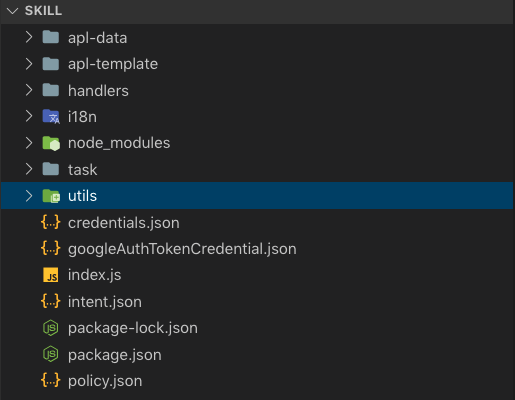
\includegraphics[width=13cm]{immagini/skill-folder.png}
	\caption{\label{fig:gerarchia_cartella_cc}Gerarchia cartella progetto C.C.}
\end{figure}

\subsection{Handlers}
Come descritto prima la cartella del progetto C.C. è stata disposta per una gestione ordinata del codice. Una delle sotto-cartelle contenute al suo interno è dedicata per la gestione degli handelrs. Nel codice della Skill gli handerls sono delle funzioni che hanno lo scopo di gestire gli intenti che vengono scatenati all'invocazione di un comando da parte dell'utente. Gli handlers sono stati così realizzati:
\begin{itemize}
    \item \texttt{index.js}: che contiene ed ingloba l'export di tutte le classi dei handlers contenuti in questa cartella
    
    \item \texttt{gestioneConsegne\_Complete.js}: questo handler ha il compito di catturare l'evento nel caso in cui l'utente intenda consegnare un pacco (o lettera) sapendo già il nome del destinatario e, o l'oggetto consegnato o la professione dell'utente che sta conversando
    \item \texttt{gestioneConsegne\_NomeDipendete.js}: questo handler ha il compito di catturare l'evento nel caso in cui l'utente intenda consegnare un pacco (o lettera) senza sapere già il nome del destinatario. Questo gestore ha il compito di richiedere tale dato domandandolo all'utente che sta conversando con la Skill
    \item \texttt{gestioneIncontri\_Complete.js}: questo handler ha il compito di catturare l'evento nel caso in cui l'utente visitatore abbia un appuntamento e i dati necessari sono stati tutti raccolti
    \item \texttt{gestioneIncontri\_NomeDipendente\_NomeVisitatore.js}: questo handelr ha il compito di catturare l'evento nel caso in cui l'utente visitatore abbia un appuntamento e, il nome del dipendetene cercato e del cliente appena entrato, sono stati raccolti. Il gestore eseguirà dei controlli per verificare l'attendibilità dei dati per poi proseguire con il dialogo oppure chiedendone di nuovi dati
    \item \texttt{gestioneIncontri\_NomeDipendente.js}: questo handler ha il compito di catturare l'evento nel caso in cui l'utente abbia un appuntamento e la Skill richiede il nome del dipendente cercato
    \item \texttt{gestioneIncontri\_Orari.js}: questo handler ha il compito di catturare l'evento nel caso in cui l'utente abbia un appuntamento e la Skill richiede l'orario per verificare l'evento nel calendario
    \item \texttt{vorreiIncontri\_Complete.js}: questo handler ha il compito di catturare l'evento nel caso in cui l'utente visitatore desideri incontrare un dipendente e sono stati raccolti tutti i dati necessari 
    \item \texttt{vorreiIncontri\_CompleteWithOrario.js}: questo handler ha il compito di catturare l'evento nel caso in cui l'utente visitatore desideri incontrare un dipendente e richiede l'orario di appuntamento per verificare l'esistenza dell'evento nel calendario 
    \item \texttt{vorreiIncontri\_NomeDipendente\_NomeVisitatore.js}: questo handler ha il compito di catturare l'evento nel caso in cui l'utente visitatore desideri incontrare un dipendente e, il nome del dipendetene cercato e del cliente appena entrato, sono stati raccolti. Il gestore eseguirà dei controlli per verificare l'attendibilità dei dati per poi proseguire con il dialogo oppure chiedendone di nuovi dati
    \item \texttt{vorreiIncontri\_NomeDipendente.js}: questo handler ha il compito di catturare l'evento nel caso in cui l'utente visitatore desideri incontrare un dipendente e la Skill richiede il nome di quest'ultimo
    \item \texttt{vorreiIncontri\_SiNo.js}: questo handler ha il compito di catturare l'evento nel caso in cui l'utente visitatore abbia un appuntamento e la Skill ne richiede l'orario per verificare l'evento nel calendario
    \item \texttt{touchWrapperUserEvent.js}: questo handler ha il compito di catturare gli eventi scatenati dal tocco sul display 
\end{itemize}
\begin{figure}[H]
	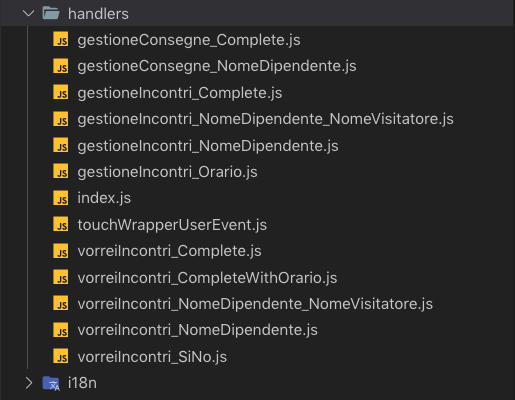
\includegraphics[width=13cm]{immagini/skill-folder2.png}
	\caption{\label{fig:gerarchia_cartella_cc2}Gerarchia cartella progetto C.C. - Handlers}
\end{figure}
\subsection{Utils}
\label{utils}
Lo stesso criterio usato per gli handlers è stato adotta anche per le classi Javascript che contengono il codice delle funzionalità della Skill. La cartella \textit{utils} contiene appunto quei metodi che permetto ad esempio la lettura del databse, l'invio di e-mail, l'invio di notifiche e la lettura del calendario. Le utilità sono state così realizzate:
\begin{itemize}
    \item \texttt{databaseUtils.js}: questa classe mette a disposizione i metodi per interrogare il database e sono presenti le seguenti funzioni:
    \begin{itemize}
        \item[>] \texttt{getInstance()}
        \item[>] \texttt{runQuery(params: var)}
        \item[>] \texttt{runScan(params: var)}
        \item[>] \texttt{runPut(params: var)}
        \item[>] \texttt{checkEmployee(nome\_dipendente: var)}
    \end{itemize}
    \item \texttt{emailUtils.js}: questa classe mette a disposizione i metodi per l'invio di messaggi e-mail ed è presente la seguente funzione:
    \begin{itemize}
        \item[>] \texttt{sendMail(from: var, to: var, message: var, oggetto: var)}
    \end{itemize}
    \item \texttt{gcalendarUtils.js}: questa classe mette a disposizione i metodi per la lettura e verifica di eventi nel calendario e sono presenti le seguenti funzioni:
    \begin{itemize}
        \item[>] \texttt{listEvents(idCalendar: var)}
        \item[>] \texttt{checkEvent(events: var, email\_dipendente: var, nome\_visitatore: var, orarioEvento: var)}
        \item[>] \texttt{generateOAuth2Client()}
    \end{itemize}
    \item \texttt{gchatUtils.js}: questa classe mette a disposizione i metodi per l'invio di notifiche su Google Chat, funzionalità in fase di sviluppo fatta nell'ultimo periodo di tirocinio, e sono presenti le seguenti funzioni:
    \begin{itemize}
        \item[>] \texttt{sendNotify(type: var, message: var)}
        \item[>] \texttt{checkThread(type: var)}
        \item[>] \texttt{putThread(thread: var, thread\_type: var)}
    \end{itemize}
    \item \texttt{prepareQuery.js}: questa classe mette a disposizioni i metodi per ricevere le query di interrogazione che si desidera e sono presenti le seguenti funzioni:
    \begin{itemize}
        \item[>] \texttt{scanEmployee()}
        \item[>] \texttt{queryEmployee(nomeDipendente: var)}
        \item[>] \texttt{putThread()}
        \item[>] \texttt{updateThread(old\_thread: var, new\_thread: var)}
    \end{itemize}
    \item \texttt{slacknotifyUtils.js}: questa classe mette a disposizione i metodi per l'invio di notifiche su Slack e al suo interno sono presenti le seguenti funzioni:
    \begin{itemize}
        \item[>] \texttt{sendNotify(channel: var, message: var)}
        \item[>] \texttt{sendDirectlyNotify(member: var, MESSAGE: var)}
        \item[>] \texttt{addTag(toTag: var)}
        \item[>] \texttt{listMembersApl(intent: var)}
        \item[>] \texttt{getIdMember(toTag: var)}
        \item[>] \texttt{membersList()}
    \end{itemize}
    \item \texttt{abracadabraUtils.js}: questo metodo contiene un easter egg\footnote{Un easter egg in informatica è un contenuto di natura bizzarra e innocuo che gli sviluppatori nascondono all'interno del prodotto}
\end{itemize}
\begin{figure}[H]
	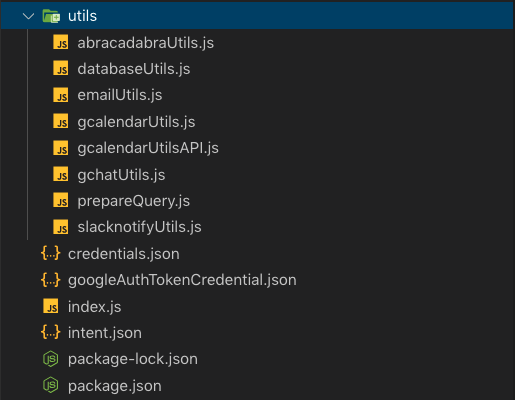
\includegraphics[width=13cm]{immagini/skill-folder3.png}
	\caption{\label{fig:gerarchia_cartella_cc3}Gerarchia cartella progetto C.C. - Utils}
\end{figure}

\section{Pacchetti}
Particolare attenzione va fatta sulla gestione dei pacchetti e quali di essi sono stati installati nel progetto Concierge Croccante. A tale necessità è stato utilizzato il gestore di pacchetti npm, menzionato in precedente al punto \hyperref[npm]{1.5.4}, che ha consentito di installare in maniera sicura e immediata i pacchetti necessari. Installando tali pacchetti il gestore ha suddiviso il codice all'interno di una directory chiamata \texttt{node\_modules} creando inoltre un file di configurazione delle installazioni fatte.
\begin{figure}[H]
	
\includegraphics[width=12cm]{immagini/logo-npm.png}
	\caption{\label{fig:logo_npm}Logo NPM}
\end{figure}
\noindent In questa fase di progetto si è provveduto ad installare npm e tutti i pacchetti necessari alla Skill Concierge Croccante nel seguente modo:
\begin{itemize}
    \item Dalla documentazione di npm\footnote{Doc npm. URL: \href{https://docs.npmjs.com/downloading-and-installing-node-js-and-npm}{https://docs.npmjs.com/downloading-and-installing-node-js-and-npm}} viene riportato il seguente comando da eseguire su terminale:
    \begin{lstlisting}[language=bash]
		$ [sudo] npm install npm -g
	\end{lstlisting}
	Il comando installerà l'ultima versione del gestore pacchetti. Se si desidera verificare e visualizzare l'ultima versione di npm è necessario eseguire il comando: 
	\begin{lstlisting}[language=bash]
		$ npm -v
	\end{lstlisting}
	\item I pacchetti installati nel progetto sono stati i seguenti:
	\begin{itemize}
	    \item[>] \texttt{ask-sdk} e \texttt{ask-sdk-core} di AWS che semplifica la creazione di Skill, permettendo di utilizzare le funzionalità base di Alexa in maniera rapida:
	    \begin{lstlisting}[language=bash]
		    $ npm install --save ask-sdk
		    $ npm install --save ask-sdk-core
	    \end{lstlisting}
	    \item[>] \texttt{request} per semplificare ed effettuare chiamate http, supporta HTTPS i re-indirizzamenti:
	    \begin{lstlisting}[language=bash]
		    $ npm install request
	    \end{lstlisting}
	    \item[>] \texttt{googleapis} è una libreria client per l'utilizzo delle API di Google, rendendo più semplice ed immediate le chiamate ai servizi come Calendar:
	    \begin{lstlisting}[language=bash]
		    $ npm install googleapis
	    \end{lstlisting}
	    \item[>] \texttt{slack-notify} è una libreria che rende flessibile l'utilizzo dell'API Webhooks\footnote{Incoming Webhooks. URL: \href{https://api.slack.com/incoming-webhooks}{https://api.slack.com/incoming-webhooks}} di Slack, semplificando l'invio di notifiche a Slack dalla Skill:
	    \begin{lstlisting}[language=bash]
		    $ npm install slack-notify
	    \end{lstlisting}
	    \item[>] \texttt{i18next} e \texttt{i18next-sprintf-postprocessor} sono dei framework di internazionalizzazione popolari ambienti javascript:
	    \begin{lstlisting}[language=bash]
		    $ npm install i18next
		    $ npm install i18next-sprintf-postprocessor
	    \end{lstlisting}
	\end{itemize}
\end{itemize}

\newpage
\section{Calendario}
Per la soddisfazione del requisito RO17 analizzato al punto \hyperref[requisti-richiesti]{2.3}, ovvero la lettura e verifica degli appuntamenti in calendario, è stato richiesto l'uso di Google Calendar, giù utilizzato dall'azienda Crispy Bacon per le sue note funzionalità. 
\subsection{Google Calendar}
Per l’integrazione col servizio di Google Calendar sono a disposizione delle API documentate reperibili al indirizzo \href{https://developers.google.com/calendar/}{developers.google.com/calendar/}. Dalla guida emergono i seguenti requisti necessari:\\
\begin{minipage}{0.5\textwidth}
	\begin{figure}[H]
		
\includegraphics[width=5cm]{immagini/google_calendar.png}
		\caption{\label{fig:icona_google_calendar}Icona Google Calendar}
	\end{figure}
\end{minipage}
\begin{minipage}{0.5\textwidth}
	\begin{itemize}
		\item Node.js
    	\item googleapis package
    	\item Account Google funzionante e verificato
    	\item Autorizzazione OAuth\footnote{OAuth: protocollo di rete open e standard, progettato per lavorare con il protocollo HTTP.}
	\end{itemize}
\end{minipage}
\\[0.5cm]
Nei punti successivi verranno analizzati aspetti importanti, con esempi di codice, riguardante l'integrazione con il calendario in questione e l’uso delle sue API.
\subsubsection{OAuth2}
Per consentire la lettura ed ottenere la lista di eventi presenti nel calendario è stato necessario eseguire un'autenticazione tramite il protocollo OAuth 2.0\footnote{OAuth 2.0. URL: \href{https://oauth.net/2/}{https://oauth.net/2/}}. Quest'ultimo è un protocollo di rete open che consente l'emissione di un token di accesso da parte di un server autorizzato ad un client di terze parti, nel nostro caso il servizio di Google Calendar, previa approvazione dell'utente proprietario della risorsa cui si intende accedere. Per poter ottenere ciò sono stati svolti i seguenti passi:
\begin{itemize}
    \item Visitando la pagina Google Calendar API\footnote{G. Calendar API. URL: \href{https://developers.google.com/calendar/quickstart/nodejs}{https://developers.google.com/calendar/quickstart/nodejs}} è stato abilitato l'utilizzo delle API per il calendario. Nella pagina infatti è presente il primo step da seguire dal titolo ”\textit{Turn on the Google Calendar API}” dove presente il bottone adibito all'abilitazione:\\
    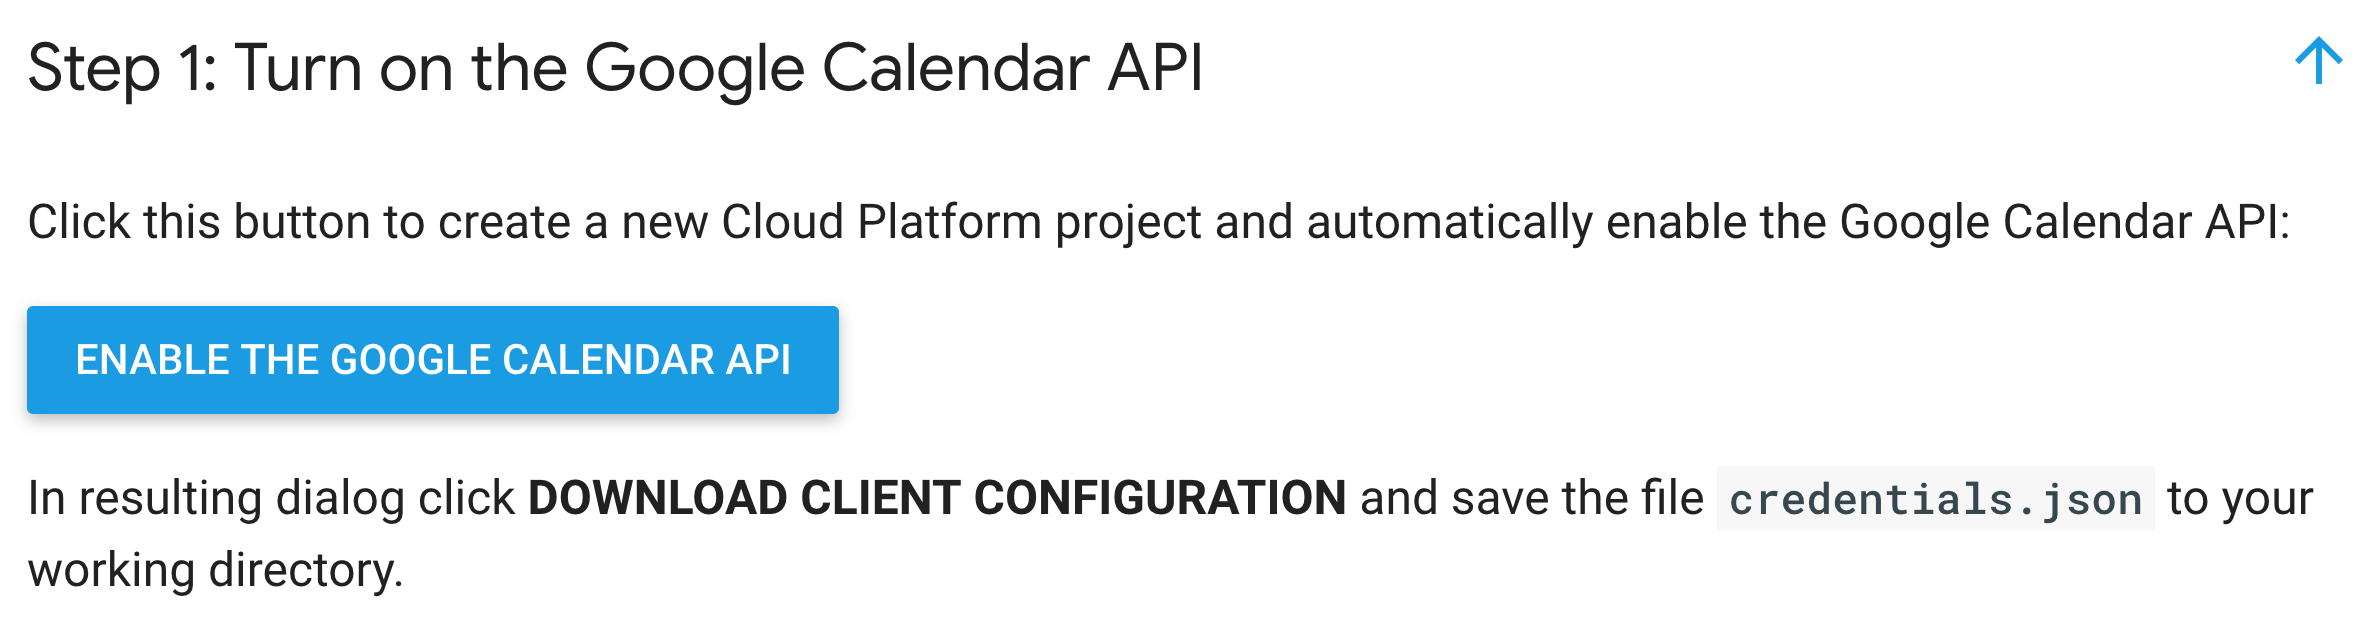
\includegraphics[width=12cm]{immagini/google_calendar_api.png}\\[2cm]
    Nella sezione corrente, una volta cliccato il bottone \texttt{ENABLE THE GOOGLE CALENDAR API} ed eseguito l’accesso con l’account Google il quale si desidera leggere gli eventi in calendario, è stato salvato il file credentials.json ottenuto dall'accesso e fornito nella cartella di progetto.
    \item Sempre nella stessa pagina è stato copiato ed eseguito l'esempio di set up riportato per ottenere l’OAuth necessario a visualizzare gli eventi nel calendario. Di seguito si riporta tale esempio di codice, importante appunto per ricevere le autorizzazioni necessarie:
	\lstinputlisting[caption=Esempio Set up Google Calendar]{code/generateGoogleAuthToken.js}
	\item Per eseguire tale esempio di codice è stato sufficiente aprire il terminale sulla cartella di progetto dove risiede il file di set up e lanciare lo script con il seguente comando:
	\begin{lstlisting}[language=bash]
		$ node [filename]
	\end{lstlisting}
	Nel caso in cui fossa la prima volta che eseguito tale esempio è necessario autorizzare l'accesso:
	\begin{enumerate}
		\item Aprire l'URL restituito dal terminale col proprio web browser
		\item Fare il login in se non si è già loggati
		\item Cliccare il bottone \texttt{Accept}
		\item Copiare il codice ricevuto, incollarlo nella terminale e premere \texttt{Enter}
	\end{enumerate}
\end{itemize}
\subsubsection{Lettura eventi}
All'interno del progetto Concierge Croccante la fase di lettura del calendario è stata semplificata realizzando una classe contenente al suo interno metodi appositi. Di tali metodi, già menzionati al punto \hyperref[utils]{3.4.2}, ne viene riportato il codice e analizzato il loro funzionamento:
\lstinputlisting[caption=Metodi listEvent e generateOAuth2Client]{code/gcalendarUtils1.js}
Per ottenere la lista di eventi non servirà altro che richiamare \texttt{listEvents(idCalendar)}. La funzione ritornerà un oggetto contenente tutti gli eventi, con le loro informazioni, della giornata odierna fino ad un massimo di 15 risultato. Attenzione: i file citati credentials.json e googleAuthTokenCredential.json non sono altro che le credenziali recuperate nei punti precedenti per accedere con il token OAuth.
\\[0.5cm]
Altro metodo presente e largamente utilizzato è \texttt{checkEvent(events, email\_dipendente, nome\_visitatore, orarioEvento)}:
\lstinputlisting[caption=Metodo checkEvent]{code/gcalendarUtils2.js}
Questo metodo pone come precondizione il fatto di ricevere in ingresso l'elenco di eventi ed i valori: nome visitatore, nome persona cercata ed orario; non vuoti. Il risultato sarà un valore \textit{boolean false} nel caso \textbf{non} sia presente alcun evento nel calendario, un valore numerico \textit{1} nel caso sia stato trovato un evento per la persona e l'orario indicato, oppure \textit{0} se esiste un evento ma l'orario indicato non coincide con quello effettivo.

\newpage
\section{Invio notifiche}
Altra specifica per la soddisfazione dei requisiti RO18 e RO19 analizzati al punto \hyperref[requisti-richiesti]{2.3}, è l'invio di notifiche. Per ovviare a ciò sono state realizzate le funzionalità per l'invio di messaggi istantanei via Slack e e-mail via AWS SES visto il già utilizzo di questi servizi da parte di Crispy Bacon.
\subsection{Slack}
Per l’integrazione col servizio di Slack sono a disposizione delle API documentate reperibili al indirizzo \href{https://api.slack.com/}{api.slack.com/}. Dalla guida emergono i seguenti requisti necessari:
\\
\begin{minipage}{0.5\textwidth}
	\begin{figure}[H]
		
\includegraphics[width=6cm]{immagini/slack.png}
		\caption{\label{fig:icona_slack}Icona servizio - Slack}
	\end{figure}
\end{minipage}
\begin{minipage}{0.5\textwidth}
	\begin{itemize}
		\item Node.js
		\item slack-notify package
		\item Account Slack
		\item Incoming Webhook
	\end{itemize}
\end{minipage}
\\[0.4cm]
Nei punti successivi verranno analizzati aspetti importanti, con esempi di codice, riguardante l'invio di notifiche con Slack e l’uso delle sue API.
\subsubsection{Incoming Webhooks}
Per consentire l'invio di messaggi di notifica via chat viene scelto di utilizzare un bot con Incoming Webhook\footnote{\href{https://it.wikipedia.org/wiki/Webhook}{https://it.wikipedia.org/wiki/Webhook}}. Quest'ultimo è un mezzo con il quale si semplifica l'invio di messaggi da un'applicazione a Slack. La creazione di un Incoming Webhook fornisce un URL univoco a cui si invia un payload JSON con il testo del messaggio e alcune opzioni.
Per ottenere l'Incoming Webhook sono stati eseguiti i seguenti passaggi:
\begin{itemize}
    \item Visitando la pagina dedicata \href{https://api.slack.com/incoming-webhooks}{api.slack.com/incoming-webhooks} è stata creata un'App per Slack cliccando sul bottone \texttt{"Create your Slack app"}:\\
    
\includegraphics[width=12cm]{immagini/slack_bot.png}\\
    Si viene successivamente indirizzati in una nuova pagina dove sarà possibile creare la propria App per Slack:
	\begin{enumerate}
		\item Cliccare sul bottone \texttt{Create New App}
		\item Inserire il nome dell'app
		\item Scegliere lo \textit{space} di lavoro dove installare l'app
		\item Cliccare su \texttt{Crea App}
	\end{enumerate}
	\item Dopo aver creato l'App è stato abilitato l'Incoming Webhook nell'apposita pagina delle impostazioni. Fatto sono state visualizzate alcune opzioni aggiuntive. Tra queste era presente il pulsante \textit{Aggiungi nuovo Webhook a Workspace}. Viene quindi aggiunto il Webhook ad canale/space di Slack designato per pubblicare l'App e salvata tale modifica facendo clic su \texttt{Autorizza la tua app}.
\end{itemize} 
\subsubsection{Invio notifiche}
All'interno del progetto Concierge Croccante la fase di notifica via Slack è stata semplificata realizzando una classe contenente al suo interno metodi appositi. Di tali metodi menzionati al punto \hyperref[utils]{3.4.2} ne viene riportato il codice e analizzato il loro funzionamento\footnote{NB: la variabile \texttt{MY SLACK WEBHOOK URL} contiene l'URL del Webhook dell'App}: 
\lstinputlisting[caption=Metodo sendNotify]{code/slacknotifyUtils1.js}
Il codice sopra riportato mostra il metodo \texttt{sendNotify(channel:  var, message:  var)}: tale funzione non fa altro che inviare il testo del messaggio nel canale di Slack desiderato passando i dati per parametro. La variabile constante \texttt{slack.send} richiama il metodo fornito del pacchetto \texttt{slack-notify} che non farà altro che fare una \textit{request} in \textit{POST} all'API \texttt{chat.postMessage}. Nel caso in cui il metodo riscontrasse un errore nell'invio del messaggio viene lanciata un eccezione.

\newpage
\lstinputlisting[caption=Metodo sendDirectlyNotify]{code/slacknotifyUtils2.js}
Per l'invio delle notifiche in direct message\footnote{Messaggio privato inviato in un social media} è stato messo a disposizione il metodo \texttt{sendDirectlyNotify(member:  var, MESSAGE:  var)}: tale funzione invierà il testo del messaggio al destinatario indicato alla funzione facendo, anche in questo caso, una \textit{request} in \textit{POST} all'API \texttt{chat.postMessage}. Differentemente dal metodo precedente qui non viene utilizzata alcuna libreria, ma viene usata l'API in maniera diretta.

\newpage
\lstinputlisting[caption=Metodo addTag]{code/slacknotifyUtils3.js}
Altra funzionalità messa a disposizione dalla classe è il metodo \texttt{addTag(toTag: var)}: tale funzione non fa altro che richiamare una funzione ausiliaria e privata della classe, più elaborata e non visibile all'utente esterno, che va ad aggiungere, grazie all'id del membro cercato, il tag necessario per menzionarlo all'interno delle chat di gruppo.

\newpage
\lstinputlisting[caption=Metodo listMembersApl]{code/slacknotifyUtils4.js}
Metodo più rilevante è \texttt{listMembersApl(intent: var)}: tale metodo viene richiamato dalla Skill qualora è necessaria la costruzione di un APL con elementi touch che al momento del tocco scatenino un evento. In questo caso l'APL che si va a creare è una lista dei membri di Crispy Bacon dove è possibile selezionare il nome per fornirlo alla Skill. 

\newpage
\subsection{E-mail}
Per l'invio di notifiche via e-mail, come già detto in precedenza, è stato utilizzato il servizio Amazon SES e la sua integrazione con il servizio sono necessari i seguenti requisiti:
\\
\begin{minipage}{0.47\textwidth}
	\begin{figure}[H]
		
\includegraphics[width=6cm]{immagini/ses.png}
		\caption{\label{fig:google_calendar}Icona servizio - SES}
	\end{figure}
\end{minipage}
\begin{minipage}{0.5\textwidth}
	\begin{itemize}
		\item Node.js
		\item npm aws-sdk
		\item Account AWS
		\item Indirizzo e-mail
	\end{itemize}
\end{minipage}
\\[0.4cm]
Nei punti successivi verranno analizzati aspetti importanti, con esempi di codice, riguardante l'invio di e-mail con Amazon SES e l'uso della libreria SDK.

\subsubsection{Invio e-mail}
All'interno del progetto Concierge Croccante l'invio di notifiche o messaggi via e-mail è stata semplificata realizzando una classe contenente al suo interno metodi appositi. Di tali metodi menzionati al punto \hyperref[utils]{3.4.2} ne viene riportato il codice e analizzato il loro funzionamento: 

\lstinputlisting[caption=Metodo sendMail]{code/emailUtils.js}
Il codice sopra riportato mostra il metodo \texttt{sendMail(from:  var, to:  var, message:  var, oggetto:  var)}: tale funzione non fa altro che inviare una e-mail con i campi from, to, message ed oggeto passati per parametro. La variabile constante \texttt{ses} non fa altro che richiamare il metodo fornito del pacchetto \texttt{aws-sdk} che si occuperà di richiamare le API necessarie all'utilizzo di AWS SES.

\newpage
\section{Lettura del Database}
Funzionalità a supporto di quelle principali è la lettura del database DynamoDB. Quest'ultimo è popolato da una tabella contente i nomi di tutti i dipendenti dell'azienda Crispy Bacon, i quali, vengono prelevati per essere utilizzati nelle fasi di controllo, come la ricerca di un dipendente per verificarne la sua esistenza. Il progetto predispone due classi adibite a questo tipo di funzionalità per interrogare il database: \texttt{databaseUtils.js} e \texttt{prepareQuery.js}.

\lstinputlisting[caption=Metodo getInstance e runQuery]{code/databaseUtils.js}
Il codice sopra riportato mostra la classe coi metodi per eseguire \textit{query} di diversa tipologia: \texttt{runQuery(params:  var)} non fa altro che richiamare il metodo presente nel pacchetto \texttt{aws-sdk} per l'esecuzione di un interrogazione standard. Altri metodi come \texttt{runScan(params:  var)} e \texttt{runPut(params:  var)} eseguono una scansione e un inserimento nel database secondo i parametri\footnote{La classe \texttt{prepareQuery.js} svolge perll'appunto questo ruolo. I metodi della classe ritornano un oggetto contente i parametri necessari per l'esecuzione della query desiderata} passati alle funzioni.

\newpage
\section{Async e Await}
Nella la fase di stesura del codice durante il periodo di tirocinio è stato affrontato e studiato il tema della chiamate asincrone: Async/await functions. Questo modello di funzioni va inserito nel contesto delle \textit{Promise} che, come suggerisce il suo nome, restituisce un risultato nel futuro che può essere di tipo \textit{resolve}, nel caso di successo nell'azione svolta, o \textit{reject} nel caso di un fallimento con conseguenza di errore. Per fare ciò la sintassi async/await permette di lavorare con le \textit{Promise} in un modo più confortevole e facile da usare. Per spiegare il significato di questa sintassi vengono fatti i seguenti esempi estratti dal codice della Skill Concierge Croccante. Il seguente esempio mostra una funzione che ritorna una promessa, ovvero un risultato dopo aver eseguito determinati calcoli. In questo caso ritorna una Promise con \textit{resolve} nel caso di un risultato da parte della chiamata API:
\lstinputlisting[caption=Esempio codice con Promise]{code/promise.js}
\noindent Si necessita ora che la funzione chiamante il metodo \texttt{getIdMember(toTag: var)} attenda il risultato della \textit{Promise} prima di proseguire con le istruzioni successive. Il modello async/await risolve tale necessità: dichiarando la funzione principale async e mettendo la keyword await davanti alla chiamata del metodo \texttt{getIdMember(toTag: var)} si attenderà il risultato ritornato da quest'ultima.
\lstinputlisting[caption=Esempio codice con Promise]{code/async_await.js}



  
% !TEX encoding = UTF-8
% !TEX TS-program = pdflatex
% !TEX root = ../tesi.tex

%**************************************************************
\chapter{Progettazione}
\label{cap:progettazione}
In questo capitolo verrà trattato il secondo periodo del tirocinio: la progettazione e la codifica. Questa parte, avvenuta dopo l'Analisi dei Requisiti, è da ritenersi importante per il progetto in quanto ha occupato gran parte del tempo lavorativo. Il primo passo è stato eseguire la progettazione dell'architettura, in modo che i servizi necessari fossero correttamente configurati prima del loro effettivo utilizzo. Successivamente è stata eseguita la stesura del codice per la realizzazione della Skill. Nei paragrafi successivi seguiranno porzioni di codice significativo per la loro importanza e per il funzionamento di determinati servizi. Importante ricordare che il codice implementato e mostrato sarà in Node.js come quanto detto nel paragrafo \hyperref[nodejs]{1.4.1}. 
%**************************************************************
\section{Architettura}
Come riportato nel paragrafo \hyperref[serivizi-aws]{1.4.3}, il progetto si basa interamente sui servizi offerti dall'ecosistema Amazon. Di conseguenza è risultato facile ed immediato impostare i servizi dell'architettura in modo da rendere il tutto efficacie ed efficiente. In questo paragrafo si andrà a spiegare cosa offre ogni singolo servizio di AWS e come esso è stato impostato per il suo corretto funzionamento nella Skill.

\section{Configurazione servizi Amazon Web Service}
\subsection{AWS SES}
Amazon SES\footnote{AWS SES. URL: \href{https://aws.amazon.com/it/ses/}{https://aws.amazon.com/it/ses/}} (Simple Email Service) è un servizio di invio e-mail basato sul cloud messo a disposizione da Amazon per gli sviluppatori di applicazioni. Tale servizio è da considerarsi vantaggioso in quanto è affidabile e a costo ridotto, utile per qualunque tipo di azienda ed ideale per la realizzazione del progetto.
\newpage
\noindent Per utilizzare AWS SES è necessario impostare il servizio visitando la pagina\footnote{AWS SES. URL: \href{https://aws.amazon.com/it/ses/}{https://aws.amazon.com/it/ses/}} dedicata ed eseguire le istruzioni riportate:
\\[0.5cm]
\begin{minipage}{0.5\textwidth}
	\begin{figure}[H]
		
\includegraphics[width=6cm]{immagini/ses.png}
		\caption{\label{fig:icona_aws_ses}Icona AWS SES}
	\end{figure}
\end{minipage}
\begin{minipage}{0.5\textwidth}
	\begin{itemize}
		\item Eseguire l'accesso con le proprie credenziali di account AWS;
    	\item Una volta fatto l'accesso cliccare \texttt{Email Addresses} sul pannello a sinistra;
    	\item Cliccare \texttt{Verify a New Email Address};
    	\item Inserire l'indirizzo e-mail da verificare il quale verrà utilizzato per inviare le notifiche;
    	\item Confermare la verifica cliccando sul URL contenuto nella e-mail ricevuta.
	\end{itemize}
\end{minipage}
\\[0.5cm]
Il procedimento descritto sopra non fa altro che verificare l'indirizzo e-mail con il quale si andrà ad inviare messaggi di posta elettronica tramite la Skill. Amazon infatti permette l'uso di questo servizio solo se l'indirizzo del mittente e del destinatario delle e-mail sono verificati. Per completare la configurazione è necessario di verificare il dominio delle caselle mail di Crispy Bacon: 
\begin{itemize}
    \item Sempre all'interno di AWS SES cliccare su \texttt{Domains} sul pannello a sinistra;
    \item Cliccare in altro \texttt{Verify a New Domains};
    \item Inserire il dominio degli indirizzi e-mail destinatari delle mail, nel caso del progetto \textit{crispybacon.store};
    \item Infine cliccare su \texttt{Verify This Domain} per terminare il processo di verifica.
\end{itemize}
A questo punto è possibile mandare messaggi e notifiche tramite mail utilizzando l'indirizzo verificato prima.
\newpage
\subsection{AWS S3}
Amazon S3\footnote{AWS S3. URL: \href{https://aws.amazon.com/it/s3/}{https://aws.amazon.com/it/s3/}} (S3 = Simple Storage Service) è un servizio di storage di oggetti che offre scalabilità, disponibilità dati, sicurezza e prestazioni all'avanguardia. Queste caratteristiche permettono alle industrie di qualsiasi dimensione la possibilità di archiviare e proteggere una qualsiasi quantità di dati per qualunque genere di uso: come ad esempio per siti Web, applicazioni mobile, backup e ripristino, archiviazione, applicazioni enterprise\footnote{Iintegrazione tra diversi tipi di sistemi informatici con l'utilizzo di software e soluzioni architetturali}, dispositivi IoT\footnote{Internet of Things: neologismo utilizzato per dare un nome agli oggetti reali connessi ad internet} e analisi di big data. Amazon S3 offre una gestione semplice di utilizzo grazie alla sua pagina web dedicata, all'interno di AWS Console, che permette di organizzare i dati e di configurare controlli di accesso. S3 vanta di avere clienti di grande notorietà come Netflix, Airbnb, Finra e altri ancora. Nel caso del progetto S3 è stato utilizzato per organizzare e archiviare file multimediali, per lo più immagini, necessari per la composizione delle schermate APL mostrate a video sul display del dispositivo utilizzato. Per caricare tali file è necessario seguire le seguenti istruzioni riportate:
\\[0.5cm]
\begin{minipage}{0.4\textwidth}
	\begin{figure}[H]
		
\includegraphics[width=6cm]{immagini/amazon-s3.png}
		\caption{\label{fig:icona_aws_s3}Icona AWS S3}
	\end{figure}
\end{minipage}
\begin{minipage}{0.6\textwidth}
	\begin{itemize}
		\item Effettuare l'accesso con le proprie credenziali di account AWS;
    	\item Una volta entrati nella pagina di S3 cliccare su \texttt{Crea bucket}\footnote{Un contenitore di oggetti memorizzato al suo interno} sul pannello di opzioni riportato in alto;
    	\item Apparirà una nuova finestra dove sarà necessario inserire il nome del bucket, nel caso del progetto \textit{concierge-corccante}, e la regione del server che ospiterà i dati, in questo caso \textit{UE Irlanda}. Infine cliccare su \texttt{Successivo} fino al termine della schermata lasciando invariate le impostazioni proposte;
    	\item A questo punto il bucket (contenitore) è stato creato. Per entrare basterà ora cliccare sul suo nome nella lista dei bucket.
	\end{itemize}
\end{minipage}
\\[0.5cm]
Il passo finale di questa configurazione sarà caricare i file multimediali che le schermate APL necessitano. Quindi una volta entrati nel bucket creato in precedenza:
\begin{itemize}
    \item Cliccare sul \texttt{Carica} sul pannello di opzioni riportato in alto;
    \item Apparirà una nuova finestra dove aggiungere uno più file cliccando su \texttt{Aggiungi};
    \item Per procedere cliccare su \texttt{Successivo} e alla seconda schermata impostare le autorizzazioni pubbliche su \textit{Concedi l'accesso pubblico..};
    \item Continuare cliccando su \texttt{Successivo} fino al termine della schermata lasciando invariate le impostazioni proposte.
\end{itemize}
Ora i file sono archiviati e organizzati, pronti per essere utilizzati dalle schermate APL.

\subsection{AWS IAM}
\label{aws-iam}
Amazon IAM\footnote{AWS IAM. URL: \href{https://aws.amazon.com/it/iam/}{https://aws.amazon.com/it/iam/}} (Identity and Access Management) consente di gestire in sicurezza l'accesso ai servizi e alle risorse di AWS. Con questo servizio di management è possibile creare ed amministrare utenti e gruppi di utenti in modo da autorizzare o negare loro l'accesso alle risorse di AWS. Per ovvie ragioni, IAM svolge un ruolo importante nel progetto in quanto abilita e disabilita l'uso di tutti i servizi di Amazon usati dalla Skill. È pertanto necessario porre particolare attenzione ai passaggi di configurazione del gestore di sicurezza così da garantire il corretto funzionamento del prodotto finale:
\begin{minipage}{0.4\textwidth}
	\begin{figure}[H]
		
\includegraphics[width=5cm]{immagini/amazon-iam.png}
		\caption{\label{fig:icona_aws_iam}Icona AWS IAM}
	\end{figure}
\end{minipage}
\begin{minipage}{0.6\textwidth}
	\begin{itemize}
		\item Eseguire l'accesso con le proprie credenziali di account AWS;
    	\item Una volta entrati bisognerà recarsi su \texttt{Policy} presente nel pannello a sinistra e cliccare su \texttt{Crea policy};
    	\item Si verrà indirizzati in una nuova pagina dove sarà necessario andare nella sezione \texttt{JSON} ed incollare il codice sotto riportato utilizzato per il progetto;
    	\item Infine cliccare su \texttt{Verifica policy}.
	\end{itemize}
\end{minipage}
\lstinputlisting[caption=Esempio Policy IAM]{code/policy.json}
Ora è necessario associare le policy create con le roles:
\begin{itemize}
	\item Quindi andare sulla sezione \texttt{Ruoli} presente nel pannello a sinistra e cliccare su \texttt{Crea ruolo};
	\item Nella nuova pagina selezionare il servizio che utilizzerà il nuovo ruolo, quindi scegliere \textbf{Lambda} e cliccare su \texttt{Successivo};
	\item La pagina successiva mostra l'elenco di policy disponibili, quindi scegliere la policy creata precedentemente e continuare cliccando su \texttt{Successivo};
	\item Completare la procedura seguendo le istruzioni della pagina;
	\item Terminato tale processo sarà ora possibile associare la role creata con la Lambda, che verrà fatto al momento della creazione, per permettere alla funzione di utilizzare i servizi AWS necessari.
\end{itemize}
\begin{figure}[H] 
    \centering 
    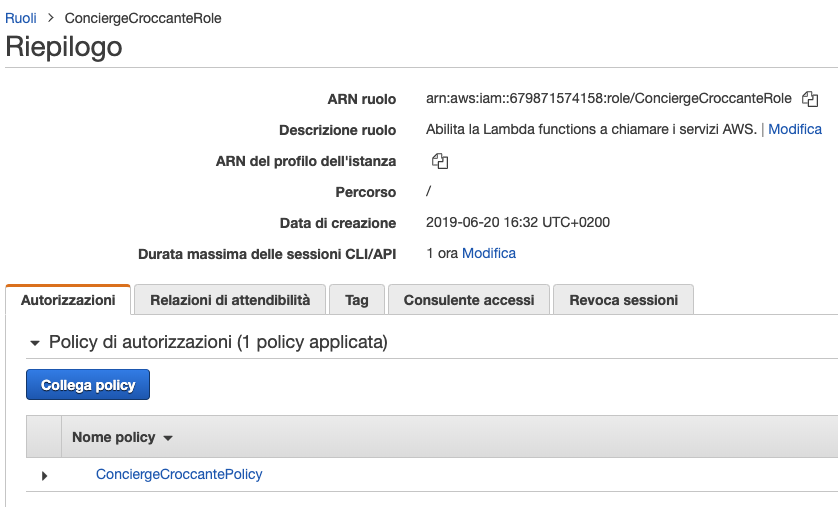
\includegraphics[width=1\columnwidth]{immagini/amazon-iam-role.png}
    \caption{\label{fig:esempio-amazon-iam-role}Esempio di Role creata}
\end{figure}

\newpage
\subsection{AWS CloudWatch}
Amazon CloudWatch\footnote{AWS CloudWatch. URL: \href{https://aws.amazon.com/it/cloudwatch/}{https://aws.amazon.com/it/cloudwatch/}} è un servizio di monitoraggio pensato per gli sviluppatori per fornire dati e analisi dal monitoraggio delle applicazioni, così da rispondere ai cambiamenti di prestazioni a livello di sistema, ottimizzare l'utilizzo delle risorse e ottenere una visualizzazione unificata dello stato di integrità operativa. CloudWatch raccoglie i dati di monitoraggio sotto forma di log, parametri ed eventi, unificando la loro visualizzazione, sulle applicazioni e i servizi eseguiti in AWS. Nel caso del progetto Concierce Croccante CloudWatch è stato utilizzato per rilevare comportamenti anomali della Skill, rilevando gli eventuali errori presenti nei log.
\begin{figure}[H] 
    \centering 
    
\includegraphics[width=0.8\columnwidth]{immagini/amazon-cloudwatch.png}
    \caption{\label{fig:icona_aws_cloudwatch}Icona AWS CloudWatch}
\end{figure}
\noindent Nel punto precedente, ovvero nel paragrafo \hyperref[aws-iam]{3.2.3}, è stato eseguito il procedimento necessario perché il servizio di CloudWatch venga abilitato. Pertanto non è necessario alcuna configurazione. Basterà recarsi al sito per poter utilizzare il servizio qualora si voglia visualizzare i dati sotto forma di log dopo o durante l'esecuzione di un servizio AWS, nel caso del progetto il servizio di AWS Lambda.

\subsection{AWS DynamoDB}
Amazon DynamoDB\footnote{AWS DynamoDB. URL: \href{https://aws.amazon.com/it/dynamodb/}{https://aws.amazon.com/it/dynamodb/}} è un servizio di database NoSQL (database non relazionale) proprietario e completamente gestito che supporta strutture di dati di tipo documento e di tipo chiave-valore. Caratteristiche di pregio sono database durevoli, multiregione e offrono sicurezza, backup, ripristino e cache in memoria per le applicazioni Internet. DynamoDB può gestire oltre 10 trilioni di richieste al giorno e supportando picchi di oltre 20 milioni di richieste al secondo. Nel progetto La Skill realizzata utilizza tale servizio per interrogare un database contenente la lista dei nomi del personale Crispy Bacon. 
\begin{figure}[H] 
    \centering 
    
\includegraphics[width=0.8\columnwidth]{immagini/amazon-dynamodb.png}
    \caption{\label{fig:icona_aws_dynamo}Icona AWS DynamoDB}
\end{figure}
\noindent È necessario quindi impostare tale servizio. Per farlo occorre recarsi nella pagina dedicata del db e una volta eseguito l'accesso con le proprie credenziali seguire le seguenti istruzioni:
\begin{itemize}
	\item Nel pannello a sinistra andare sulla sezione \texttt{Tabelle} e successivamente su \texttt{Crea Tabella};
	\item Nella nuova pagina sarà possibile settare le impostazioni della nuova tabella, quindi inserire un nome e due chiavi primarie, una di partizione e una di ordinamento, come mostra l'immagine seguente:
	\begin{figure}[H] 
        \centering 
        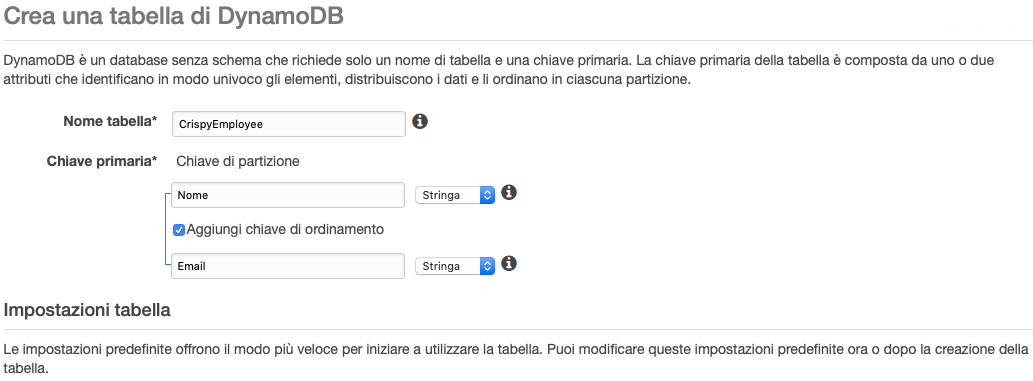
\includegraphics[width=1\columnwidth]{immagini/aws_dynamo.png}
	    \caption{\label{fig:esempio_aws_dynamo}Esempio creazione tabella AWS DynamoDB}
    \end{figure}
	
	\item Infine cliccare su \texttt{Crea}.
\end{itemize}
Ora è possibile popolare il database inserendo i dati nell'apposito pannello di controllo di DynamoDB oppure fare delle interrogazioni da codice.

\newpage
\section{Creazione della Skill}
Una volta configurati correttamente tutti i servizi di AWS che Concierge Croccante andrà ad utilizzare si è proceduti con la realizzazione vera e propria della Skill. In questa parte infatti si andrà a mostrare e spiegare come questa sia stata realizzata basandosi sull'analisi della VUI fatta al punto \hyperref[vui]{2.5}. Il processo di realizzazione della Skill parte dalla console per sviluppatori di Alexa, a seguire la creazione della funzione Lambda dove verrà eseguito il programma, terminando infine con la stesura del codice mostrando parti di esso ritenute fondamentali. 
\subsection{Alexa Developer Console}
Per creare la Skill C.C. è necessario visitare ed entrare nella console di gestione ed accedere al servizio Alexa Skills Kit\footnote{Alexa Skill Kit. URL: \href{https://developer.amazon.com/it/alexa-skills-kit}{https://developer.amazon.com/it/alexa-skills-kit}}. Una volta fatto l’accesso con le proprie credenziali si è proceduto a creare il prodotto:
\begin{itemize}
	\item Cliccare su \texttt{Create Skill} per creare la Skill;\\
	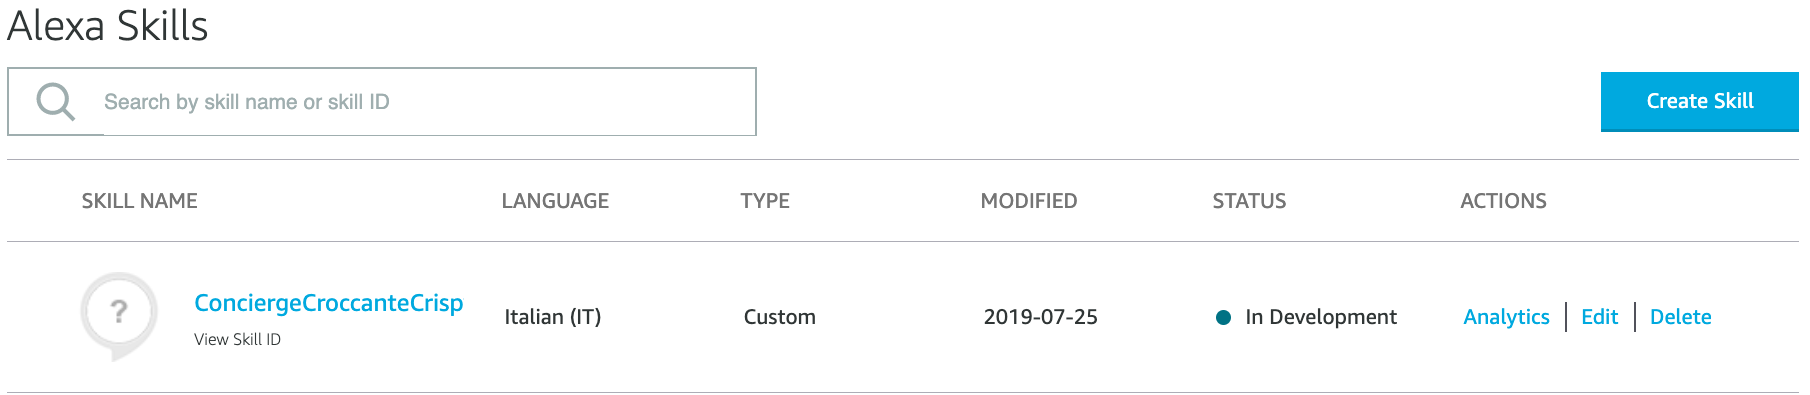
\includegraphics[width=12.5cm]{immagini/alexa-console-dev1.png}
	\item Nella pagina successiva, dare un nome alla propria Skill (facendo attenzione al fatto che quest'ultimo \textbf{non} sarà il nome di invocazione), scegliere la lingua, in questo caso \textit{Italian (IT)}, e scegliere \textit{Custom} come modello lasciando invariato il resto dei parametri. Successivamente cliccare nuovamente su \texttt{Create Skill};\\
	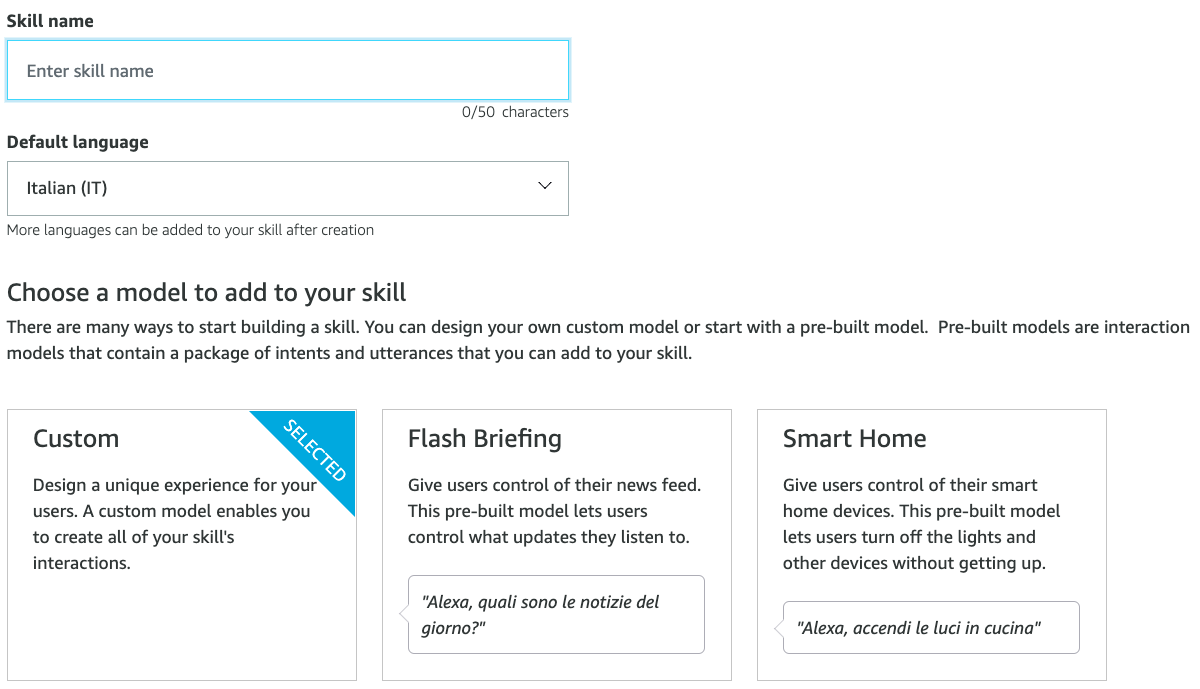
\includegraphics[width=13cm]{immagini/alexa-console-dev2.png}\\
	% 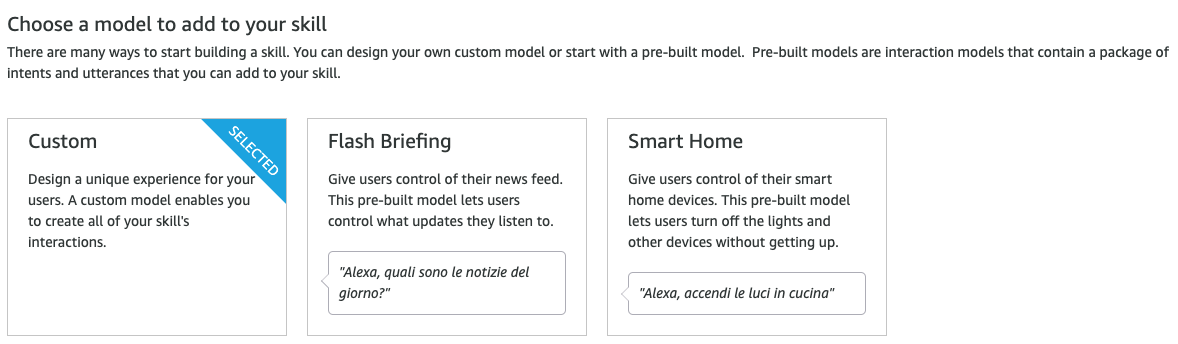
\includegraphics[width=12cm]{immagini/alexa-console-dev3.png}
	\newpage
	\item Si verrà reindirizzati nella pagina Alexa Developer Console dove sarà possibile customizzare la Skill. Nella sezione \texttt{Custom}, situata a sinistra, andare su \texttt{Invocation} per inserire il nome con cui si desidera invocare la Skill;\\[0.5cm]
	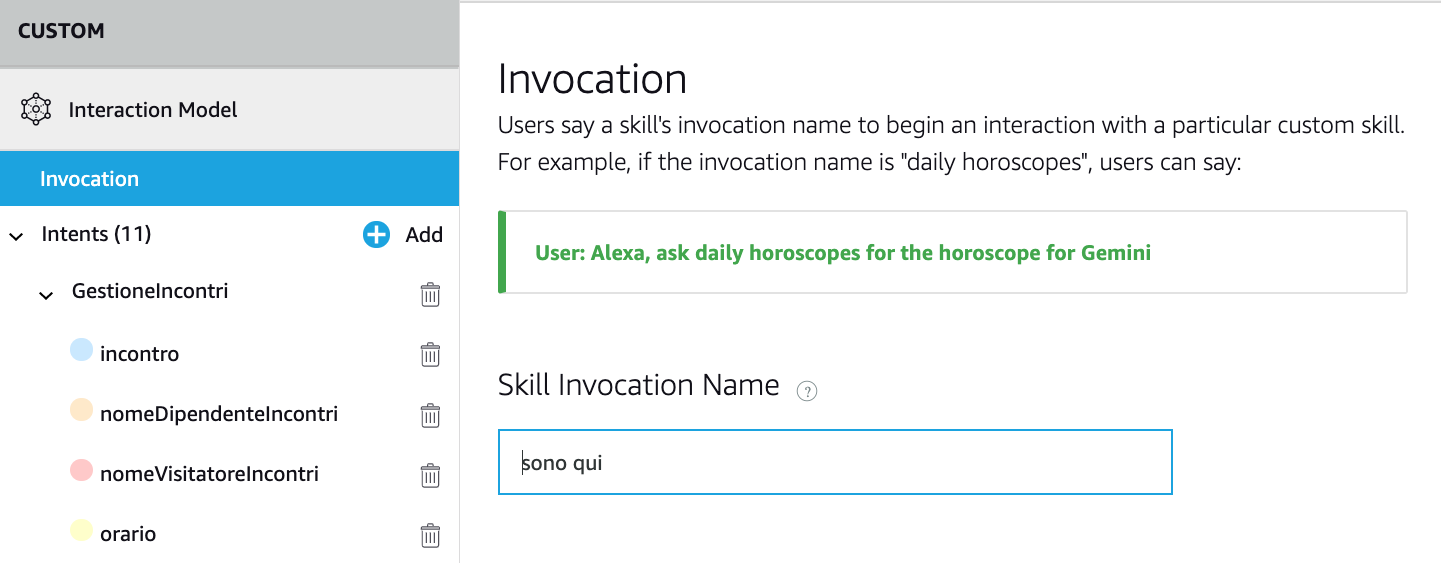
\includegraphics[width=12.5cm]{immagini/alexa-console-dev4.png}
	\item Successivamente è necessario creare gli intenti (\textit{intents}), che rappresentano un’azione che soddisfa una richiesta dell'utente. Sempre nella sezione \texttt{Custom} - \texttt{JSON Editor} è possibile creare gli intenti caricando un file .json oppure scrivendoli sull'editor della pagina. A questo punto il comando di invocazione e gli intents sono stati impostati correttamente.\\[0.5cm]
	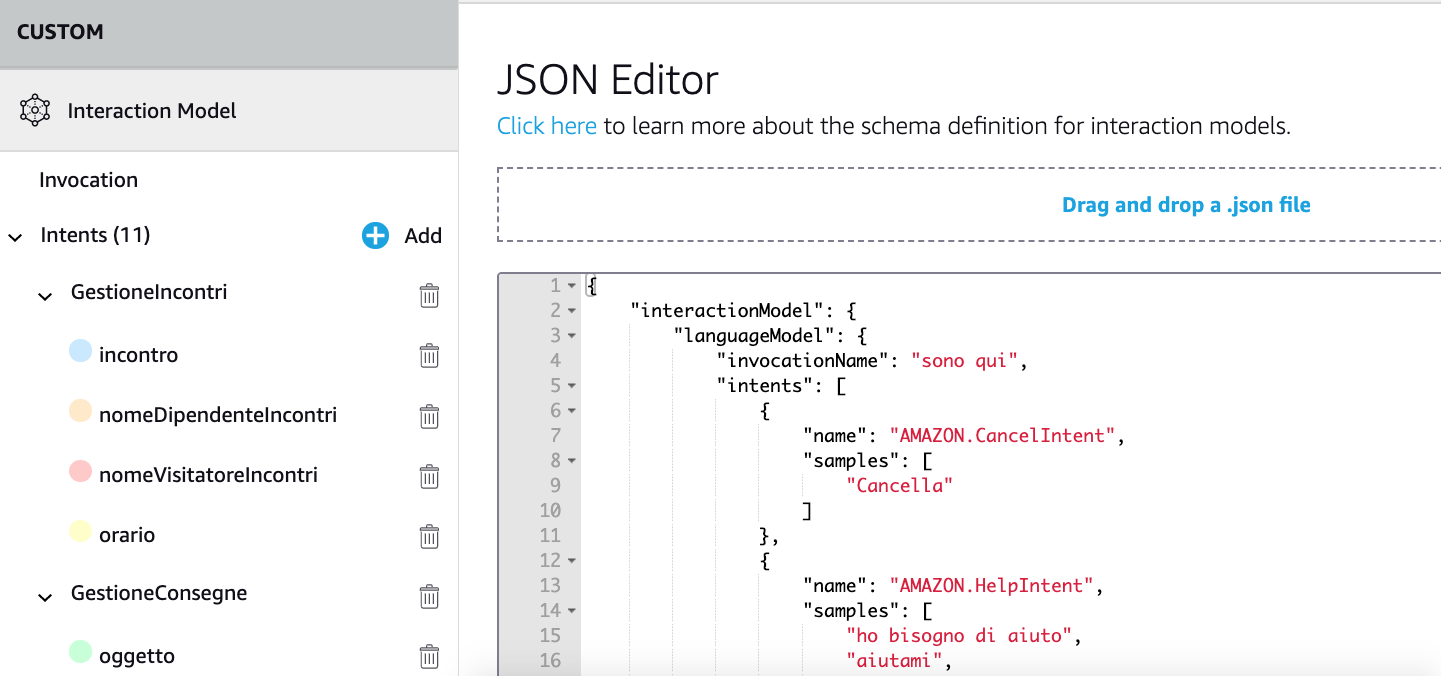
\includegraphics[width=12.5cm]{immagini/alexa-console-dev5.png}
\end{itemize}

\newpage
\noindent \subsubsection{Skill ID}
Il passo seguente è stato quello di salvare lo Skill ID, la chiave identificativa della Skill appena creata, che nei passi successi servirà per impostare l'endpoint: ovvero collegare la Skill alla Lambda dove risiederà il codice. Per fare ciò è stato sufficiente identificare e salvare l'ID inglobato nell'indirizzo URL della Skill appena creata, come mostra l'immagine seguente:
\begin{figure}[H]
	\centering
	\includegraphics[width=13cm]{immagini/url_skill.png}
	\caption{Esempio Skill ID}
\end{figure}

\subsection{AWS Lambda}
Amazon Lambda\footnote{AWS Lamba. URL: \href{https://aws.amazon.com/it/lambda/}{https://aws.amazon.com/it/lambda/}} è un servizio della suite AWS che consente di eseguire codice senza dover effettuare il provisioning\footnote{In telecomunicazioni è un servizio cloud a disposizione dell'utente che include hardware, software, cablaggio ed altro} e gestire server. Con Amazon Lambda è quindi possibile eseguire codice per qualsiasi tipo di applicazione o servizio back-end, senza alcuna amministrazione. Caricato il codice, Lambda attua tutte le azioni necessarie per eseguirlo e ricalibrare le risorse con massima disponibilità. È possibile anche configurare il codice in modo che venga attivato automaticamente da altri servizi AWS oppure che venga richiamato direttamente da qualsiasi applicazione Web o mobile.\\[0.5cm]
Una volta proceduti a creare la Skill la fase successiva è stata la realizzazione della funzione Lambda necessario per l'esecuzione del codice C.C.. Recandosi nell'omonima pagina, Amazon Lambda, sono stati eseguiti i passaggi di configurazione per creare la funzione ospitante il codice implementato o in fase di implementazione. Una volta fatto l'accesso con le proprie credenziali si è proceduto nel seguente modo:
\begin{minipage}{0.5\textwidth}
	\begin{figure}[H]
		\includegraphics[width=6cm]{immagini/aws-lambda.png}
		\caption{\label{fig:aws_lambda_regione}Selezione regione AWS Lambda}
	\end{figure}
\end{minipage}
\begin{minipage}{0.5\textwidth}
	Prima di procedere è importate cambiare la regione di esecuzione della funzione Lambda. Quindi cliccare in alto a destra sulla regione (seconda voce) e scegliere \textit{UE (Irlanda)}, come mostrato in figura. Questo passaggio è necessario perché in base alla regione scelta, AWS - Lambda mette a disposizione più o meno servizi da integrare con la funzione. Tali informazioni possono essere reperite nell'apposita pagina\footnote{Servizi per regioni. URL: \href{https://amzn.to/30GkmTd}{https://amzn.to/30GkmTd}}. Di seguito viene fornito anche URL delle \href{https://amzn.to/2NCexm7}{Regioni ed endpoint AWS}\footnote{Endpoint AWS. URL: \href{https://amzn.to/2NCexm7}{https://amzn.to/2NCexm7}} dove sono riportate le informazioni degli endpoint di ogni servizio per ciascuna regione.
\end{minipage}
\begin{itemize}
	\item Cliccare in alto a destra su \texttt{Crea funzione} per creare la Lambda;
	\item Nella pagina successiva, dare un nome alla funzione su cui verrà caricato il codice, nella sezione \texttt{runtime} scegliere \textit{Node.js 10.x} e infine nella sezione \texttt{Autorizzazioni} - \texttt{Ruolo di esecuzione} scegliere \textit{Utilizza ruolo esistente - ConciergeCroccanteRole} (ruole creato in precedenza durante la configurazione di AWS IAM al punto \hyperref[aws-iam]{3.2.3}). L'immagine seguente mostra la scelta corretta delle impostazioni base;\\[0.3cm]
	\includegraphics[width=13cm]{immagini/aws-lambda2}
	\item Successivamente cliccare nuovamente su \texttt{Crea funzione};
	\item Ora la funzione è stata impostata con le autorizzazioni sufficienti e necessarie per poter utilizzare i servizi che la Skill necessita. A destra cliccare su \texttt{Aggiungi trigger}, selezionare \texttt{Alexa Skill Kit}, inserire la Skill ID (salvata in precedenza) e cliccare su \texttt{Aggiungi}.
\end{itemize}
\subsubsection{Endpoint}
\label{endpoint}
Ora è possibile terminare il processo di configurazione della Skill eseguendo il collegamento tra Skill e Lambda. Ritornando nella console di AWS, sul servizio Lambda, è stato copiato l'indirizzo ARN della funzione, situato in alto a destra, come mostra nell'immagine seguente:
\begin{figure}[H]
	\centering
	\includegraphics[width=13cm]{immagini/aws-lambda3.png}
	\caption{Esempio URL ARN Lambda}
\end{figure}
\noindent Successivamente, nella Skill in Alexa Developer Console, nella sezione \texttt{Custom} - \texttt{Endpoint}, incollare l'URL ARN della Lambda copiato in \texttt{Default Region}.
\begin{figure}[H]
	\centering
	\includegraphics[width=13cm]{immagini/aws-lambda4.png}
	\caption{Esempio URL ARN Lambda}
\end{figure}
\noindent Infine cliccare su \texttt{Save Endpoint}. Ora la Skill l'endpoint impostato con l'esecuzione della funzione lambda creata.\\
Non rimane altro che caricare il codice del prodotto. Per farlo basterà recarsi nuovamente sulla console di AWS nel servizio Lambda, scegliere la propria funzione e su \texttt{Codice della funzione} scegliere \textit{Carica un file .zip} per caricare la cartella compressa del progetto.
\begin{figure}[H]
	\centering
	\includegraphics[width=13cm]{immagini/aws-lambda5.png}
	\caption{Codice funzione}
\end{figure}




% !TEX encoding = UTF-8
% !TEX TS-program = pdflatex
% !TEX root = ../tesi.tex

%**************************************************************
\chapter{Codifica e Validazione}
\label{cap:codifica_validazione}
Dopo aver completato la fase di progettazione è stata eseguita la fase di codifica e validazione. Questo capitolo sarà il conseguimento della seconda parte del periodo di stage dove verranno spiegate le funzionalità implementate nella Skill mostrando porzioni di codice. Verrà inoltro spiegata la struttura del progetto: le varie cartelle contenti i file delle \textit{classi} realizzate e i \textit{packages} installati. 

\section{Organizzazione del codice}
Successivamente alla parte di comprensione e configurazione dei servizi utilizzati in questo progetto, e alla creazione della Skill, è stato eseguito un micro-processo di organizzazione del codice prima della sua stesura. Questa pratica adottata è stata necessaria per avere uno schema e una gerarchia delle parti di codice che sono state sviluppate durante il periodo di tirocinio. Tale organizzazione ha permesso di sviluppare in maniera più ordinata e consapevole riducendo la probabilità di introdurre errori e rendendo il codice più manutenibile. Pertanto la cartella del progetto è stata così disposta:
\begin{itemize}
        \item \texttt{Skill}: cartella principale del progetto (main folder) contenente al suo interno altre cartelle e file organizzati secondo una determinata gerarchia
        \begin{itemize}
            \item[>] \texttt{apl-data}: cartella contenente i dati delle schermate APL;
            \item[>] \texttt{apl-template}: cartella contenente i template lo stile delle schermate APL;
            \item[>] \texttt{hendelrs}: cartella contenente i file .js di ogni handlers (gestori) creati nella Skill;
            \item[>] \texttt{i18n}: cartella contente file .js con le traduzioni della lingua;
            \item[>] \texttt{node\_modules}: cartella contenente tutti i pacchetti installati con il gestore npm;
            \item[>] \texttt{task}: cartella contente file .js da eseguire a riga di comando per l'esecuzione di funzionalità primitive;
            \item[>] \texttt{utils}: cartella contente file .js con classi di utilità, come lettura del db, invio di e-mail, ecc..;
            \item[-] \texttt{credentials.json}: file contenente delle credenziali per accedere al servizio di Google Calendar;
            \item[-] \texttt{googleAuthTokenCredential.json}: file contenente delle credenziali per accedere al servizio di Google Calendar;
            \item[-] \texttt{index.js}: file principale dove inizia l'esecuzione della Skill. La Lambda difatti partirà con la lettura di questo file;
            \item[-] \texttt{intent.json}: file .json contenente tutti gli intent creati per la Skill;
            \item[-] \texttt{package.-lock.json}: file di configurazione automaticamente creato dal gestore di pacchetti npm;
            \item[-] \texttt{package.json}: file di configurazione automaticamente creato dal gestore di pacchetti npm;
            \item[-] \texttt{policy.json}: file .json contente le regole di policy create al punto \hyperref[aws-iam]{3.2.3}.
        \end{itemize}
    \end{itemize}
\begin{figure}[H]
	\includegraphics[width=13.2cm]{immagini/skill-folder.png}
	\caption{\label{fig:gerarchia_cartella_cc}Gerarchia cartella progetto C.C.}
\end{figure}

\subsection{Handlers}
Come descritto prima la cartella del progetto C.C. è stata disposta per una gestione ordinata del codice. Una delle sotto-cartelle contenute al suo interno è dedicata per la gestione degli handlers. Nel codice della Skill gli handlers sono delle funzioni che hanno lo scopo di gestire gli eventi che vengono scatenati all'invocazione di un comando da parte dell'utente. Gli handlers sono stati così realizzati:
\begin{itemize}
    \item \texttt{index.js}: che contiene ed ingloba l'export di tutte le classi dei handlers contenuti in questa cartella;
    
    \item \texttt{gestioneConsegne\_Complete.js}: questo handler ha il compito di catturare l'evento nel caso in cui l'utente intenda consegnare un pacco (o lettera) sapendo già il nome del destinatario e, o l'oggetto consegnato o la professione dell'utente che sta conversando;
    \item \texttt{gestioneConsegne\_NomeDipendete.js}: questo handler ha il compito di catturare l'evento nel caso in cui l'utente intenda consegnare un pacco (o lettera) senza sapere già il nome del destinatario. Questo gestore ha il compito di richiedere tale dato domandandolo all'utente che sta conversando con la Skill;
    \item \texttt{gestioneIncontri\_Complete.js}: questo handler ha il compito di catturare l'evento nel caso in cui l'utente visitatore abbia un appuntamento e i dati necessari sono stati tutti raccolti;
    \item \texttt{gestioneIncontri\_NomeDipendente\_NomeVisitatore.js}: questo handelr ha il compito di catturare l'evento nel caso in cui l'utente visitatore abbia un appuntamento e, il nome del dipendetene cercato e del cliente appena entrato, sono stati raccolti. Il gestore eseguirà dei controlli per verificare l'attendibilità dei dati per poi proseguire con il dialogo oppure chiedendone di nuovi;
    \item \texttt{gestioneIncontri\_NomeDipendente.js}: questo handler ha il compito di catturare l'evento nel caso in cui l'utente abbia un appuntamento e la Skill richiede il nome del dipendente cercato;
    \item \texttt{gestioneIncontri\_Orari.js}: questo handler ha il compito di catturare l'evento nel caso in cui l'utente abbia un appuntamento e la Skill richiede l'orario per verificare l'evento nel calendario;
    \item \texttt{vorreiIncontri\_Complete.js}: questo handler ha il compito di catturare l'evento nel caso in cui l'utente visitatore desideri incontrare un dipendente e sono stati raccolti tutti i dati necessari;
    \item \texttt{vorreiIncontri\_CompleteWithOrario.js}: questo handler ha il compito di catturare l'evento nel caso in cui l'utente visitatore desideri incontrare un dipendente e richiede l'orario di appuntamento per verificare l'esistenza dell'evento nel calendario;
    \item \texttt{vorreiIncontri\_NomeDipendente\_NomeVisitatore.js}: questo handler ha il compito di catturare l'evento nel caso in cui l'utente visitatore desideri incontrare un dipendente e, il nome del dipendetene cercato e del cliente appena entrato, sono stati raccolti. Il gestore eseguirà dei controlli per verificare l'attendibilità dei dati per poi proseguire con il dialogo oppure chiedendone di nuovi;
    \item \texttt{vorreiIncontri\_NomeDipendente.js}: questo handler ha il compito di catturare l'evento nel caso in cui l'utente visitatore desideri incontrare un dipendente e la Skill richiede il nome di quest'ultimo;
    \item \texttt{vorreiIncontri\_SiNo.js}: questo handler ha il compito di catturare l'evento nel caso in cui l'utente visitatore abbia un appuntamento e la Skill ne richiede l'orario per verificare l'evento nel calendario;
    \item \texttt{touchWrapperUserEvent.js}: questo handler ha il compito di catturare gli eventi scatenati dal tocco sul display.
\end{itemize}
\begin{figure}[H]
	\includegraphics[width=13.2cm]{immagini/skill-folder2.png}
	\caption{\label{fig:gerarchia_cartella_cc2}Gerarchia cartella progetto C.C. - Handlers}
\end{figure}
\subsection{Utils}
\label{utils}
Lo stesso criterio usato per organizzare gli handlers è stato adottato anche per le classi Javascript che contengono il codice delle funzionalità della Skill. La cartella \textit{utils} contiene appunto quei metodi che permetto ad esempio la lettura del databse, l'invio di e-mail, l'invio di notifiche e la lettura del calendario. Le utilità sono state così realizzate:
\begin{itemize}
    \item \texttt{databaseUtils.js}: questa classe mette a disposizione i metodi per interrogare il database e sono presenti le seguenti funzioni:
    \begin{itemize}
        \item[>] \texttt{getInstance()}
        \item[>] \texttt{runQuery(params: var)}
        \item[>] \texttt{runScan(params: var)}
        \item[>] \texttt{runPut(params: var)}
        \item[>] \texttt{checkEmployee(nome\_dipendente: var)}
    \end{itemize}
    \item \texttt{emailUtils.js}: questa classe mette a disposizione i metodi per l'invio di messaggi e-mail ed è presente la seguente funzione:
    \begin{itemize}
        \item[>] \texttt{sendMail(from: var, to: var, message: var, oggetto: var)}
    \end{itemize}
    \item \texttt{gcalendarUtils.js}: questa classe mette a disposizione i metodi per la lettura e verifica di eventi nel calendario e sono presenti le seguenti funzioni:
    \begin{itemize}
        \item[>] \texttt{listEvents(idCalendar: var)}
        \item[>] \texttt{checkEvent(events: var, email\_dipendente: var, nome\_visitatore: var, orarioEvento: var)}
        \item[>] \texttt{generateOAuth2Client()}
    \end{itemize}
    \item \texttt{gchatUtils.js}: questa classe mette a disposizione i metodi per l'invio di notifiche su Google Chat, funzionalità in fase di sviluppo fatta nell'ultimo periodo di tirocinio, e sono presenti le seguenti funzioni:
    \begin{itemize}
        \item[>] \texttt{sendNotify(type: var, message: var)}
        \item[>] \texttt{checkThread(type: var)}
        \item[>] \texttt{putThread(thread: var, thread\_type: var)}
    \end{itemize}
    \item \texttt{prepareQuery.js}: questa classe mette a disposizioni i metodi per ricevere le query di interrogazione che si desidera e sono presenti le seguenti funzioni:
    \begin{itemize}
        \item[>] \texttt{scanEmployee()}
        \item[>] \texttt{queryEmployee(nomeDipendente: var)}
        \item[>] \texttt{putThread()}
        \item[>] \texttt{updateThread(old\_thread: var, new\_thread: var)}
    \end{itemize}
    \item \texttt{slacknotifyUtils.js}: questa classe mette a disposizione i metodi per l'invio di notifiche su Slack e al suo interno sono presenti le seguenti funzioni:
    \begin{itemize}
        \item[>] \texttt{sendNotify(channel: var, message: var)}
        \item[>] \texttt{sendDirectlyNotify(member: var, MESSAGE: var)}
        \item[>] \texttt{addTag(toTag: var)}
        \item[>] \texttt{listMembersApl(intent: var)}
        \item[>] \texttt{getIdMember(toTag: var)}
        \item[>] \texttt{membersList()}
    \end{itemize}
    \item \texttt{abracadabraUtils.js}: questo metodo contiene un easter egg\footnote{Un easter egg in informatica è un contenuto di natura bizzarra e innocuo che gli sviluppatori nascondono all'interno del prodotto}
\end{itemize}
\begin{figure}[H]
	\includegraphics[width=13cm]{immagini/skill-folder3.png}
	\caption{\label{fig:gerarchia_cartella_cc3}Gerarchia cartella progetto C.C. - Utils}
\end{figure}

\section{Package utilizzati}
Particolare attenzione va fatta sulla gestione dei pacchetti e quali di essi sono stati installati nel progetto Concierge Croccante. Per tale necessità è stato utilizzato il gestore di pacchetti npm, menzionato in precedente al punto \hyperref[npm]{1.5.4}, che ha consentito di installare in maniera sicura e immediata i pacchetti necessari. Installando tali pacchetti il gestore ha suddiviso il codice all'interno di una directory chiamata \texttt{node\_modules} creando inoltre un file di configurazione delle installazioni fatte.
\begin{figure}[H]
	\includegraphics[width=12cm]{immagini/logo-npm.png}
	\caption{\label{fig:logo_npm}Logo NPM}
\end{figure}
\noindent In questa fase di progetto si è provveduto ad installare npm e tutti i pacchetti necessari alla Skill Concierge Croccante nel seguente modo:
\begin{itemize}
    \item Dalla documentazione di npm\footnote{Doc npm. URL: \href{https://docs.npmjs.com/downloading-and-installing-node-js-and-npm}{https://docs.npmjs.com/downloading-and-installing-node-js-and-npm}} viene riportato il seguente comando da eseguire su terminale:
    \begin{lstlisting}[language=bash]
		$ [sudo] npm install npm -g
	\end{lstlisting}
	Il comando installerà l'ultima versione del gestore pacchetti. Se si desidera verificare e visualizzare l'ultima versione di npm è necessario eseguire il comando: 
	\begin{lstlisting}[language=bash]
		$ npm -v
	\end{lstlisting}
	\item I pacchetti installati nel progetto sono stati i seguenti:
	\begin{itemize}
	    \item[>] \texttt{ask-sdk} e \texttt{ask-sdk-core} di AWS che semplifica la creazione di Skill, permettendo di utilizzare le funzionalità base di Alexa in maniera rapida:
	    \begin{lstlisting}[language=bash]
		    $ npm install --save ask-sdk
		    $ npm install --save ask-sdk-core
	    \end{lstlisting}
	    \item[>] \texttt{request} per semplificare ed effettuare chiamate http, supporta HTTPS i re-indirizzamenti:
	    \begin{lstlisting}[language=bash]
		    $ npm install request
	    \end{lstlisting}
	    \item[>] \texttt{googleapis} è una libreria client per l'utilizzo delle API di Google, rendendo più semplice ed immediate le chiamate ai servizi come Calendar:
	    \begin{lstlisting}[language=bash]
		    $ npm install googleapis
	    \end{lstlisting}
	    \item[>] \texttt{slack-notify} è una libreria che rende flessibile l'utilizzo dell'API Webhooks\footnote{Incoming Webhooks. URL: \href{https://api.slack.com/incoming-webhooks}{https://api.slack.com/incoming-webhooks}} di Slack, semplificando l'invio di notifiche a Slack dalla Skill:
	    \begin{lstlisting}[language=bash]
		    $ npm install slack-notify
	    \end{lstlisting}
	    \item[>] \texttt{i18next} e \texttt{i18next-sprintf-postprocessor} sono dei framework di internazionalizzazione popolari ambienti javascript:
	    \begin{lstlisting}[language=bash]
		    $ npm install i18next
		    $ npm install i18next-sprintf-postprocessor
	    \end{lstlisting}
	\end{itemize}
\end{itemize}

\newpage
\section{Calendario}
Per la soddisfazione del requisito RO17 analizzato al punto \hyperref[requisti-richiesti]{2.3}, ovvero la lettura e verifica degli appuntamenti in calendario, è stato richiesto l'uso di Google Calendar, già utilizzato dall'azienda Crispy Bacon per le sue note funzionalità. 
\subsection{Google Calendar}
Per l’integrazione col servizio di Google Calendar sono a disposizione delle API documentate reperibili al indirizzo \href{https://developers.google.com/calendar/}{developers.google.com/calendar/}. Dalla guida emergono i seguenti requisti necessari:\\
\begin{minipage}{0.5\textwidth}
	\begin{figure}[H]
		\includegraphics[width=5cm]{immagini/google_calendar.png}
		\caption{\label{fig:icona_google_calendar}Icona Google Calendar}
	\end{figure}
\end{minipage}
\begin{minipage}{0.5\textwidth}
	\begin{itemize}
		\item Node.js
    	\item googleapis package
    	\item Account Google funzionante e verificato
    	\item Autorizzazione OAuth\footnote{OAuth: protocollo di rete open e standard, progettato per lavorare con il protocollo HTTP.}
	\end{itemize}
\end{minipage}
\\[0.5cm]
Nei punti successivi verranno analizzati aspetti importanti, con esempi di codice, riguardante l'integrazione con il calendario in questione e l’uso delle sue API.
\subsubsection{OAuth2}
Per consentire la lettura ed ottenere la lista di eventi presenti nel calendario è stato necessario eseguire un'autenticazione tramite il protocollo OAuth 2.0\footnote{OAuth 2.0. URL: \href{https://oauth.net/2/}{https://oauth.net/2/}}. Quest'ultimo è un protocollo di rete open che consente l'emissione di un token di accesso da parte di un server autorizzato ad un client di terze parti, nel nostro caso il servizio di Google Calendar, previa approvazione dell'utente proprietario della risorsa cui si intende accedere. Per poter ottenere ciò sono stati svolti i seguenti passi:
\begin{itemize}
    \item Visitando la pagina Google Calendar API\footnote{G. Calendar API. URL: \href{https://developers.google.com/calendar/quickstart/nodejs}{https://developers.google.com/calendar/quickstart/nodejs}} è stato abilitato l'utilizzo delle API per il calendario. Nella pagina infatti è presente il primo step da seguire dal titolo ”\textit{Turn on the Google Calendar API}” dove presente il bottone adibito all'abilitazione:\\
    \includegraphics[width=12cm]{immagini/google_calendar_api.png}\\[2cm]
    Nella sezione corrente, una volta cliccato il tasto \texttt{ENABLE THE GOOGLE CALENDAR API} ed eseguito l’accesso con l’account Google il quale si desidera leggere gli eventi in calendario, è stato salvato il file credentials.json ottenuto dall'accesso e fornito nella cartella di progetto.
    \item Sempre nella stessa pagina è stato copiato ed eseguito l'esempio di set up riportato per ottenere l’OAuth necessario a visualizzare gli eventi nel calendario. Di seguito si riporta tale esempio di codice, importante appunto per ricevere le autorizzazioni necessarie:\\[0.1cm]
	\lstinputlisting[caption=Esempio Set up Google Calendar]{code/generateGoogleAuthToken.js}
	\item Per eseguire tale esempio di codice è stato sufficiente aprire il terminale sulla cartella di progetto dove risiede il file di set up e lanciare lo script con il seguente comando:
	\begin{lstlisting}[language=bash]
		$ node [filename]
	\end{lstlisting}
	Nel caso in cui fosse la prima volta che viene eseguito tale esempio è necessario autorizzare l'accesso:
	\begin{enumerate}
		\item Aprire l'URL restituito dal terminale col proprio web browser
		\item Fare il login se non si è già loggati
		\item Cliccare il tasto \texttt{Accept}
		\item Copiare il codice ricevuto, incollarlo nella terminale e premere \texttt{Enter}
	\end{enumerate}
\end{itemize}
\subsubsection{Lettura eventi}
All'interno del progetto Concierge Croccante la fase di lettura del calendario è stata semplificata realizzando una classe contenente al suo interno metodi appositi. Di tali metodi, già menzionati al punto \hyperref[utils]{3.4.2}, ne viene riportato il codice e analizzato il loro funzionamento:
\lstinputlisting[caption=Metodi listEvent e generateOAuth2Client]{code/gcalendarUtils1.js}
Per ottenere la lista di eventi non servirà altro che richiamare \texttt{listEvents(idCalendar)}. La funzione ritornerà un oggetto contenente tutti gli eventi, con le loro informazioni, della giornata odierna fino ad un massimo di 15 risultati. Attenzione: i file citati credentials.json e googleAuthTokenCredential.json non sono altro che le credenziali recuperate nei punti precedenti per accedere con il token OAuth.
\\[0.5cm]
Altro metodo presente e largamente utilizzato è \texttt{checkEvent(events, email\_dipendente, nome\_visitatore, orarioEvento)}:
\\[0.1cm]
\lstinputlisting[caption=Metodo checkEvent]{code/gcalendarUtils2.js}
Questo metodo pone come precondizione il fatto di ricevere in ingresso l'elenco di eventi ed i seguinti valori: nome visitatore, nome persona cercata ed orario; non vuoti. Il risultato sarà un valore \textit{boolean false} nel caso \textbf{non} sia presente alcun evento nel calendario, un valore numerico \textit{1} nel caso sia stato trovato un evento per la persona e l'orario indicato, oppure \textit{0} se esiste un evento ma l'orario indicato non coincide con quello effettivo.

\newpage
\section{Invio notifiche}
Altra specifica per la soddisfazione dei requisiti RO18 e RO19 analizzati al punto \hyperref[requisti-richiesti]{2.3}, è l'invio di notifiche. Per ovviare a ciò sono state realizzate le funzionalità per l'invio di messaggi istantanei via Slack e e-mail via AWS SES visto il già utilizzo di questi servizi da parte di Crispy Bacon.
\subsection{Slack}
Per l’integrazione col servizio di Slack sono a disposizione delle API documentate reperibili al indirizzo \href{https://api.slack.com/}{api.slack.com/}. Dalla guida emergono i seguenti requisti necessari:
\\
\begin{minipage}{0.5\textwidth}
	\begin{figure}[H]
		\includegraphics[width=6cm]{immagini/slack.png}
		\caption{\label{fig:icona_slack}Icona servizio - Slack}
	\end{figure}
\end{minipage}
\begin{minipage}{0.5\textwidth}
	\begin{itemize}
		\item Node.js
		\item slack-notify package
		\item Account Slack
		\item Incoming Webhook
	\end{itemize}
\end{minipage}
\\[0.4cm]
Nei punti successivi verranno analizzati aspetti importanti, con esempi di codice, riguardante l'invio di notifiche con Slack e l’uso delle sue API.
\subsubsection{Incoming Webhooks}
Per consentire l'invio di messaggi di notifica via chat viene scelto di utilizzare un bot con Incoming Webhook\footnote{Incoming Webhooks. URL: \href{https://api.slack.com/incoming-webhooks}{https://api.slack.com/incoming-webhooks}}. Quest'ultimo è un mezzo con il quale si semplifica l'invio di messaggi da un'applicazione a Slack. La creazione di un Incoming Webhook fornisce un URL univoco a cui si invia un payload JSON con il testo del messaggio e alcune opzioni.
Per ottenere l'Incoming Webhook sono stati eseguiti i seguenti passaggi:
\begin{itemize}
    \item Visitando la pagina dedicata \href{https://api.slack.com/incoming-webhooks}{api.slack.com/incoming-webhooks} è stata creata un'App per Slack cliccando sul tasto \texttt{"Create your Slack app"}:\\
    \includegraphics[width=12cm]{immagini/slack_bot.png}\\
    Si viene successivamente indirizzati in una nuova pagina dove sarà possibile creare la propria App per Slack:
	\begin{enumerate}
		\item Cliccare sul tasto \texttt{Create New App}
		\item Inserire il nome dell'app
		\item Scegliere lo \textit{space} di lavoro dove installare l'app
		\item Cliccare su \texttt{Crea App}
	\end{enumerate}
	\item Dopo aver creato l'App è stato abilitato l'Incoming Webhook nell'apposita pagina delle impostazioni. Dopo aver fatto ciò sono state visualizzate alcune opzioni aggiuntive. Tra queste era presente il pulsante \textit{Aggiungi nuovo Webhook a Workspace}. Viene quindi aggiunto il Webhook ad canale/space di Slack designato per pubblicare l'App e salvata tale modifica facendo clic su \texttt{Autorizza la tua app}.
\end{itemize} 
\subsubsection{Invio messaggi}
All'interno del progetto Concierge Croccante la fase di notifica via Slack è stata semplificata realizzando una classe contenente al suo interno metodi appositi. Di tali metodi menzionati al punto \hyperref[utils]{3.4.2} ne viene riportato il codice e analizzato il loro funzionamento\footnote{NB: la variabile \texttt{MY SLACK WEBHOOK URL} contiene l'URL del Webhook dell'App}: 
\\[0.1cm]
\lstinputlisting[caption=Metodo sendNotify]{code/slacknotifyUtils1.js}
Il codice sopra riportato mostra il metodo \texttt{sendNotify(channel:  var, message:  var)}: tale funzione non fa altro che inviare il testo del messaggio nel canale di Slack desiderato passando i dati per parametro. La variabile constante \texttt{slack.send} richiama il metodo fornito del pacchetto \texttt{slack-notify} che non farà altro che fare una \textit{request} in \textit{POST} all'API \texttt{chat.postMessage}. Nel caso in cui il metodo riscontrasse un errore nell'invio del messaggio viene lanciata un eccezione.

\newpage
\lstinputlisting[caption=Metodo sendDirectlyNotify]{code/slacknotifyUtils2.js}
Per l'invio delle notifiche in direct message\footnote{Messaggio privato inviato in un social media} è stato messo a disposizione il metodo \texttt{sendDirectlyNotify(member:  var, MESSAGE:  var)}: tale funzione invierà il testo del messaggio al destinatario indicato alla funzione facendo, anche in questo caso, una \textit{request} in \textit{POST} all'API \texttt{chat.postMessage}. Differentemente dal metodo precedente qui non viene utilizzata alcuna libreria, ma viene usata l'API in maniera diretta.

\newpage
\lstinputlisting[caption=Metodo addTag]{code/slacknotifyUtils3.js}
Altra funzionalità messa a disposizione dalla classe è il metodo \texttt{addTag(toTag: var)}: tale funzione non fa altro che richiamare una funzione ausiliaria e privata della classe, più elaborata e non visibile all'utente esterno, che va ad aggiungere, grazie all'id del membro cercato, il tag necessario per menzionarlo all'interno delle chat di gruppo.

\newpage
\lstinputlisting[caption=Metodo listMembersApl]{code/slacknotifyUtils4.js}
Metodo più rilevante è \texttt{listMembersApl(intent: var)}: tale metodo viene richiamato dalla Skill qualora fosse necessaria la costruzione di un APL con elementi touch che al momento del tocco scatenino un evento. In questo caso l'APL che si va a creare è una lista dei membri di Crispy Bacon dove è possibile selezionare il nome per fornirlo alla Skill. 

\newpage
\subsection{E-mail}
Per l'invio di notifiche via e-mail, come già detto in precedenza, è stato utilizzato il servizio Amazon SES e la sua integrazione con il servizio sono necessari i seguenti requisiti:
\\
\begin{minipage}{0.47\textwidth}
	\begin{figure}[H]
		\includegraphics[width=6cm]{immagini/ses.png}
		\caption{\label{fig:google_calendar}Icona servizio - SES}
	\end{figure}
\end{minipage}
\begin{minipage}{0.5\textwidth}
	\begin{itemize}
		\item Node.js
		\item npm aws-sdk
		\item Account AWS
		\item Indirizzo e-mail
	\end{itemize}
\end{minipage}
\\[0.4cm]
Nei punti successivi verranno analizzati aspetti importanti, con esempi di codice, riguardante l'invio di e-mail con Amazon SES e l'uso della libreria SDK.

\subsubsection{Invio e-mail}
All'interno del progetto Concierge Croccante l'invio di notifiche o messaggi via e-mail è stata semplificata realizzando una classe contenente al suo interno metodi appositi. Di tali metodi menzionati al punto \hyperref[utils]{3.4.2} ne viene riportato il codice e analizzato il loro funzionamento: 
\\[0.1cm]
\lstinputlisting[caption=Metodo sendMail]{code/emailUtils.js}
Il codice sopra riportato mostra il metodo \texttt{sendMail(from:  var, to:  var, message:  var, oggetto:  var)}: tale funzione non fa altro che inviare una e-mail con i campi from, to, message ed oggeto passati per parametro. La variabile constante \texttt{ses} non fa altro che richiamare il metodo fornito del pacchetto \texttt{aws-sdk} che si occuperà di richiamare le API necessarie all'utilizzo di AWS SES.

\newpage
\section{Lettura del Database}
Funzionalità a supporto di quelle principali è la lettura del database DynamoDB. Quest'ultimo è popolato da una tabella contente i nomi di tutti i dipendenti dell'azienda Crispy Bacon, i quali, vengono prelevati per essere utilizzati nelle fasi di controllo, come la ricerca di un dipendente per verificarne la sua esistenza. Il progetto predispone due classi adibite a questo tipo di funzionalità per interrogare il database: \texttt{databaseUtils.js} e \texttt{prepareQuery.js}.
\\[0.1cm]
\lstinputlisting[caption=Metodo getInstance e runQuery]{code/databaseUtils.js}
Il codice sopra riportato mostra la classe coi metodi per eseguire \textit{query} di diversa tipologia: \texttt{runQuery(params:  var)} non fa altro che richiamare il metodo presente nel pacchetto \texttt{aws-sdk} per l'esecuzione di un interrogazione standard. Altri metodi come \texttt{runScan(params:  var)} e \texttt{runPut(params:  var)} eseguono una scansione e un inserimento nel database secondo i parametri\footnote{La classe \texttt{prepareQuery.js} svolge perll'appunto questo ruolo. I metodi della classe ritornano un oggetto contente i parametri necessari per l'esecuzione della query desiderata} passati alle funzioni.

\newpage
\section{Async e Await}
Nella fase di stesura del codice durante il periodo di tirocinio è stato affrontato e studiato il tema della chiamate asincrone: Async/await functions. Questo modello di funzioni va inserito nel contesto delle \textit{Promise} che, come suggerisce il suo nome, restituisce un risultato nel futuro che può essere di tipo \textit{resolve}, nel caso di successo nell'azione svolta, o \textit{reject} nel caso di un fallimento con conseguenza di errore. Per fare ciò la sintassi async/await permette di lavorare con le \textit{Promise} in un modo più confortevole e facile da usare. Per spiegare il significato di questa sintassi vengono fatti i seguenti esempi estratti dal codice della Skill Concierge Croccante. Il seguente esempio mostra una funzione che ritorna una promessa, ovvero un risultato dopo aver eseguito determinati calcoli. In questo caso ritorna una Promise con \textit{resolve} nel caso di un risultato da parte della chiamata API:
\\[0.1cm]
\lstinputlisting[caption=Esempio codice con Promise]{code/promise.js}
\noindent È necessario ora che la funzione chiamante il metodo \texttt{getIdMember(toTag: var)} attenda il risultato della \textit{Promise} prima di proseguire con le istruzioni successive. Il modello async/await risolve tale necessità: dichiarando la funzione principale async e mettendo la keyword await davanti alla chiamata del metodo \texttt{getIdMember(toTag: var)} si attenderà il risultato ritornato da quest'ultima.
\\[0.1cm]
\lstinputlisting[caption=Esempio codice con Promise]{code/async_await.js}

\newpage
\section{Verifica e Validazione}
\label{cap:verifica_validazione}
%**************************************************************
L'ultima fase del periodo di tirocinio ha riguardato il processo di verifica e validazione. La prima è un processo che si occupa di fornire evidenza oggettiva, ovvero che i risultati ottenuti come output dello sviluppo del software soddisfino i requisiti, la seconda invece è un processo per confermare in modo definitivo che le caratteristiche del software siano conformi ai bisogni dell'utente e all'uso previsto.
Per eseguire la verifica e la validazione è necessario l'esecuzione di test\footnote{In ambito informatico i test eseguiti nel processo di verifica sono eseguiti in maniera automatica durante lo sviluppo del software} che individuino carenze, correttezza e affidabilità. Nel progetto della Skill Concierge Croccante non è stato realizzato alcun test per il processo di verifica: viste le tempistiche non è stato potuto fare ciò e si è pertanto scelto di eseguire test già esistenti nel servizio Amazon Lambda, sufficienti ad esaminare il codice e rilevare eventuali errori. Per quanto riguarda il processo di validazione\footnote{Attività di supporto la quale accerta che il prodotto dei processi rispetti le specifiche} è stato svolto, alla fine del periodo di tirocinio, un incontro  con il tutor aziendale e CFO Damiano Buscemi come conferma fiale la quale ha accertato le bontà richieste dal prodotto finale. Tale validazione non è stata altro che una dimostrazione funzionante della Skill, eseguita prima da me per spiegare le varie funzionalità, ed infine da Crispy Bacon come conferma.
\\[0.5cm]
\noindent Per quanto riguarda l'integrazione coi servizi utilizzati, nello specifico Google Calendar e Slack, sono stati creati dei file appositi da eseguire manualmente che verificano il corretto funzionamento di essi restituendo un risultato:
\\[0.1cm]
\begin{figure}[H]
	\includegraphics[width=13.2cm]{immagini/test-googleCalendar.png}
	\caption{\label{fig:test_googleCalendar}Esempio test funzionamento Google Calendar - Lista eventi}
\end{figure}
\newpage
\noindent L'immagine mostra l'esecuzione del file getListEventGoogleCallendar-WithOAuth.js adibito a verificare la validità del token OAuth per ottenere la lista di eventi della giornata corrente. Inoltre verifica la corretta chiamata dell'API \texttt{calendar.events.list}.
\\[0.1cm]
\begin{figure}[H]
	\includegraphics[width=13.2cm]{immagini/test-sendSlack.png}
	\caption{\label{fig:test_slack_send}Esempio test funzionamento Slack - Invio messaggio}
\end{figure}
\noindent L'immagine mostra l'esecuzione del file sendSlackMessage.js adibito a verificare la validità del token per inviare messaggi di notifica via Slack. Inoltre verifica la corretta chiamata dell'API \texttt{chat.postMessage}.
\\[0.1cm]
\begin{figure}[H]
	\includegraphics[width=13.2cm]{immagini/test-listSlack.png}
	\caption{\label{fig:test_slack_list}Esempio test funzionamento Slack - Lista membri}
\end{figure}
\noindent L'immagine mostra l'esecuzione del file getSlackListMemebers.js adibito a verificare la validità del token per ottenere la lista dei membri di Crispy Bacon. Inoltre verifica la corretta chiamata dell'API \texttt{users.list}.


   
%% !TEX encoding = UTF-8
% !TEX TS-program = pdflatex
% !TEX root = ../tesi.tex

%**************************************************************
\chapter{Analisi dei requisiti}
\label{cap:analisi-requisiti}
%**************************************************************

\intro{Breve introduzione al capitolo}\\

\section{Casi d'uso}

Per lo studio dei casi di utilizzo del prodotto sono stati creati dei diagrammi.
I diagrammi dei casi d'uso (in inglese \emph{Use Case Diagram}) sono diagrammi di tipo \gls{uml} dedicati alla descrizione delle funzioni o servizi offerti da un sistema, così come sono percepiti e utilizzati dagli attori che interagiscono col sistema stesso.
Essendo il progetto finalizzato alla creazione di un tool per l'automazione di un processo, le interazioni da parte dell'utilizzatore devono essere ovviamente ridotte allo stretto necessario. Per questo motivo i diagrammi d'uso risultano semplici e in numero ridotto.

\begin{figure}[!h] 
    \centering 
    \includegraphics[width=0.9\columnwidth]{usecase/scenario-principale} 
    \caption{Use Case - UC0: Scenario principale}
\end{figure}

\begin{usecase}{0}{Scenario principale}
\usecaseactors{Sviluppatore applicativi}
\usecasepre{Lo sviluppatore è entrato nel plug-in di simulazione all'interno dell'IDE}
\usecasedesc{La finestra di simulazione mette a disposizione i comandi per configurare, registrare o eseguire un test}
\usecasepost{Il sistema è pronto per permettere una nuova interazione}
\label{uc:scenario-principale}
\end{usecase}

\section{Tracciamento dei requisiti}

Da un'attenta analisi dei requisiti e degli use case effettuata sul progetto è stata stilata la tabella che traccia i requisiti in rapporto agli use case.\\
Sono stati individuati diversi tipi di requisiti e si è quindi fatto utilizzo di un codice identificativo per distinguerli.\\
Il codice dei requisiti è così strutturato R(F/Q/V)(N/D/O) dove:
\begin{enumerate}
	\item[R =] requisito
    \item[F =] funzionale
    \item[Q =] qualitativo
    \item[V =] di vincolo
    \item[N =] obbligatorio (necessario)
    \item[D =] desiderabile
    \item[Z =] opzionale
\end{enumerate}
Nelle tabelle \ref{tab:requisiti-funzionali}, \ref{tab:requisiti-qualitativi} e \ref{tab:requisiti-vincolo} sono riassunti i requisiti e il loro tracciamento con gli use case delineati in fase di analisi.

\newpage

\begin{table}%
\caption{Tabella del tracciamento dei requisti funzionali}
\label{tab:requisiti-funzionali}
\begin{tabularx}{\textwidth}{lXl}
\hline\hline
\textbf{Requisito} & \textbf{Descrizione} & \textbf{Use Case}\\
\hline
RFN-1     & L'interfaccia permette di configurare il tipo di sonde del test & UC1 \\
\hline
\end{tabularx}
\end{table}%

\begin{table}%
\caption{Tabella del tracciamento dei requisiti qualitativi}
\label{tab:requisiti-qualitativi}
\begin{tabularx}{\textwidth}{lXl}
\hline\hline
\textbf{Requisito} & \textbf{Descrizione} & \textbf{Use Case}\\
\hline
RQD-1    & Le prestazioni del simulatore hardware deve garantire la giusta esecuzione dei test e non la generazione di falsi negativi & - \\
\hline
\end{tabularx}
\end{table}%

\begin{table}%
\caption{Tabella del tracciamento dei requisiti di vincolo}
\label{tab:requisiti-vincolo}
\begin{tabularx}{\textwidth}{lXl}
\hline\hline
\textbf{Requisito} & \textbf{Descrizione} & \textbf{Use Case}\\
\hline
RVO-1    & La libreria per l'esecuzione dei test automatici deve essere riutilizzabile & - \\
\hline
\end{tabularx}
\end{table}%             
%% !TEX encoding = UTF-8
% !TEX TS-program = pdflatex
% !TEX root = ../tesi.tex

%**************************************************************
\chapter{Progettazione e codifica}
\label{cap:progettazione-codifica}
%**************************************************************

\intro{Breve introduzione al capitolo}\\

%**************************************************************
\section{Tecnologie e strumenti}
\label{sec:tecnologie-strumenti}

Di seguito viene data una panoramica delle tecnologie e strumenti utilizzati.

\subsection*{Tecnologia 1}
Descrizione Tecnologia 1.

\subsection*{Tecnologia 2}
Descrizione Tecnologia 2

%**************************************************************
\section{Ciclo di vita del software}
\label{sec:ciclo-vita-software}

%**************************************************************
\section{Progettazione}
\label{sec:progettazione}

\subsubsection{Namespace 1} %**************************
Descrizione namespace 1.

\begin{namespacedesc}
    \classdesc{Classe 1}{Descrizione classe 1}
    \classdesc{Classe 2}{Descrizione classe 2}
\end{namespacedesc}


%**************************************************************
\section{Design Pattern utilizzati}

%**************************************************************
\section{Codifica}
             
% !TEX encoding = UTF-8
% !TEX TS-program = pdflatex
% !TEX root = ../tesi.tex

%**************************************************************
\chapter{Verifica e validazione}
\label{cap:verifica-validazione}
%**************************************************************             % Product Design Freeze e SOP
% % !TEX encoding = UTF-8
% !TEX TS-program = pdflatex
% !TEX root = ../tesi.tex

%**************************************************************
\chapter{Conclusioni}
\label{cap:conclusioni}
%**************************************************************

%**************************************************************
\section{Consuntivo finale}

%**************************************************************
\section{Raggiungimento degli obiettivi}

%**************************************************************
\section{Conoscenze acquisite}

%**************************************************************
\section{Valutazione personale}
             % Conclusioni
\appendix                               
% !TEX encoding = UTF-8
% !TEX TS-program = pdflatex
% !TEX root = ../tesi.tex

%**************************************************************
\chapter{Appendice A}
%**************************************************************

\epigraph{Citazione}{Autore della citazione}



             % Appendice A

%**************************************************************
% Materiale finale
%**************************************************************
\backmatter
% \printglossaries
% !TEX encoding = UTF-8
% !TEX TS-program = pdflatex
% !TEX root = ../tesi.tex

%**************************************************************
% Bibliografia
%**************************************************************

\cleardoublepage
\chapter{Bibliografia}

\nocite{*}
% Stampa i riferimenti bibliografici
\printbibliography[heading=subbibliography,title={Riferimenti bibliografici},type=book]

% Stampa i siti web consultati
\printbibliography[heading=subbibliography,title={Siti web consultati},type=online]


\end{document}
